% !TeX spellcheck = en_US
% !TeX encoding = UTF-8
\documentclass[a4paper]{article}
\usepackage{graphics, graphicx}
\usepackage{fancyvrb, enumerate}
\usepackage{amsmath, amssymb, amscd, amsfonts}
\usepackage{geometry}
\usepackage{multirow}
\usepackage{url}
\usepackage{listings, listing}
\usepackage{color}
\usepackage{mathptmx}
\usepackage[numberedbib]{apacite}
\usepackage[style=iso]{datetime2}
\usepackage{csvsimple, booktabs}
\usepackage[maxfloats=256]{morefloats}
\maxdeadcycles=1000

\geometry
{
    top = 20mm,
    bottom = 20mm,
    left = 20mm,
    right = 20mm
}

\title{Periodontitis}
\author{
    Jaewoong Lee
    \and
    Seunghoon Kim
    \and
    Semin Lee
}
\date{\today}

\begin{document}
   	\maketitle
    \newpage

    \tableofcontents
    \listoftables
    \listoffigures
    \newpage

    \section{Introduction}
        \subsection{Microbiome}
            Microbiome is consist of microbiota, the micro-organisms which live inside and on humans \cite{microbiome1}. Microbiome is also about $10^{13}$ micro-organisms whose which collective genome \cite{microbiome2}.

            \begin{figure}[p]
                \centering
                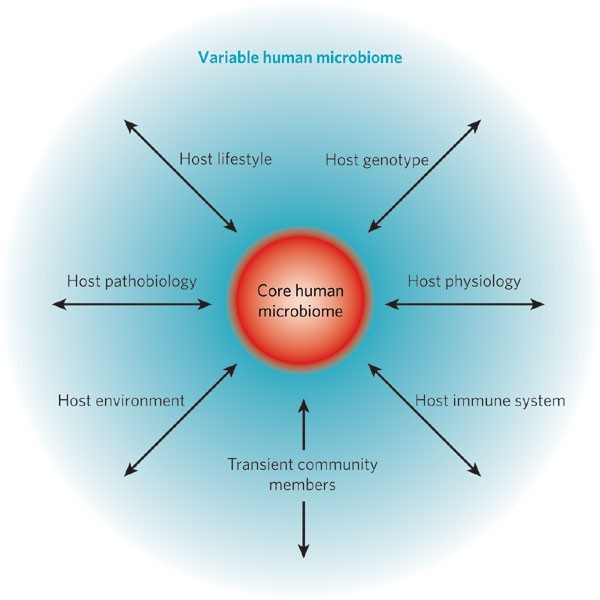
\includegraphics[width=0.5 \linewidth]{figures/microbiome.jpg}
                \caption{Concept of a Core Human Microbiome \protect\cite{microbiome1}}
                \label{fig:microbiome-concept}
            \end{figure}

        \subsection{Ribosomal RNA}
            Ribosomal RNA (rRNA) is well-known as a key to phylogeny \cite{rRNA1}.

        \subsection{16S rRNA Gene Sequencing}

        \subsection{Periodontitis}
            Periodontitis is an inflammatory conditions which effecting periodontium, tissues  which surround and support teeth. Major components of periodontitis are clinical attachment loss and bone loss \cite{periodontitis1}. Previous study found risk factors of periodontitis such as smoking, diabetes, genetic factors and host response \cite{periodontitis2}.

    \section{Materials}
        \subsection{16S rRNA Gene Sequencing}

            \begin{itemize}
                \item 100 Healthy samples
                \item 50 Chronic Early Periodontitis Sample
                \item 50 Chronic Moderate Periodontitis Sample
                \item 50 Chronic Severe Periodontitis Sample
            \end{itemize}

    \section{Methods}
        \subsection{QIIME2 Workflow}
            QIIME2 is a capable, expandable and distributed microbiome analysis package with transparent analysis \cite{qiime1, qiime2}. A theoretic overview of QIIME2 workflow is shown as figure \ref{fig:qiime-workflow}.

            \begin{figure}[p]
                \centering
                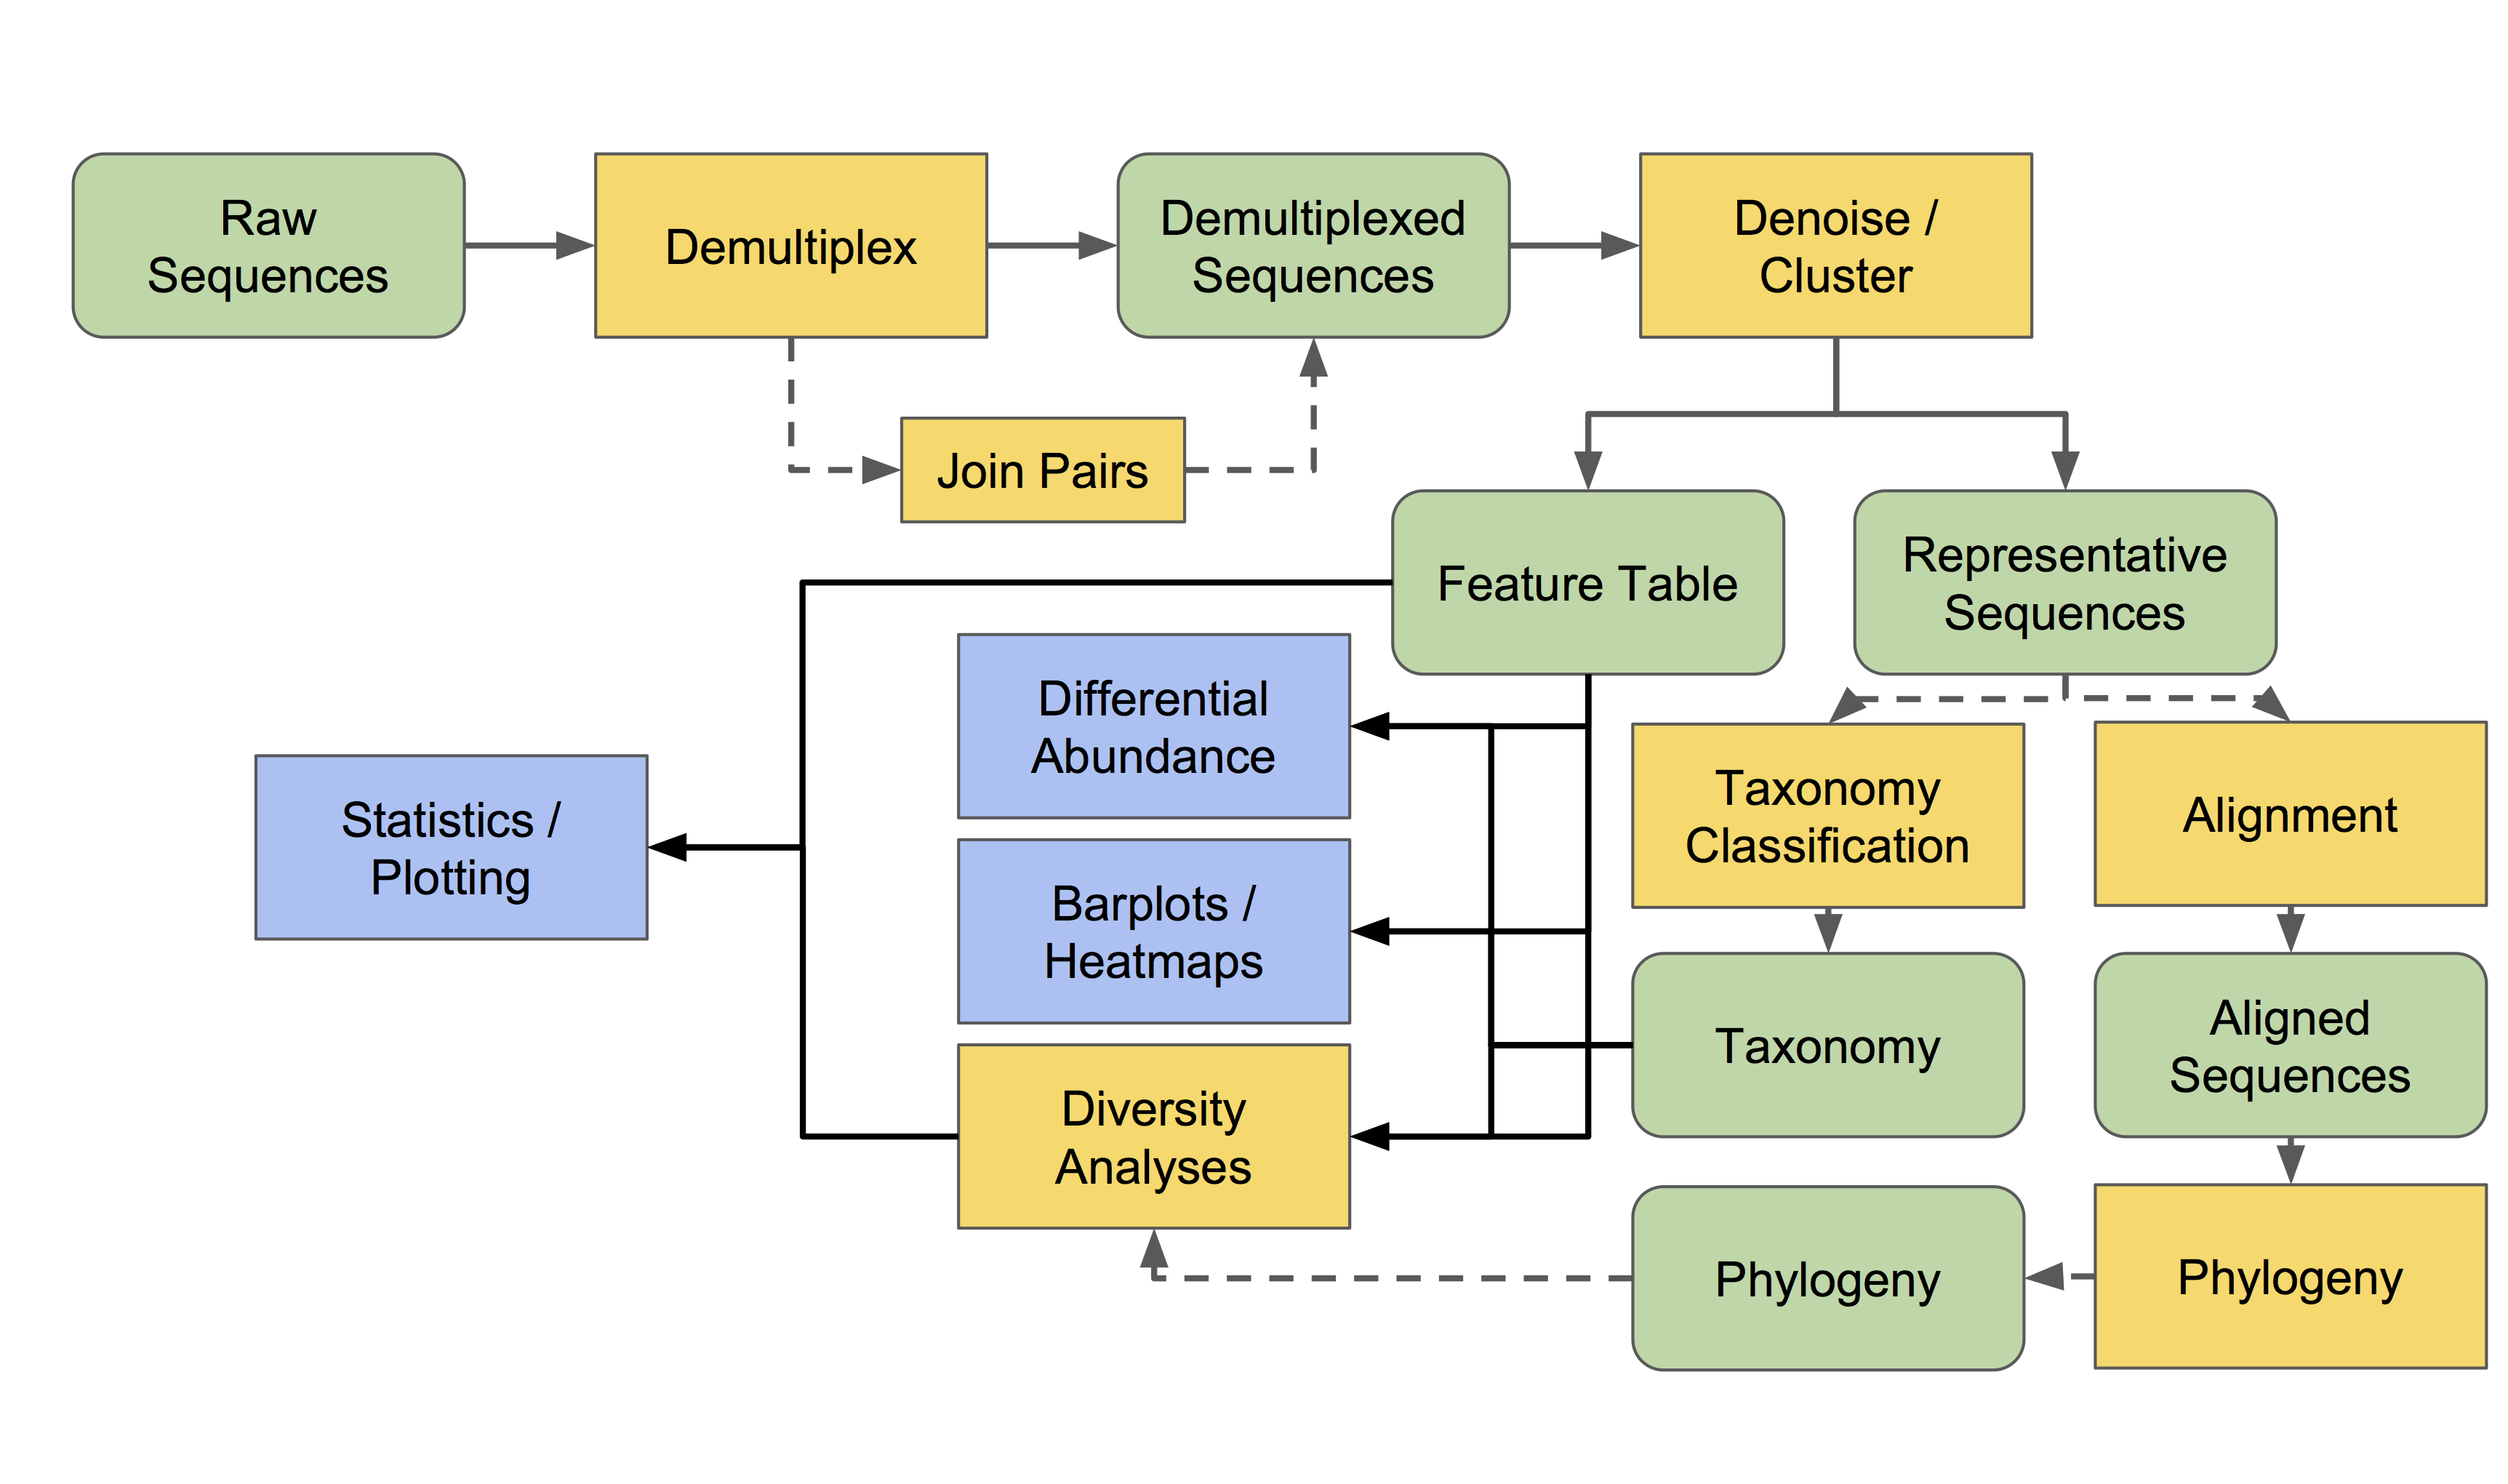
\includegraphics[width=0.8 \linewidth]{figures/qiime.png}
                \caption{A Theoretic Overview of QIIME2 Workflow \protect\cite{qiime1, qiime2}}
                \label{fig:qiime-workflow}
            \end{figure}

            \subsubsection{Denoising techniques}
                There are two denoising techniques provided by QIIME2: DADA2 \cite{DADA1} and Deblur \cite{deblur1}. Major difference between DADA2 and Deblur, as shown as figure \ref{fig:denosing-workflow}, is a strategy, the strategy used to divide as different species. DADA2 uses amplicon sequence variants (ASVs), strictly divides sequences even one-base mismatch. However, Deblur uses operational taxonomic units (OTUs), considers as same sequence when sequences are 97 \% or more matched.

                \begin{figure}[p]
                    \centering
                    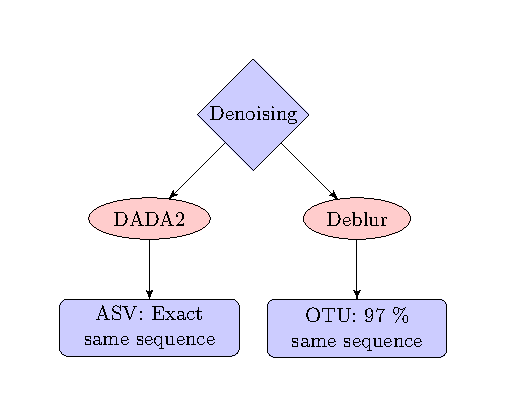
\includegraphics[width=0.5 \linewidth]{figures/denoising/denoising.pdf}
                    \caption{Denoising Techniques which provided by QIIME2}
                    \label{fig:denosing-workflow}
                \end{figure}

            \subsubsection{Taxonomy Classification}
                There are three taxonomy classification databases: Greengenes (GG) \cite{greengenes1}, SILVA \cite{silva1} and Human Oral Microbiome Database (HOMD) \cite{homd1}. Major difference among these databases is resolution. Resolution of GG and HOMD is from kingdom to species; however, resolution of SILVA is from domain to genus. Previous research have found that a higher accuracy at taxonomic levels above genus level; but accuracy drops at species level \cite{performance1}.

                \begin{figure}[p]
                    \centering
                    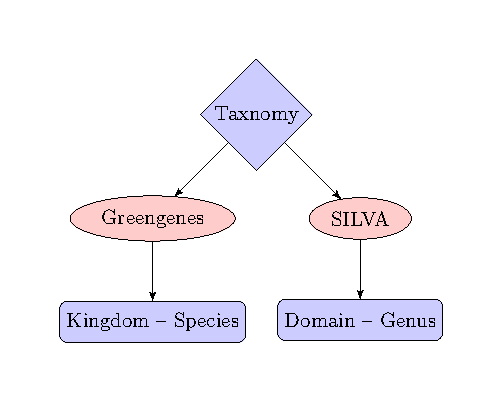
\includegraphics[width=0.5 \linewidth]{figures/taxonomy/taxonomy.pdf}
                    \caption{Taxonomy Classification which provided by QIIME2}
                    \label{fig:taxonomy-workflow}
                \end{figure}

            \subsubsection{Merging Denoising and Taxonomy Classification}
                After denosing and taxonomy classification steps, some different IDs (ASVs or OTUs) have been identified as same taxonomy. In that case, the different IDs will be merged into one taxonomy (Figure \ref{fig:merging}).

                \begin{figure}[p]
                    \centering
                    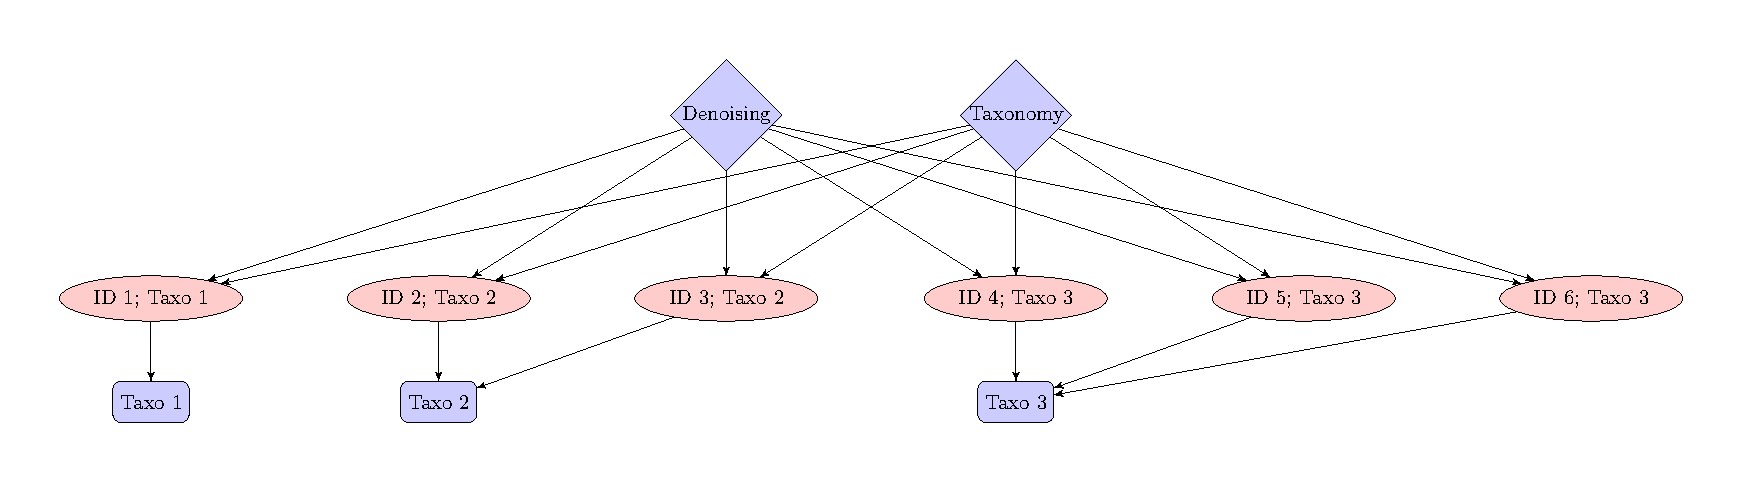
\includegraphics[width=0.8 \linewidth]{figures/Merging/merging.pdf}
                    \caption{Example Diagram for Merging Denoising and Taxonomy Classification}
                    \label{fig:merging}
                \end{figure}

            \subsubsection{Rarefaction}
                Rarefaction is a statistical method of estimating the number of species expected in a random sample which taken from a collection \cite{rarefaction1}. Moreover, rarefaction allows comparisons of the species richness among communities. Thus, rarefaction is a good choice for normalization \cite{rarefaction2}.

            \subsubsection{Alpha-diversity}
                Alpha-diversity is a metric which shows the richness of taxa at a single community. There are four alpha-diversity indices which provided from QIIME2:
                \begin{itemize}
                    \item Evenness index \cite{evenness1}.
                    \item Faith's phylogenetic diversity (Faith PD) \cite{faith1}.
                    \item Observed features.
                    \item Shannon's diversity index \cite{shannon1}.
                \end{itemize}

                Evenness index shows a measurement of diversity in different type at community \cite{evenness1}; Faith's phylogenetic diversity, however, indicates a qualitative measurement of community richness which priorities for species conservation which incorporates with taxic diversity \cite{faith1}. Observed features, as its name, is a number of observed features in microbiome. Moreover, Shannon's diversity index means a significant aspect of community richness \cite{shannon1}.

            \subsubsection{Beta-diversity}
                Beta-diversity is a metric which indicates the taxonomic differentiation between multiple communities. There are four beta-diversity indices which provided from QIIME2:
                \begin{itemize}
                    \item Bray-Curtis distance index \cite{bray1}.
                    \item Jaccard distance index \cite{jaccard1}.
                    \item Unweighted UniFrac distance index \cite{unifrac1}.
                    \item Weighted UniFrac distance index \cite{unifrac1}.
                \end{itemize}

                Bray-Curtis distance index shows a quantitative measurement of community dissimilarity \cite{bray1}; Jaccard distance index, however, indicates a measurement of local distribution among communities. UniFrac distance indices reveal measurements of phylogenetic distances \cite{unifrac1}. Difference between unweighted UniFrac distance index and weighted UniFrac distance index is a qualitative and a quantitative, respectively.

            \subsubsection{ANCOM}
                ANCOM (Analysis of composition of microbiomes) can be used for analyzing the composition of microbiome in multiple populations \cite{ANCOM1}. Example ANCOM volcano plot is shows as figure \ref{fig:ancom-example}. In figure \ref{fig:ancom-example}, two metrics are clearly shown: clr and W. clr stands for centered $\log$ ratio, and W is a count of the number of sub-hypothesis which have passed for given species.

                \begin{figure}[p]
                    \centering
                    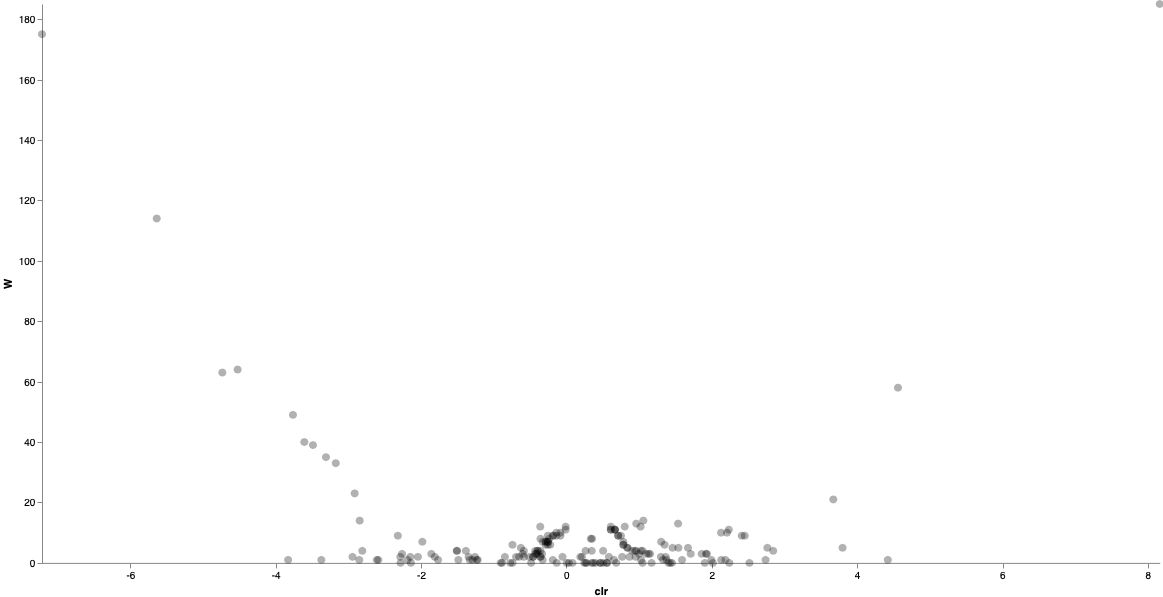
\includegraphics[width=0.8 \linewidth]{figures/ANCOM/example.png}
                    \caption{Example ANCOM Volcano Plot which Provided by QIIME2 \protect\cite{qiime1, qiime2}}
                    \label{fig:ancom-example}
                \end{figure}

        \subsection{Python Packages}
            \subsubsection{Pandas}
                Pandas is a Python package of rich data structures and tools for analyzing with structured data sets \cite{pandas1}.

            \subsubsection{Scikit-learn}
                Scikit-learn grants state-of-the-art implementation of many machine learning algorithms, while controlling an easy-to-use interface tightly integrated the Python code \cite{sklearn1}.

            \subsubsection{Matplotlib}
                Matplotlib is a Python graphics package which used for application development, interactive scripting and publication quality image generation \cite{matplotlib2}. Matplotlib, also, is designed to create simple plots with a few commands \cite{matplotlib1}.

            \subsubsection{Seaborn}
                Seaborn is a Python data visualization package which based on matplotlib, allows a high-level interface for displaying engaging and descriptive statistical graphics \cite{seaborn1}.

        \subsection{t-SNE}
            t-SNE (t-distributed stochastic neighbor embedding) reveals high-dimensional data a location in two-dimensional map \cite{tSNE1}. Figure \ref{fig:tsne-example} is example of t-SNE with hand-writing digits \cite{tSNE1}. In figure \ref{fig:tsne-example}, all 10 digits are grouped into 10 groups clearly; some hand-writings, however, are classified into wrong groups due to their similar shapes, such as 0 and 6.

            \begin{figure}[p]
                \centering
                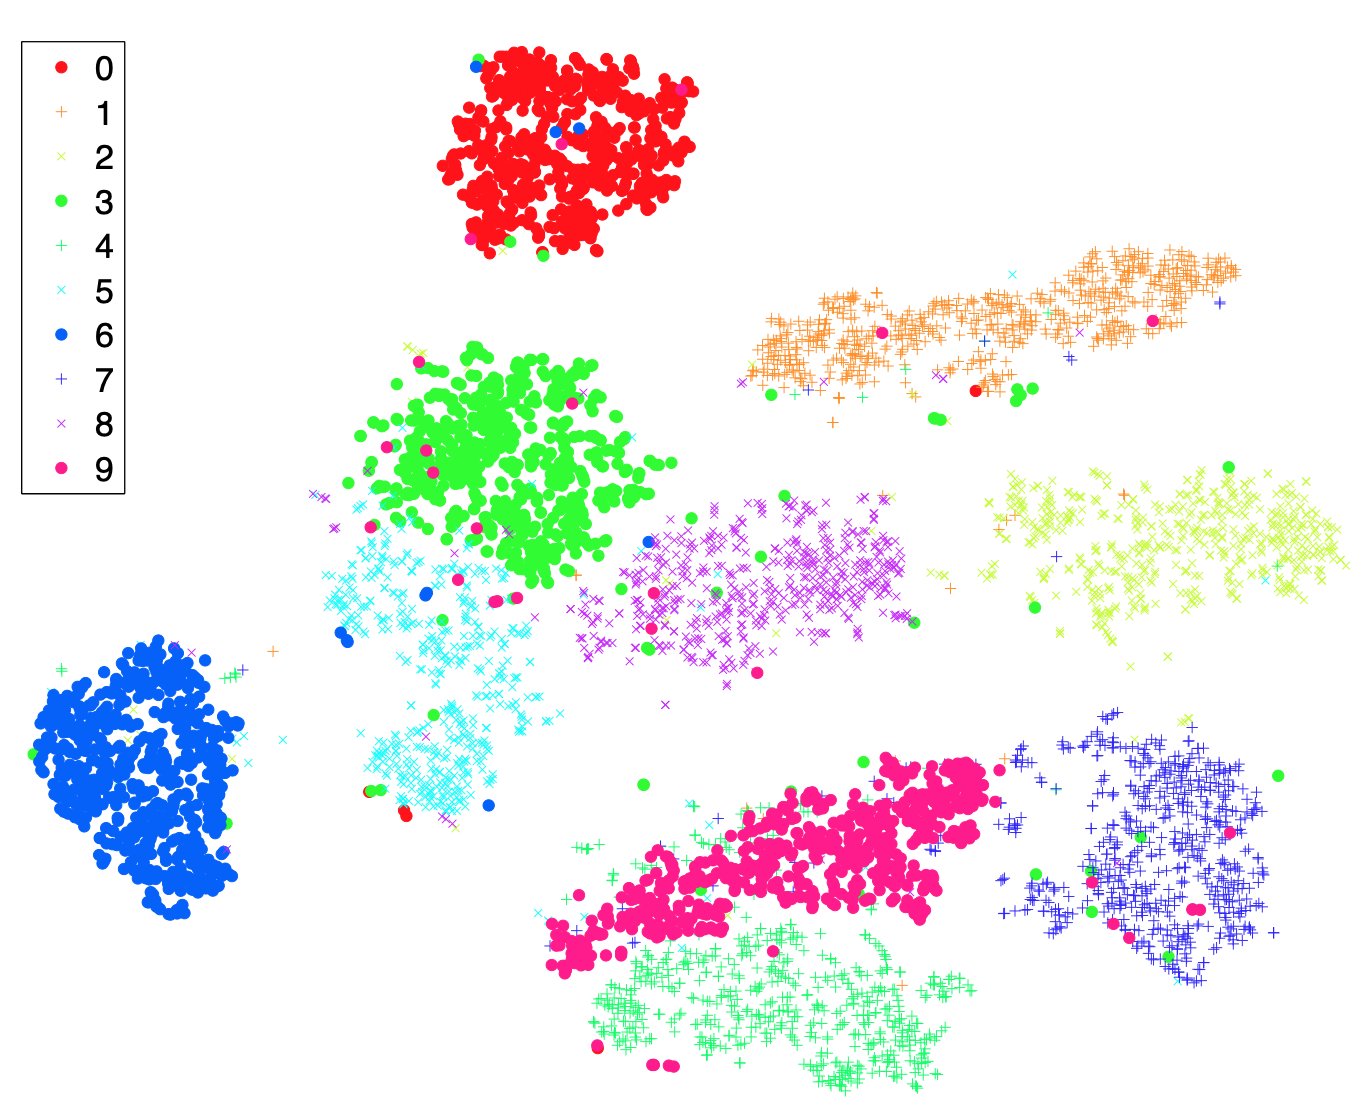
\includegraphics[width=0.4 \linewidth]{figures/tSNE.png}
                \caption{Visualization by t-SNE \protect\cite{tSNE1}}
                \label{fig:tsne-example}
            \end{figure}

        \subsection{Classification}
            In machine learning, Classification is one of supervised learning which identifies a class of a new observation, depends on given information which consist of training observations and their classes.

            In this study, classification will be carried out as figure \ref{fig:classification}; and the third step in figure \ref{fig:classification} is demonstrated in minute detail as figure \ref{fig:deciding-best}. Note that the first step in figure \ref{fig:classification} is optional: due to tables herein-after, such as table\ref{tb:alpha-evenness-dada2}, show that no statistically significant differences between healthy samples and early periodontitis samples and between moderate periodontitis samples and severe periodontitis samples.

            Moreover, evaluations of classification algorithm are carried out with derivations from confusion matrix (table \ref{tb:confusion-matrix}):

            \begin{itemize}
                \item Accuracy (ACC) $ = \frac{TP + TN}{TP + TN + FP + FN}$
                \item Balanced Accuracy (BA) $ = \frac{TP}{2 \times (TP + FN)} + \frac{TN}{2 \times (TN + FP)}$
                \item Sensitivity (SEN) $ = \frac{TP}{TP + FN}$
                \item Specificity (SPE) $ = \frac{TN}{TN + FP}$
                \item Precision (PRE) $ = \frac{TP}{TP + FP}$
            \end{itemize}

            \begin{table}[p]
                \centering
                \caption{Confusion Matrix}
                \label{tb:confusion-matrix}
                \begin{tabular}{c|c|cc}
                    \multicolumn{2}{c|}{\multirow{2}{*}{}} & \multicolumn{2}{c}{Actual Class} \\ \cline{3-4}
                    \multicolumn{2}{c|}{} & Positive & Negative \\ \hline
                    \multirow{2}{*}{Predicted Class} & Positive & True Positive (TP) & False Positive (FP) \\
                    & Negative & False Negative (FN) & True Negative (TN)
                \end{tabular}
            \end{table}

            \begin{figure}[p]
                \centering
                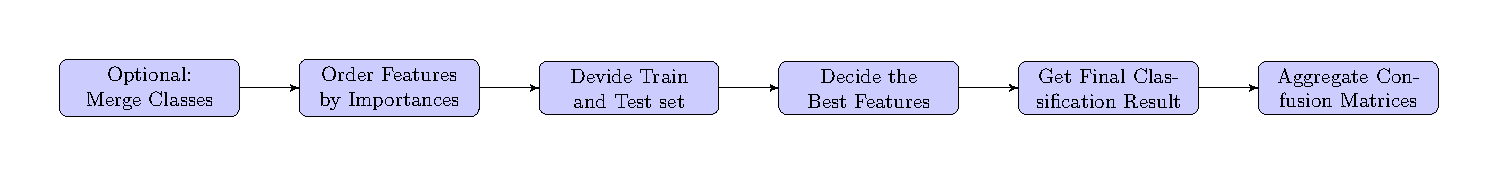
\includegraphics[width=0.8 \linewidth]{figures/Classifier/classifier.pdf}
                \caption{Workflow of Classification}
                \label{fig:classification}
            \end{figure}

            \begin{figure}[p]
                \centering
                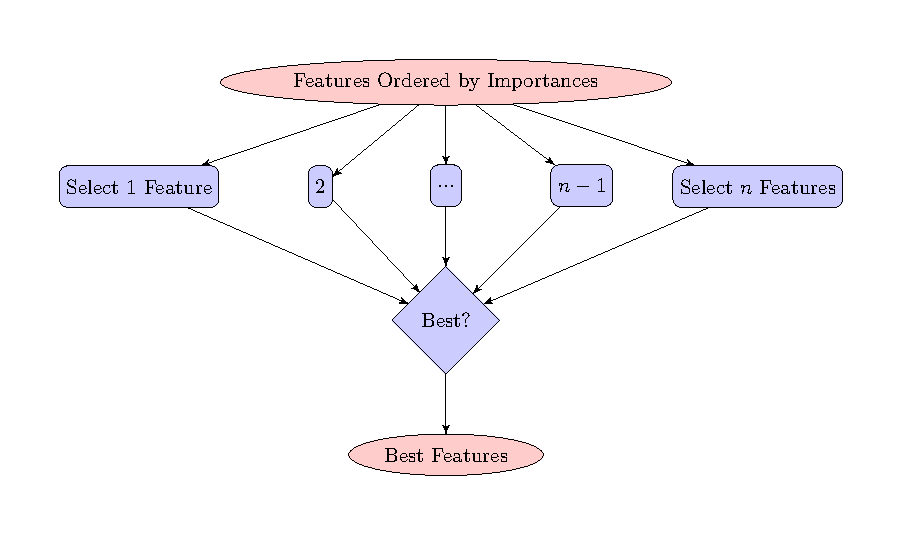
\includegraphics[width=0.6 \linewidth]{figures/Classifier/best.pdf}
                \caption{Deciding the Best Features}
                \label{fig:deciding-best}
            \end{figure}

            \subsubsection{Random Forest Classification}
                As figure \ref{fig:classification}, importance of features have to be derived by classifier. Random Forest classifier \cite{RandomForest1} can get this information, and is used frequently by researchers. Hence, Random Forest classifier will be carried out with every class (Figure \ref{fig:RF-whole-workflow}) or with merged classes (Figure \ref{fig:RF-merging-workflow}).

                \begin{figure}[p]
                    \centering
                    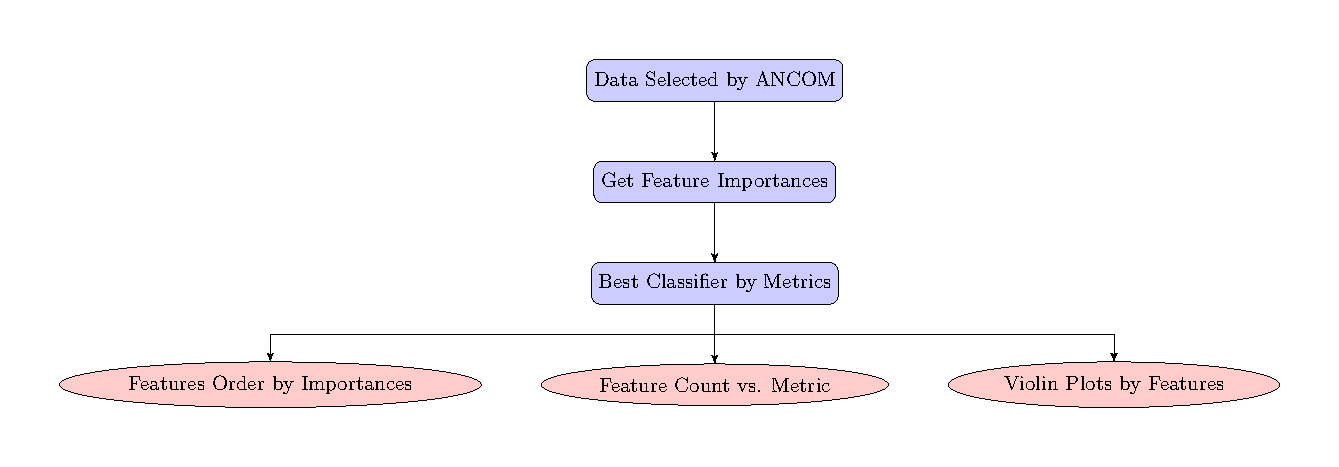
\includegraphics[width=0.6 \linewidth]{figures/RandomForest/whole.pdf}
                    \caption{Random Forest Classifier Workflow}
                    \label{fig:RF-whole-workflow}
                \end{figure}

                \begin{figure}[p]
                    \centering
                    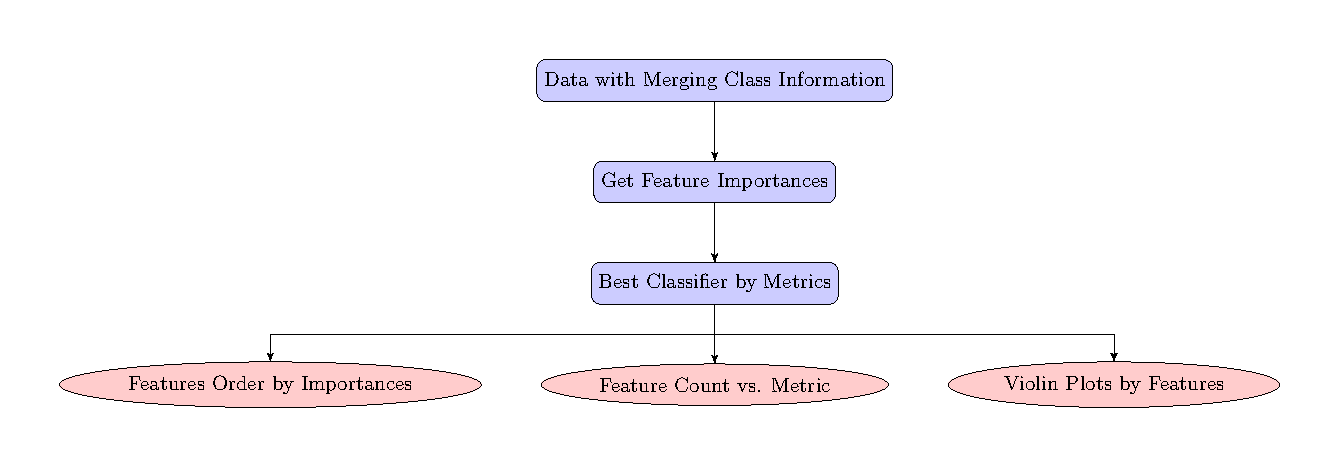
\includegraphics[width=0.6 \linewidth]{figures/RandomForest/merge.pdf}
                    \caption{Random Forest Classifier Workflow with Merging}
                    \label{fig:RF-merging-workflow}
                \end{figure}

    \section{Results}
        \subsection{Quality Filter}
            Longer sequences have more fallen sequence quality than shorter. Thus, sequences which longer than threshold should be trimmed out due to their low quality. However, gold-standard strategy for deciding the threshold does not exist; the threshold is set as longest sequence length which have half of sequences have greater than 30 quality score. Hence, sequence quality plot is shown as figure \ref{fig:sequence-quality}; trimmed length in forward reads is 300, and trimmed length in reverse reads is 265.

            \begin{figure}[p]
                \centering
                $\begin{array}{cc}
                    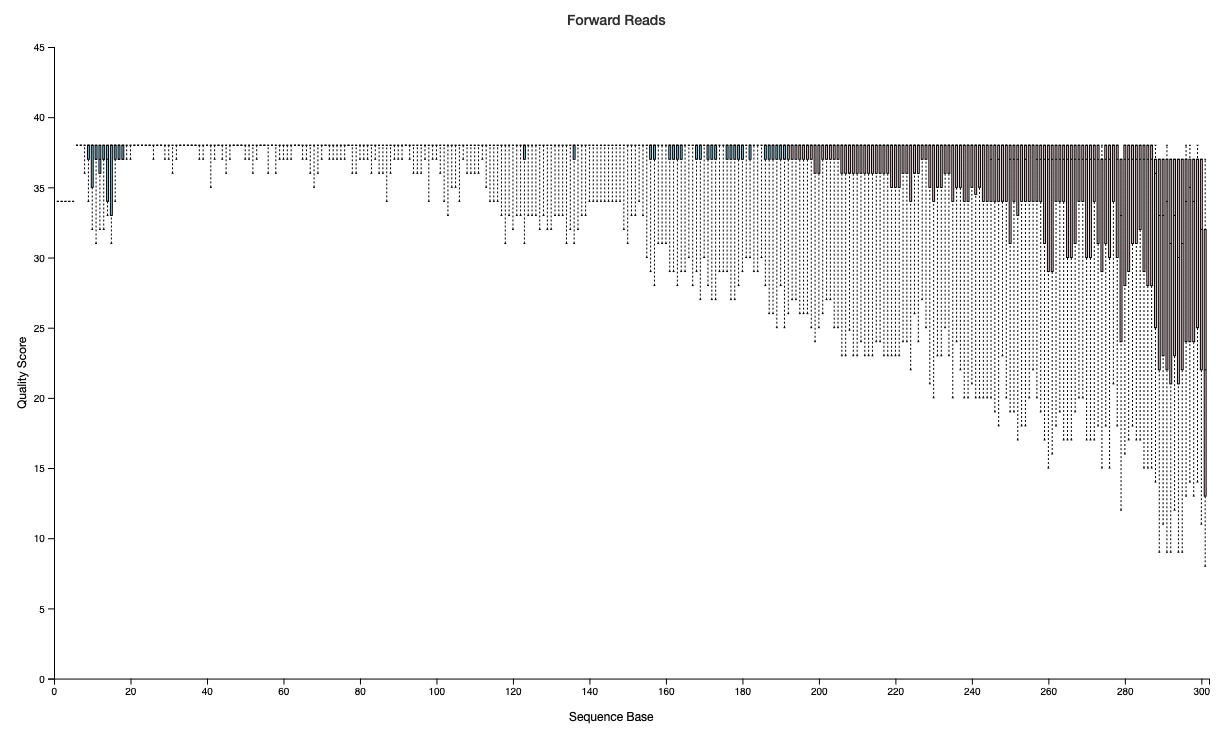
\includegraphics[width=0.4 \linewidth]{figures/QualityFilter/Forward.png}
                    &
                    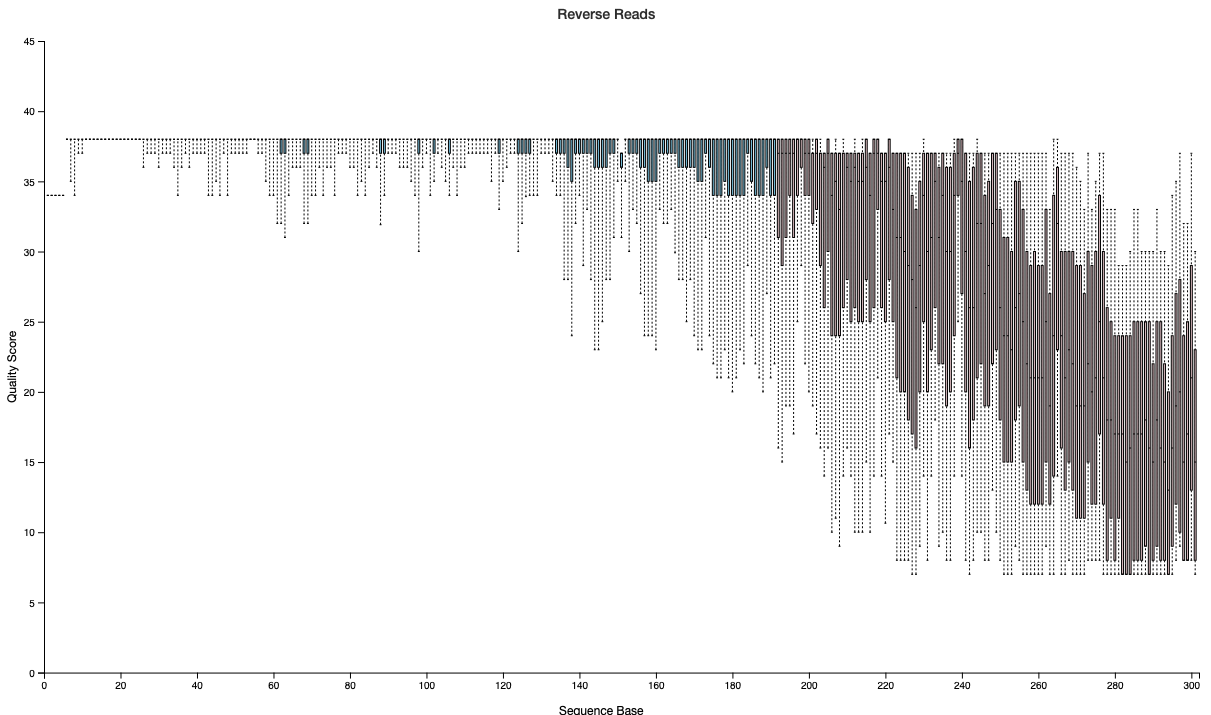
\includegraphics[width=0.4 \linewidth]{figures/QualityFilter/Reverse.png}
                    \\
                    \mbox{(a) Forward Reads} & \mbox{(b) Reverse Reads} \\
                \end{array}$
                \caption{Sequence Quality Plot}
                \label{fig:sequence-quality}
            \end{figure}

        \subsection{Rarefaction}
            Sampling depth should be decided for rarefaction. Gold-standard method for determining sampling depth is minimum frequency in the samples. Hence, sampling depth with DADA2 is 3,786 (Figure \ref{fig:frequency-sample-dada2}), and sampling depth with Deblur is 7,253 (Figure \ref{fig:frequency-sample-deblur}).

            \begin{figure}[p]
                \centering
                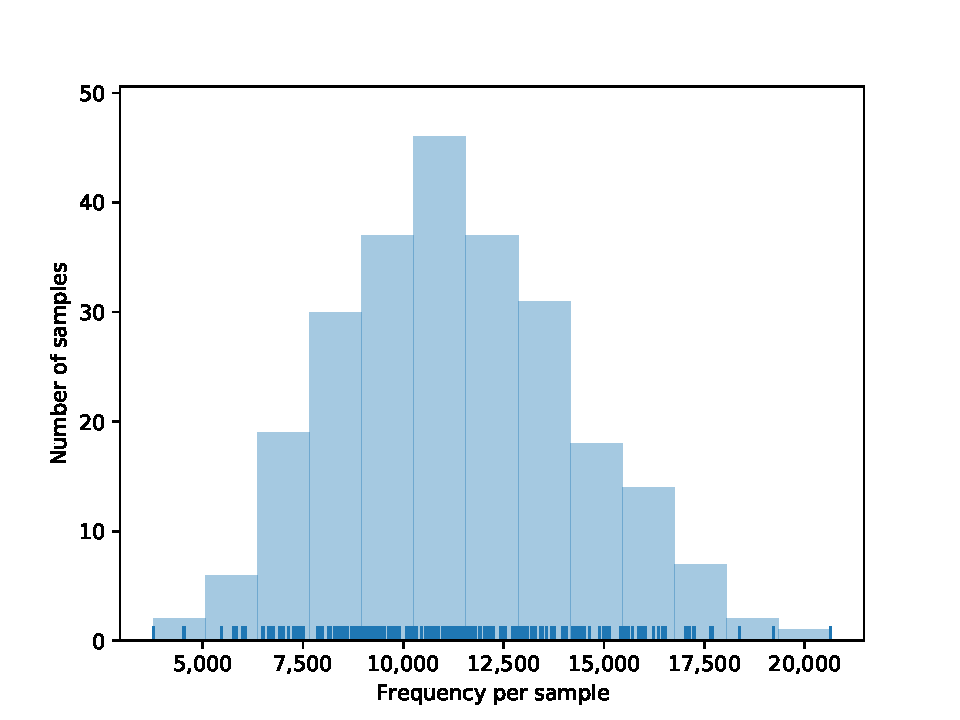
\includegraphics[width=0.6 \linewidth]{figures/Rarefaction/DADA.pdf}
                \caption{Frequency and Number per Sample by DADA2}
                \label{fig:frequency-sample-dada2}
            \end{figure}

            \begin{figure}[p]
                \centering
                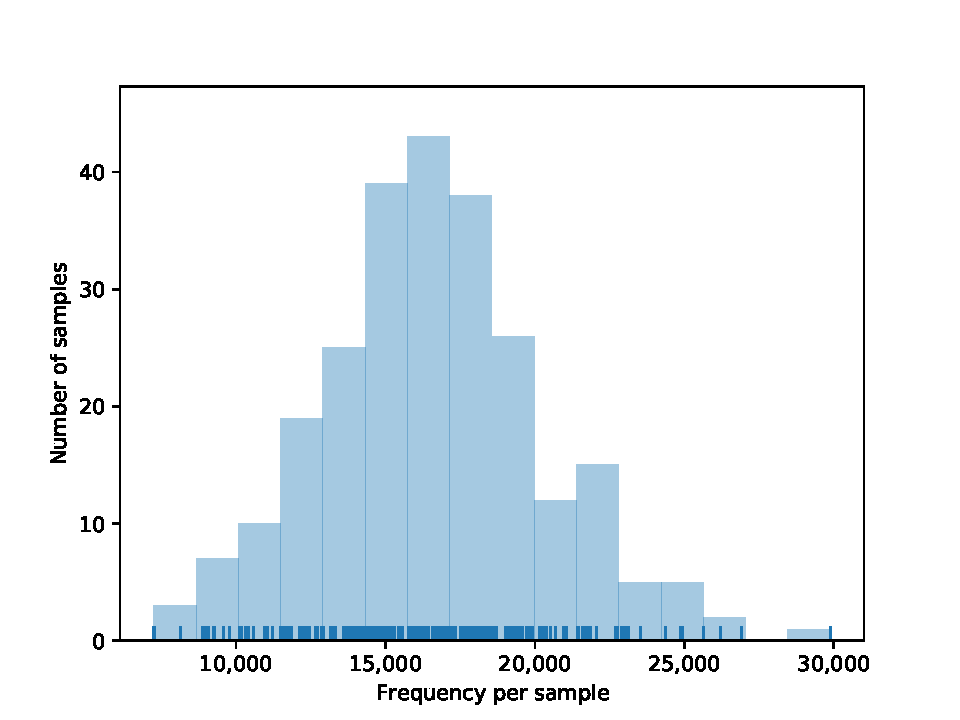
\includegraphics[width=0.6 \linewidth]{figures/Rarefaction/Deblur.pdf}
                \caption{Frequency and Number per Sample by Deblur}
                \label{fig:frequency-sample-deblur}
            \end{figure}

        \subsection{Alpha-diversity}
            Alpha-diversity analysis with DADA2 was done: Evenness index (Table \ref{tb:alpha-evenness-dada2} and Figure \ref{fig:evenness-dada2}), Faith PD (Table \ref{tb:alpha-faith-dada2} and Figure \ref{fig:faith-dada2}), observed feature index (Table \ref{tb:alpha-observed-dada2} and Figure \ref{fig:observed-dada2}) and Shannon's diversity index (Table \ref{tb:alpha-shannon-dada2} and Figure \ref{fig:shannon-dada2}). Also, alpha-diversity analysis with DADA2 was done: Evenness index (Table \ref{tb:alpha-evenness-deblur} and Figure \ref{fig:evenness-deblur}), Faith PD (Table \ref{tb:alpha-faith-deblur} and Figure \ref{fig:faith-deblur}), observed feature index (Table \ref{tb:alpha-observed-deblur} and Figure \ref{fig:observed-deblur}) and Shannon's diversity index (Table \ref{tb:alpha-shannon-deblur} and Figure \ref{fig:shannon-deblur}). Moreover, Kruskal-Wallis tests among all groups are shown as table \ref{tb:alpha-all-dada2} (with DADA2) and table \ref{tb:alpha-all-deblur} (with Deblur).

            \begin{table}[p]
                \centering
                \caption{Kruskal-Wallis Tests among All Group with DADA2}
                \label{tb:alpha-all-dada2}
                \csvautobooktabular{csv/AlphaDiversity/DADA2/all.csv}
            \end{table}

            \begin{table}[p]
                \centering
                \caption{Kruskal-Wallis Tests from Evenness Index with DADA2}
                \label{tb:alpha-evenness-dada2}
                \csvautobooktabular{csv/AlphaDiversity/DADA2/evenness.csv}
            \end{table}

            \begin{table}[p]
                \centering
                \caption{Kruskal-Wallis Tests from Faith PD Index with DADA2}
                \label{tb:alpha-faith-dada2}
                \csvautobooktabular{csv/AlphaDiversity/DADA2/faith.csv}
            \end{table}

            \begin{table}[p]
                \centering
                \caption{Kruskal-Wallis Tests from Observed Features Index with DADA2}
                \label{tb:alpha-observed-dada2}
                \csvautobooktabular{csv/AlphaDiversity/DADA2/observed.csv}
            \end{table}

            \begin{table}[p]
                \centering
                \caption{Kruskal-Wallis Tests from Shannon's Diversity Index with DADA2}
                \label{tb:alpha-shannon-dada2}
                \csvautobooktabular{csv/AlphaDiversity/DADA2/shannon.csv}
            \end{table}

            \begin{figure}[p]
                \centering
                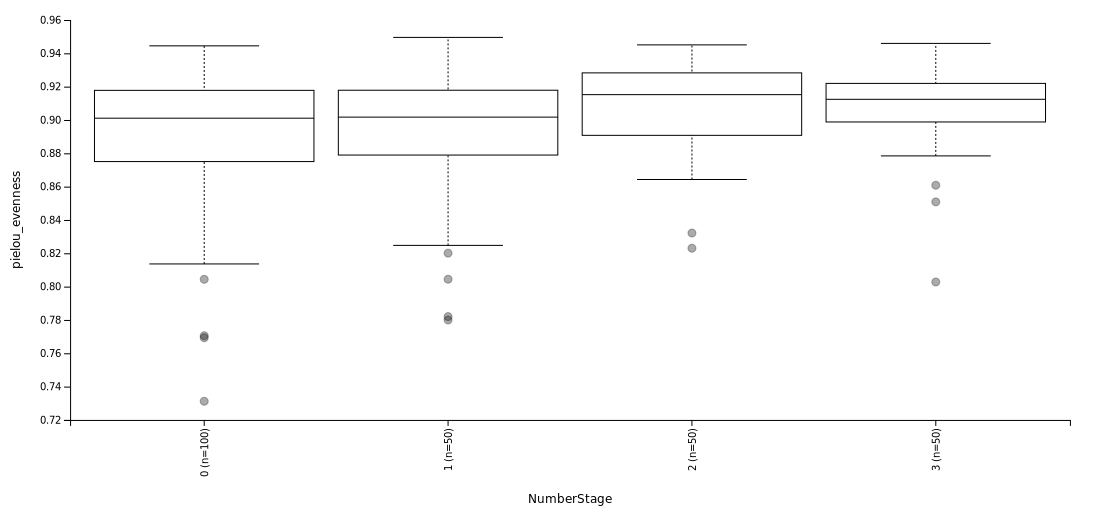
\includegraphics[width=0.8 \linewidth]{figures/AlphaDiversity/DADA2/evenness.png}
                \caption{Evenness Index from DADA2}
                \label{fig:evenness-dada2}
            \end{figure}

            \begin{figure}[p]
                \centering
                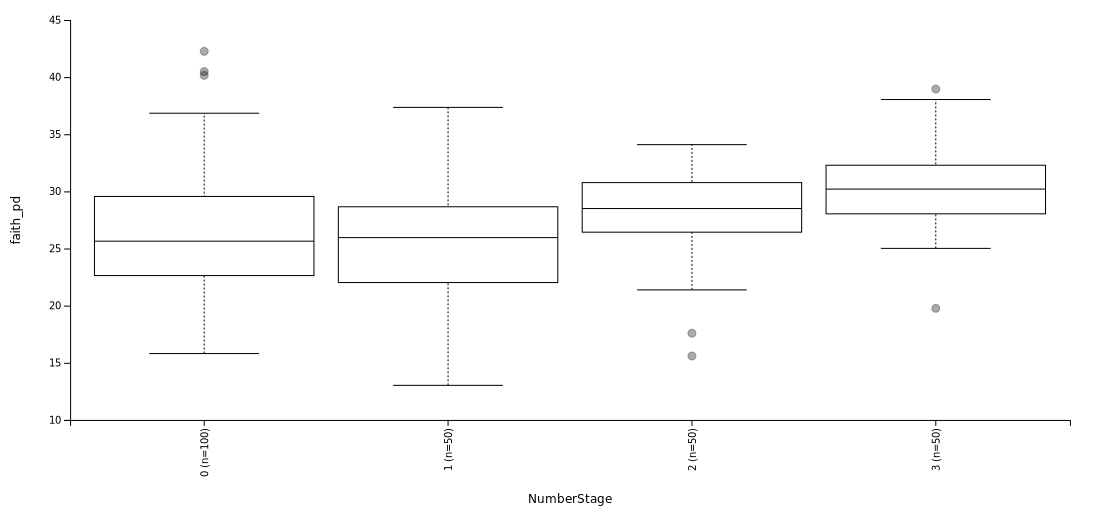
\includegraphics[width=0.8 \linewidth]{figures/AlphaDiversity/DADA2/faith.png}
                \caption{Faith PD Index from DADA2}
                \label{fig:faith-dada2}
            \end{figure}

            \begin{figure}[p]
                \centering
                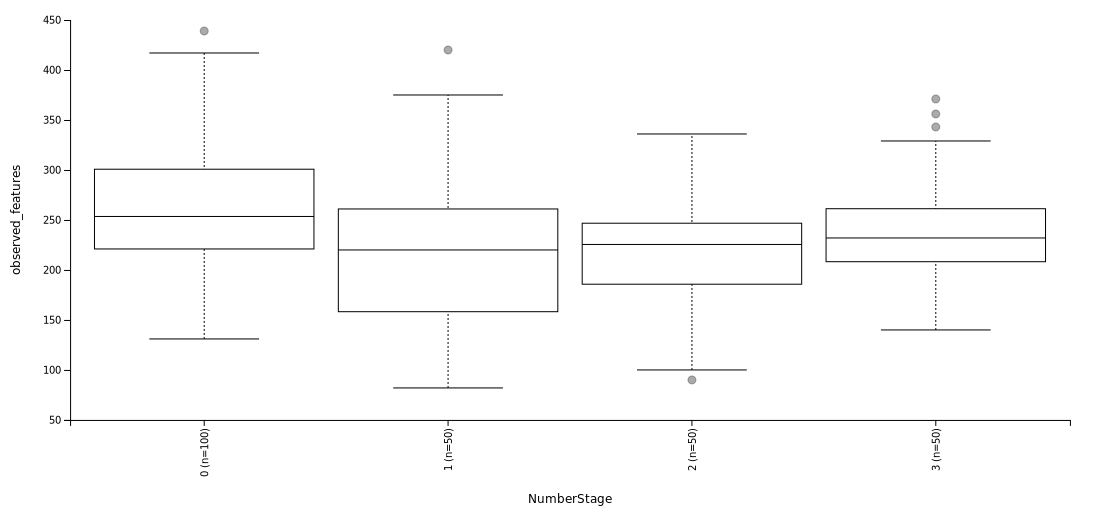
\includegraphics[width=0.8 \linewidth]{figures/AlphaDiversity/DADA2/observed.png}
                \caption{Observed Features Index from DADA2}
                \label{fig:observed-dada2}
            \end{figure}

            \begin{figure}[p]
                \centering
                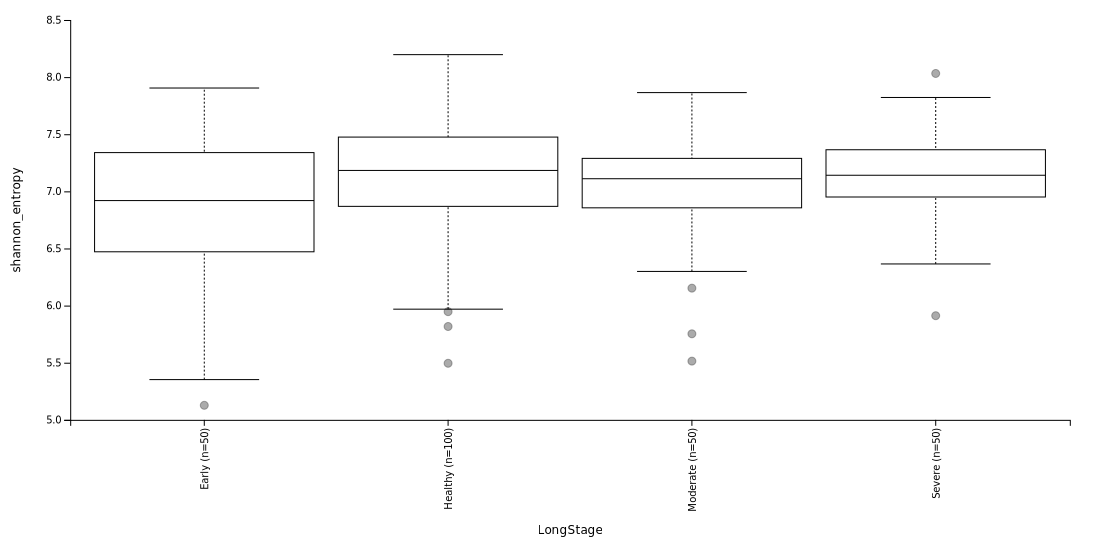
\includegraphics[width=0.8 \linewidth]{figures/AlphaDiversity/DADA2/shannon.png}
                \caption{Shannon's Diversity Index from DADA2}
                \label{fig:shannon-dada2}
            \end{figure}

            \begin{table}[p]
                \centering
                \caption{Kruskal-Wallis Tests among All Group with Deblur}
                \label{tb:alpha-all-deblur}
                \csvautobooktabular{csv/AlphaDiversity/Deblur/all.csv}
            \end{table}

            \begin{table}[p]
                \centering
                \caption{Kruskal-Wallis Tests from Evenness Index with Deblur}
                \label{tb:alpha-evenness-deblur}
                \csvautobooktabular{csv/AlphaDiversity/Deblur/evenness.csv}
            \end{table}

            \begin{table}[p]
                \centering
                \caption{Kruskal-Wallis Tests from Faith PD Index with Deblur}
                \label{tb:alpha-faith-deblur}
                \csvautobooktabular{csv/AlphaDiversity/Deblur/faith.csv}
            \end{table}

            \begin{table}[p]
                \centering
                \caption{Kruskal-Wallis Tests from Observed Features Index with Deblur}
                \label{tb:alpha-observed-deblur}
                \csvautobooktabular{csv/AlphaDiversity/Deblur/observed.csv}
            \end{table}

            \begin{table}[p]
                \centering
                \caption{Kruskal-Wallis Tests from Shannon's Diversity Index with Deblur}
                \label{tb:alpha-shannon-deblur}
                \csvautobooktabular{csv/AlphaDiversity/Deblur/shannon.csv}
            \end{table}

            \begin{figure}[p]
                \centering
                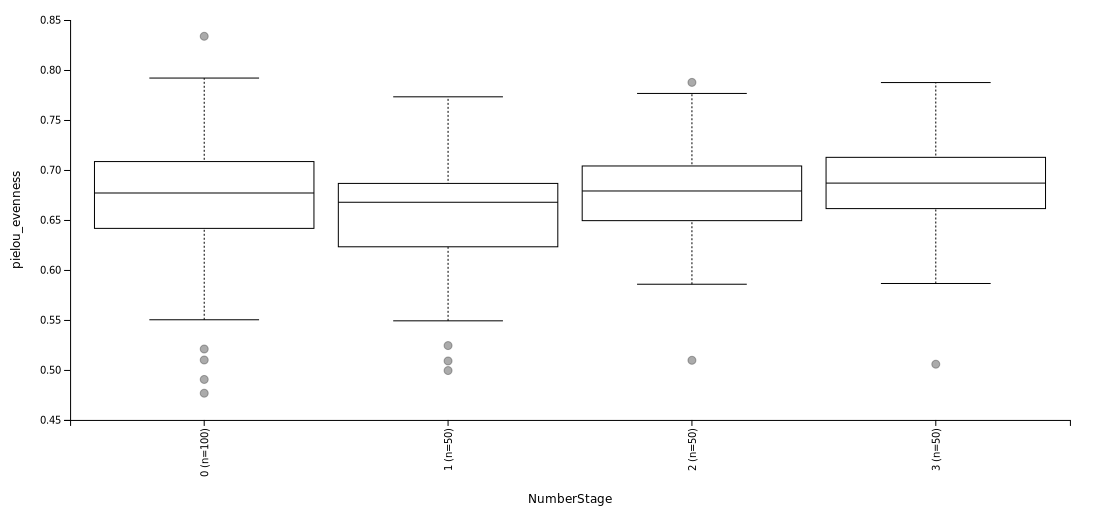
\includegraphics[width=0.8 \linewidth]{figures/AlphaDiversity/Deblur/evenness.png}
                \caption{Evenness Index from Deblur}
                \label{fig:evenness-deblur}
            \end{figure}

            \begin{figure}[p]
                \centering
                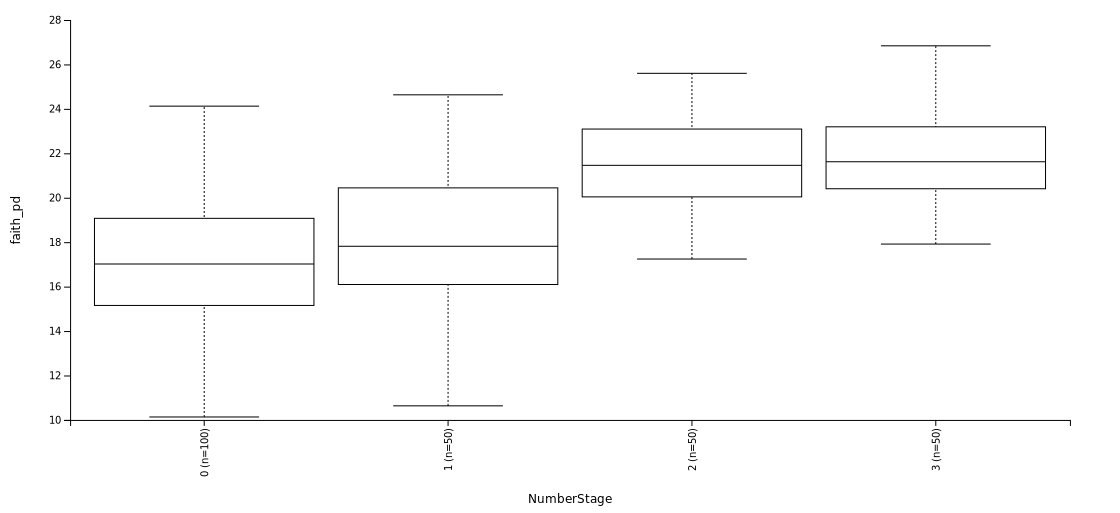
\includegraphics[width=0.8 \linewidth]{figures/AlphaDiversity/Deblur/faith.png}
                \caption{Faith PD Index from Deblur}
                \label{fig:faith-deblur}
            \end{figure}

            \begin{figure}[p]
                \centering
                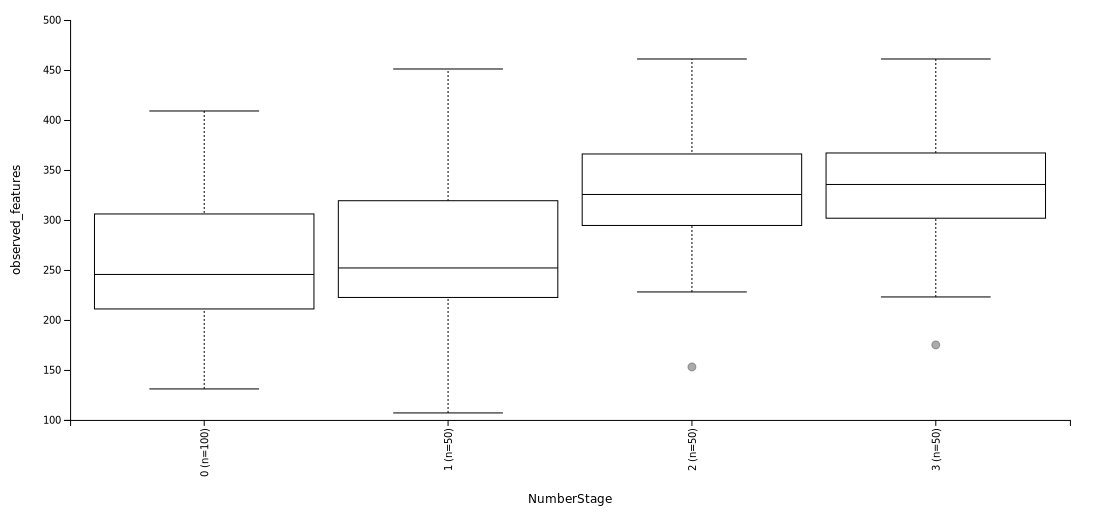
\includegraphics[width=0.8 \linewidth]{figures/AlphaDiversity/Deblur/observed.png}
                \caption{Observed Features Index from Deblur}
                \label{fig:observed-deblur}
            \end{figure}

            \begin{figure}[p]
                \centering
                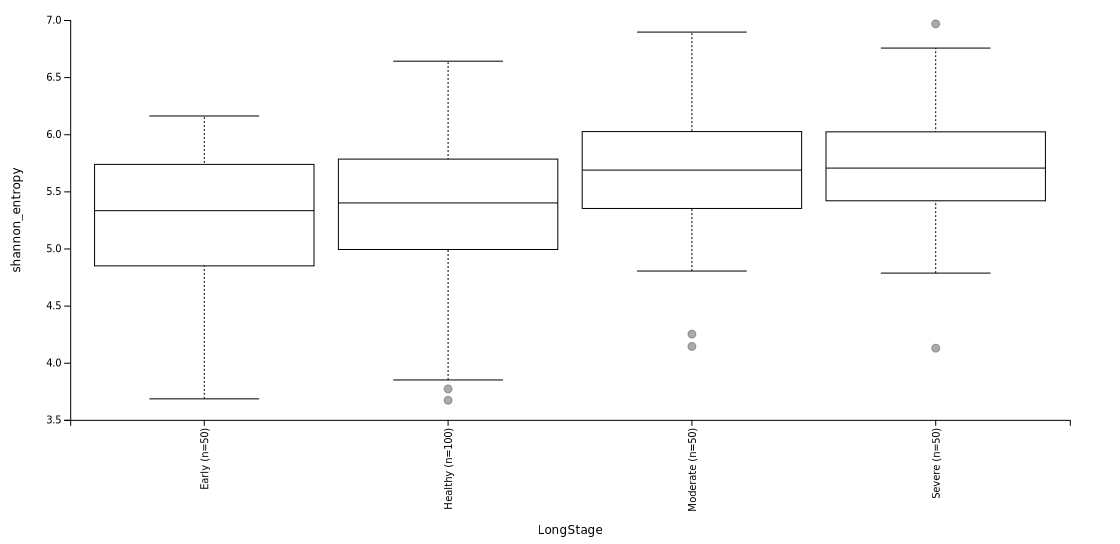
\includegraphics[width=0.8 \linewidth]{figures/AlphaDiversity/Deblur/shannon.png}
                \caption{Shannon's Diversity Index from Deblur}
                \label{fig:shannon-deblur}
            \end{figure}

        \subsection{Beta-diversity}
            Beta-diversity analysis with DADA2 was done: Bray-Curtis distance (Table \ref{tb:bray-dada2} and Figure \ref{fig:bray-dada2}), Jaccard distance (Table \ref{tb:jaccard-dada2} and Figure \ref{fig:jaccard-dada2}), unweighted UniFrac distance (Table \ref{tb:unweighted-dada2} and Figure \ref{fig:unweighted-dada2}) and weighted UniFrac distance (Table \ref{tb:weighted-dada2} and Figure \ref{fig:unweighted-dada2}). Also, beta-diversity analysis with Deblur was done: Bray-Curtis distance (Table \ref{tb:bray-deblur} and Figure \ref{fig:bray-deblur}), Jaccard distance (Table \ref{tb:jaccard-deblur} and Figure \ref{fig:jaccard-deblur}), unweighted UniFrac distance (Table \ref{tb:unweighted-deblur} and Figure \ref{fig:unweighted-deblur}) and weighted UniFrac distance (Table \ref{tb:weighted-deblur} and Figure \ref{fig:unweighted-deblur}).

            \begin{table}[p]
                \centering
                \caption{Bray-Curtis Distance Index with DADA2}
                \label{tb:bray-dada2}
                \csvautobooktabular{csv/BetaDiversity/DADA2/Bray.csv}
            \end{table}

            \begin{table}[p]
                \centering
                \caption{Jaccard Distance Index with DADA2}
                \label{tb:jaccard-dada2}
                \csvautobooktabular{csv/BetaDiversity/DADA2/Jaccard.csv}
            \end{table}

            \begin{table}[p]
                \centering
                \caption{Unweighted UniFrac Distance Index with DADA2}
                \label{tb:unweighted-dada2}
                \csvautobooktabular{csv/BetaDiversity/DADA2/UnweightedUniFrac.csv}
            \end{table}

            \begin{table}[p]
                \centering
                \caption{Weighted UniFrac Distance Index with DADA2}
                \label{tb:weighted-dada2}
                \csvautobooktabular{csv/BetaDiversity/DADA2/WeightedUniFrac.csv}
            \end{table}

            \begin{figure}[p]
                \centering
                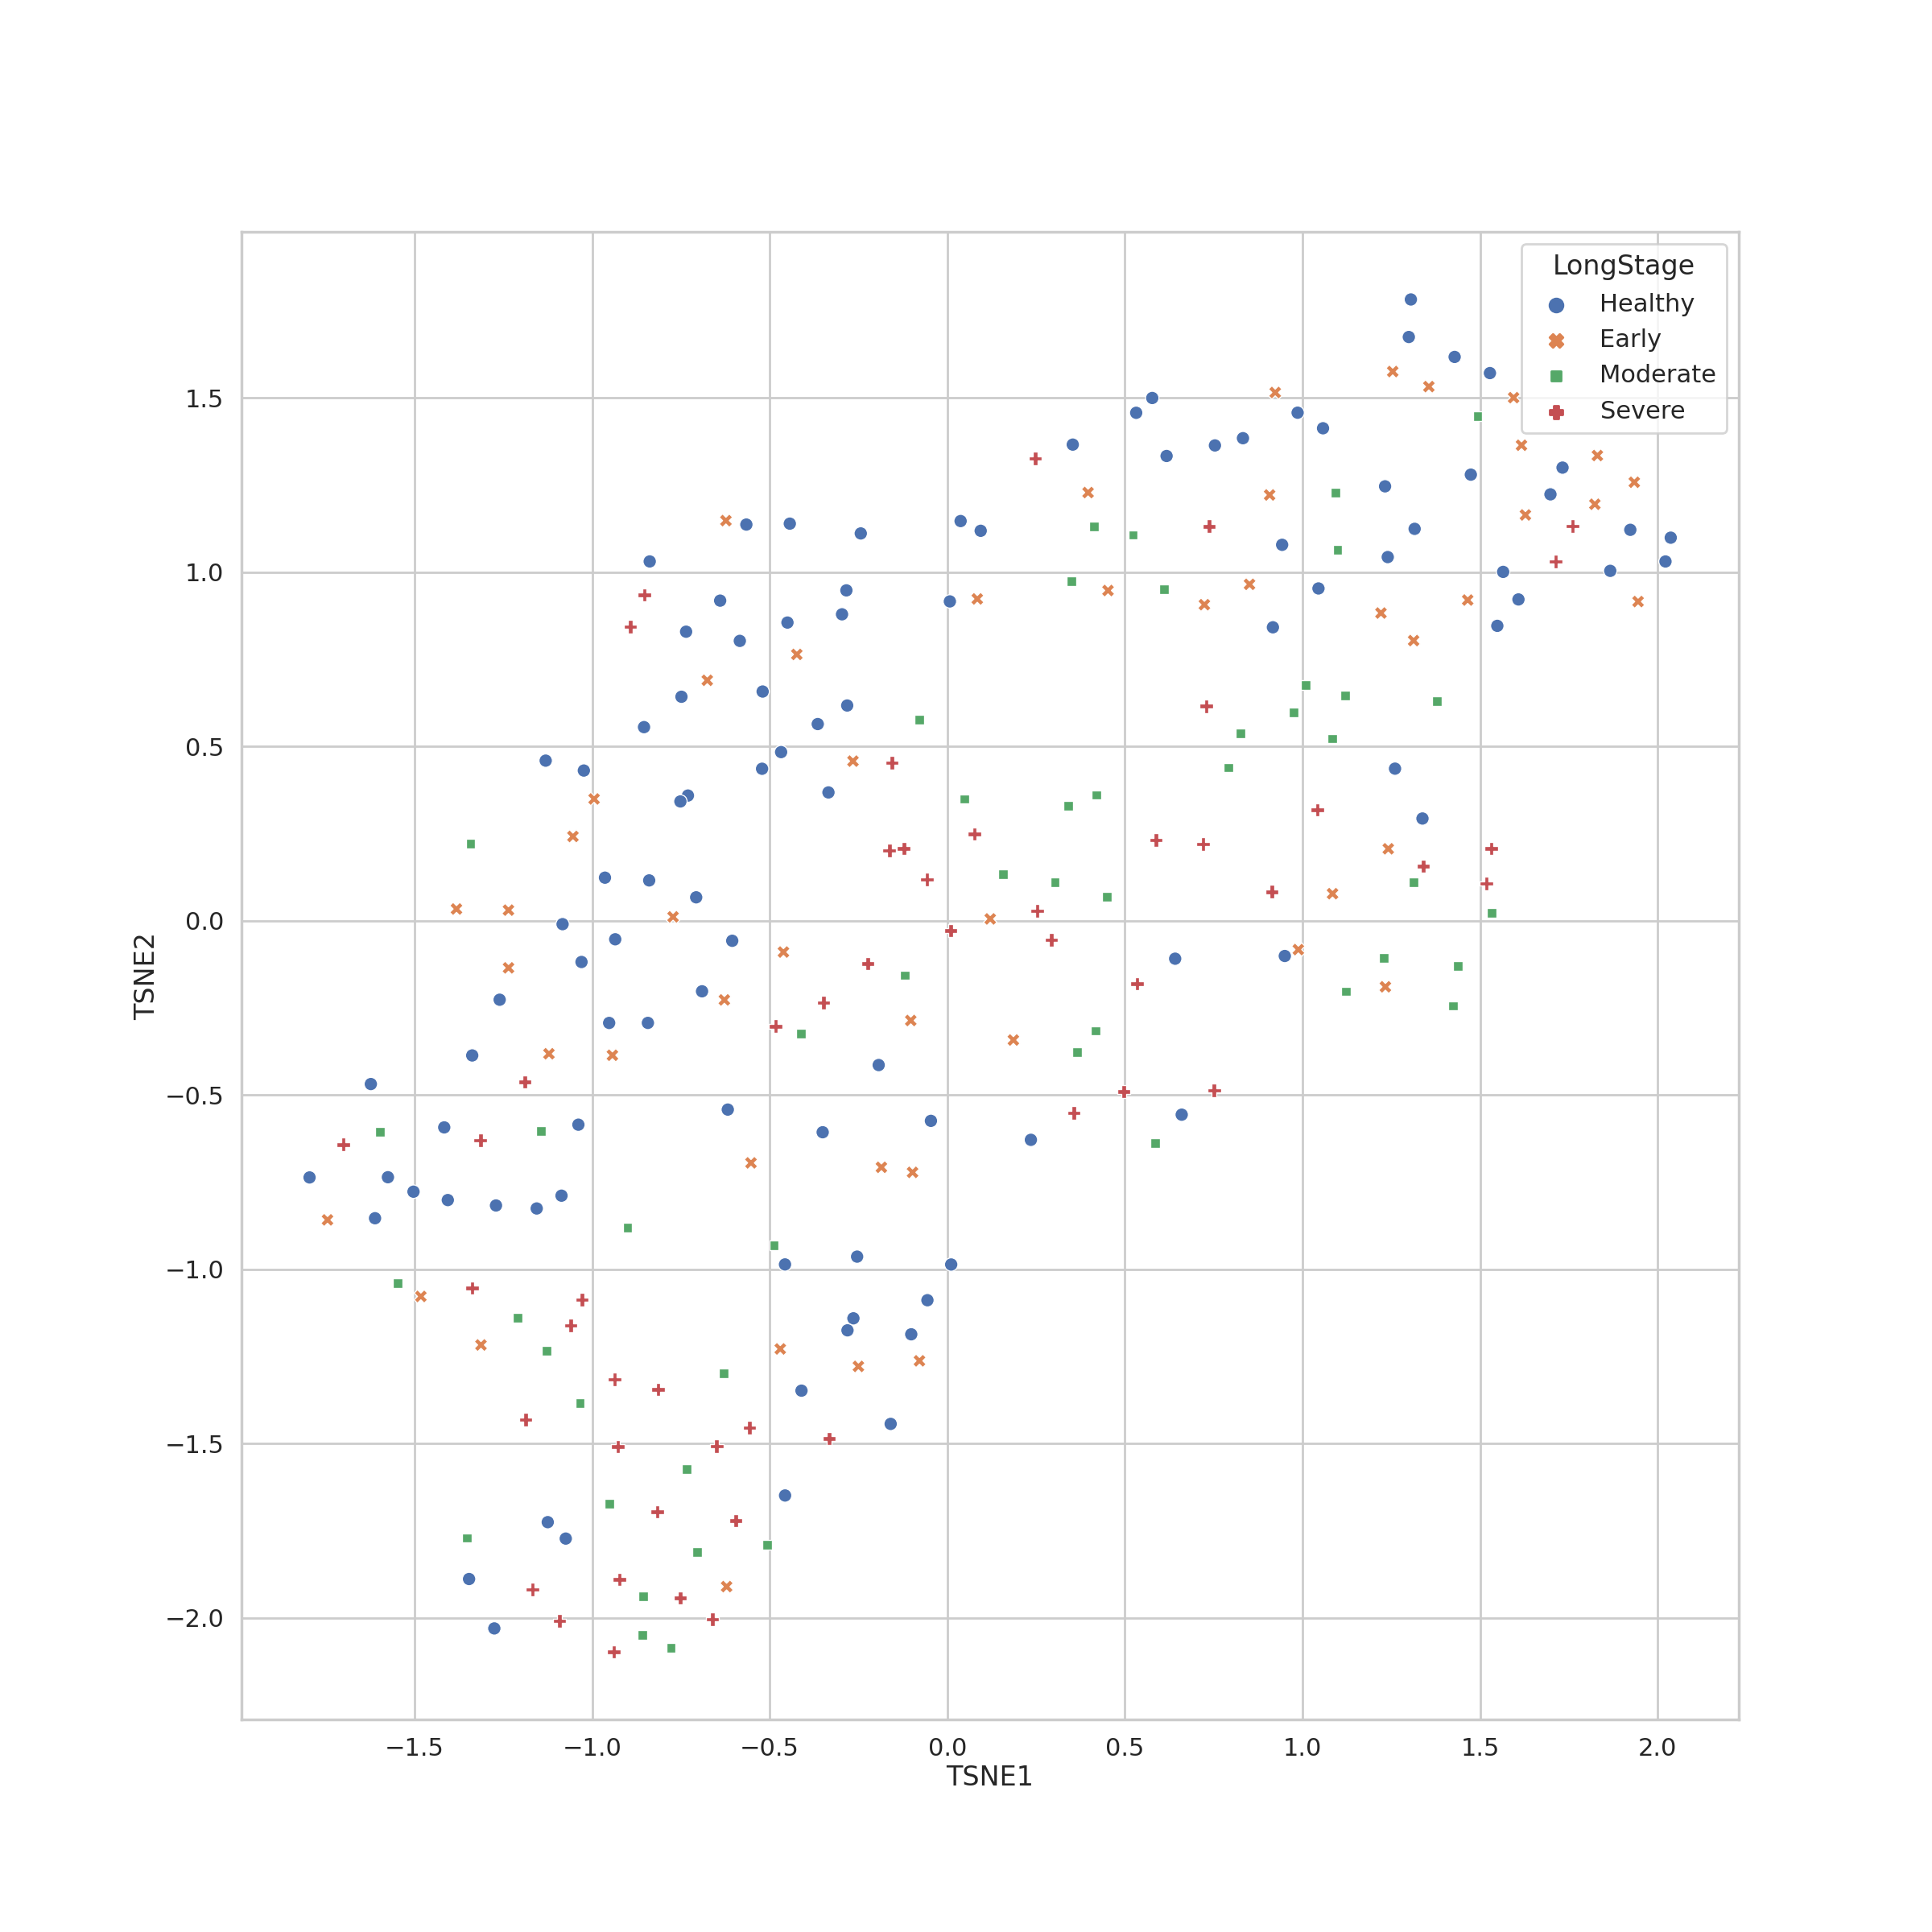
\includegraphics[width=0.6 \linewidth]{figures/BetaDiversity/DADA2.bray_curtis.png}
                \caption{t-SNE Plot from Bray-Curtis Distance Index with DADA2}
                \label{fig:tsne-bray-dada2}
            \end{figure}

            \begin{figure}[p]
                \centering
                $\begin{array}{cc}
                    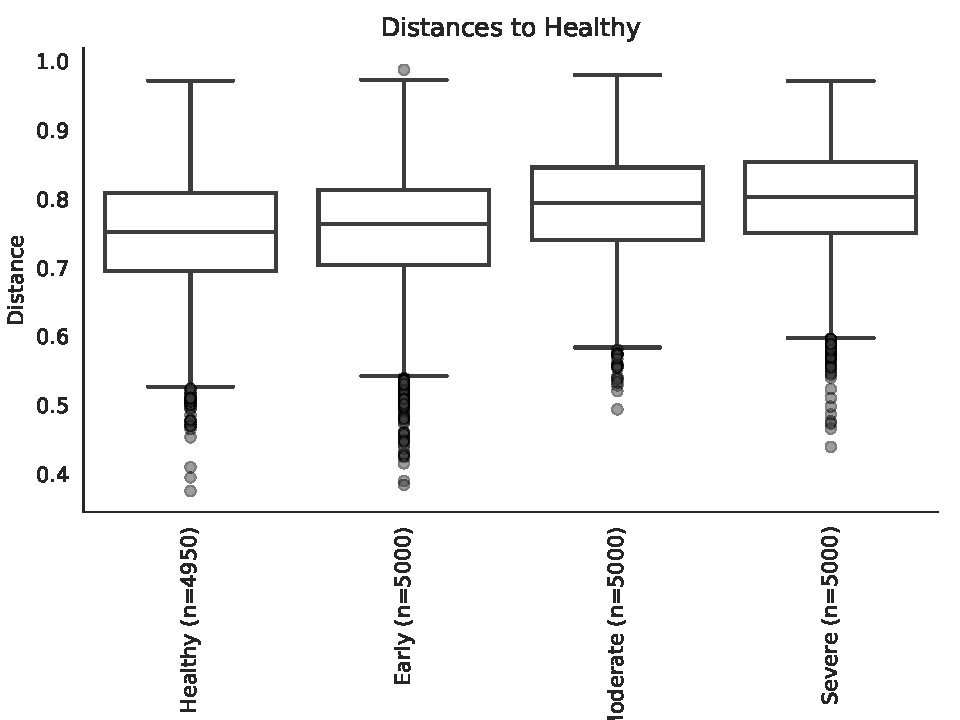
\includegraphics[width=0.4 \linewidth]{figures/BetaDiversity/DADA2/Bray/Healthy.pdf}
                    &
                    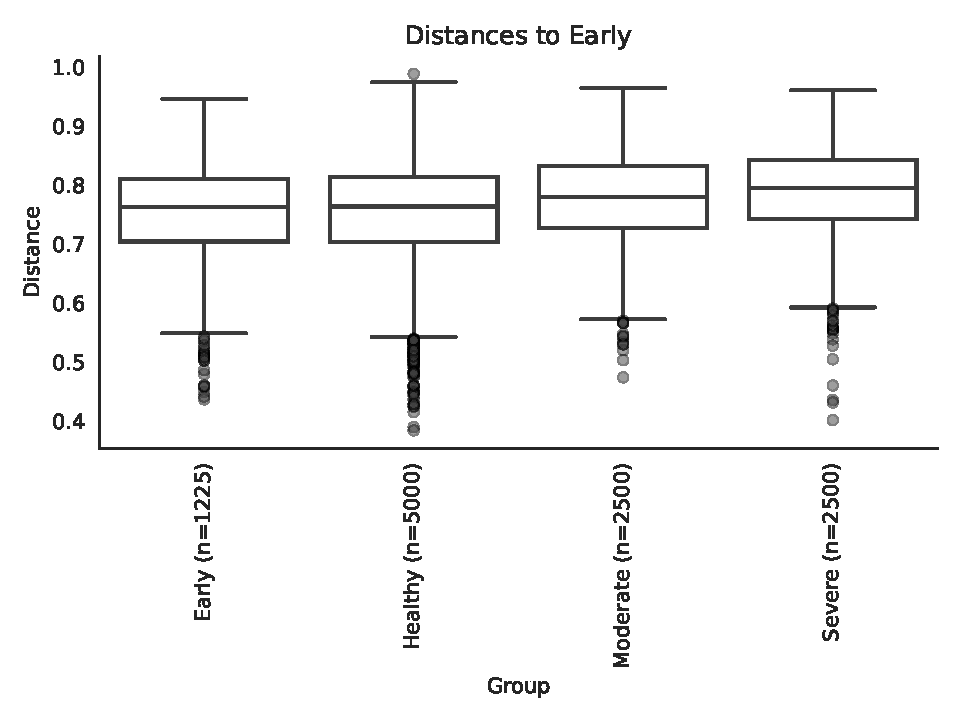
\includegraphics[width=0.4 \linewidth]{figures/BetaDiversity/DADA2/Bray/Early.pdf}
                    \\
                    \mbox{(a) Healthy} & \mbox{(b) Early} \\

                    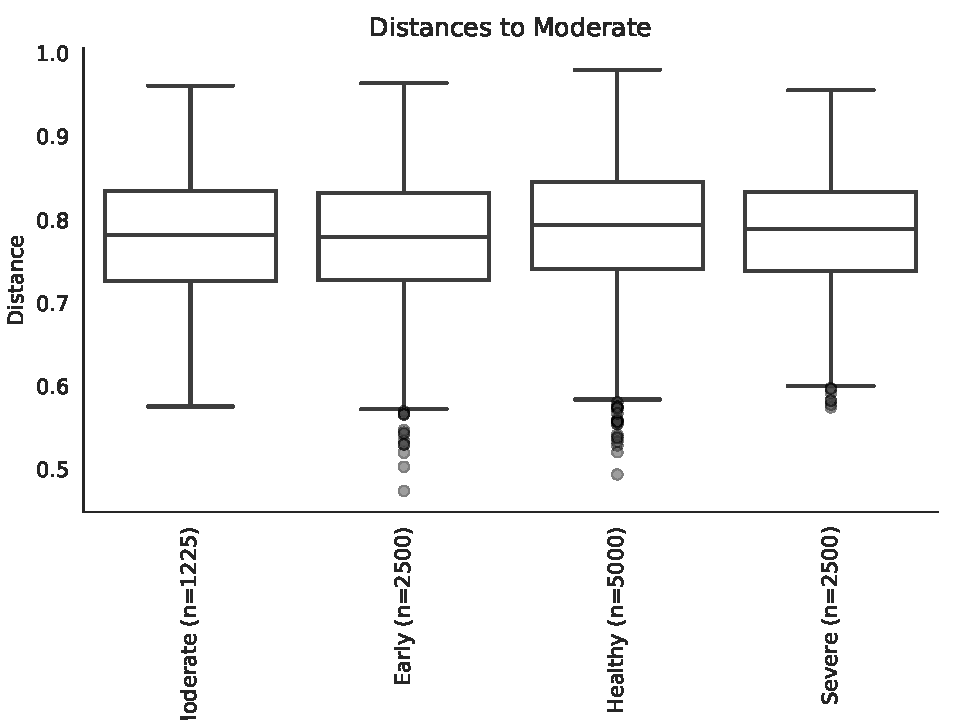
\includegraphics[width=0.4 \linewidth]{figures/BetaDiversity/DADA2/Bray/Moderate.pdf}
                    &
                    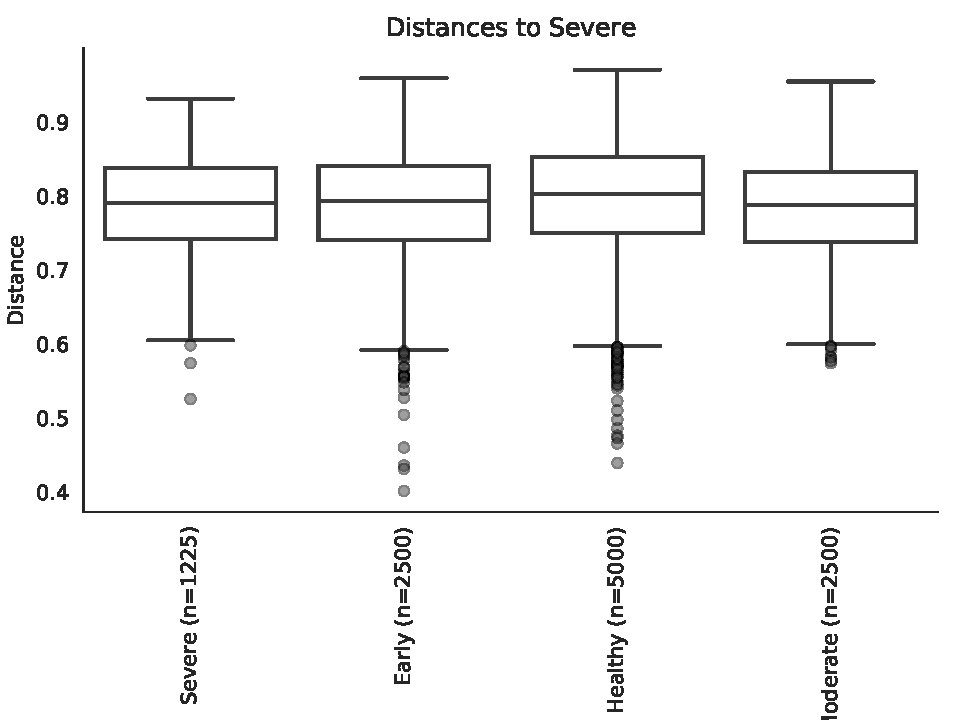
\includegraphics[width=0.4 \linewidth]{figures/BetaDiversity/DADA2/Bray/Severe.pdf}
                    \\
                    \mbox{(c) Moderate} & \mbox{(d) Severe} \\
                \end{array}$
                \caption{Bray-Curtis Distance Index with DADA2}
                \label{fig:bray-dada2}
            \end{figure}

            \begin{figure}[p]
                \centering
                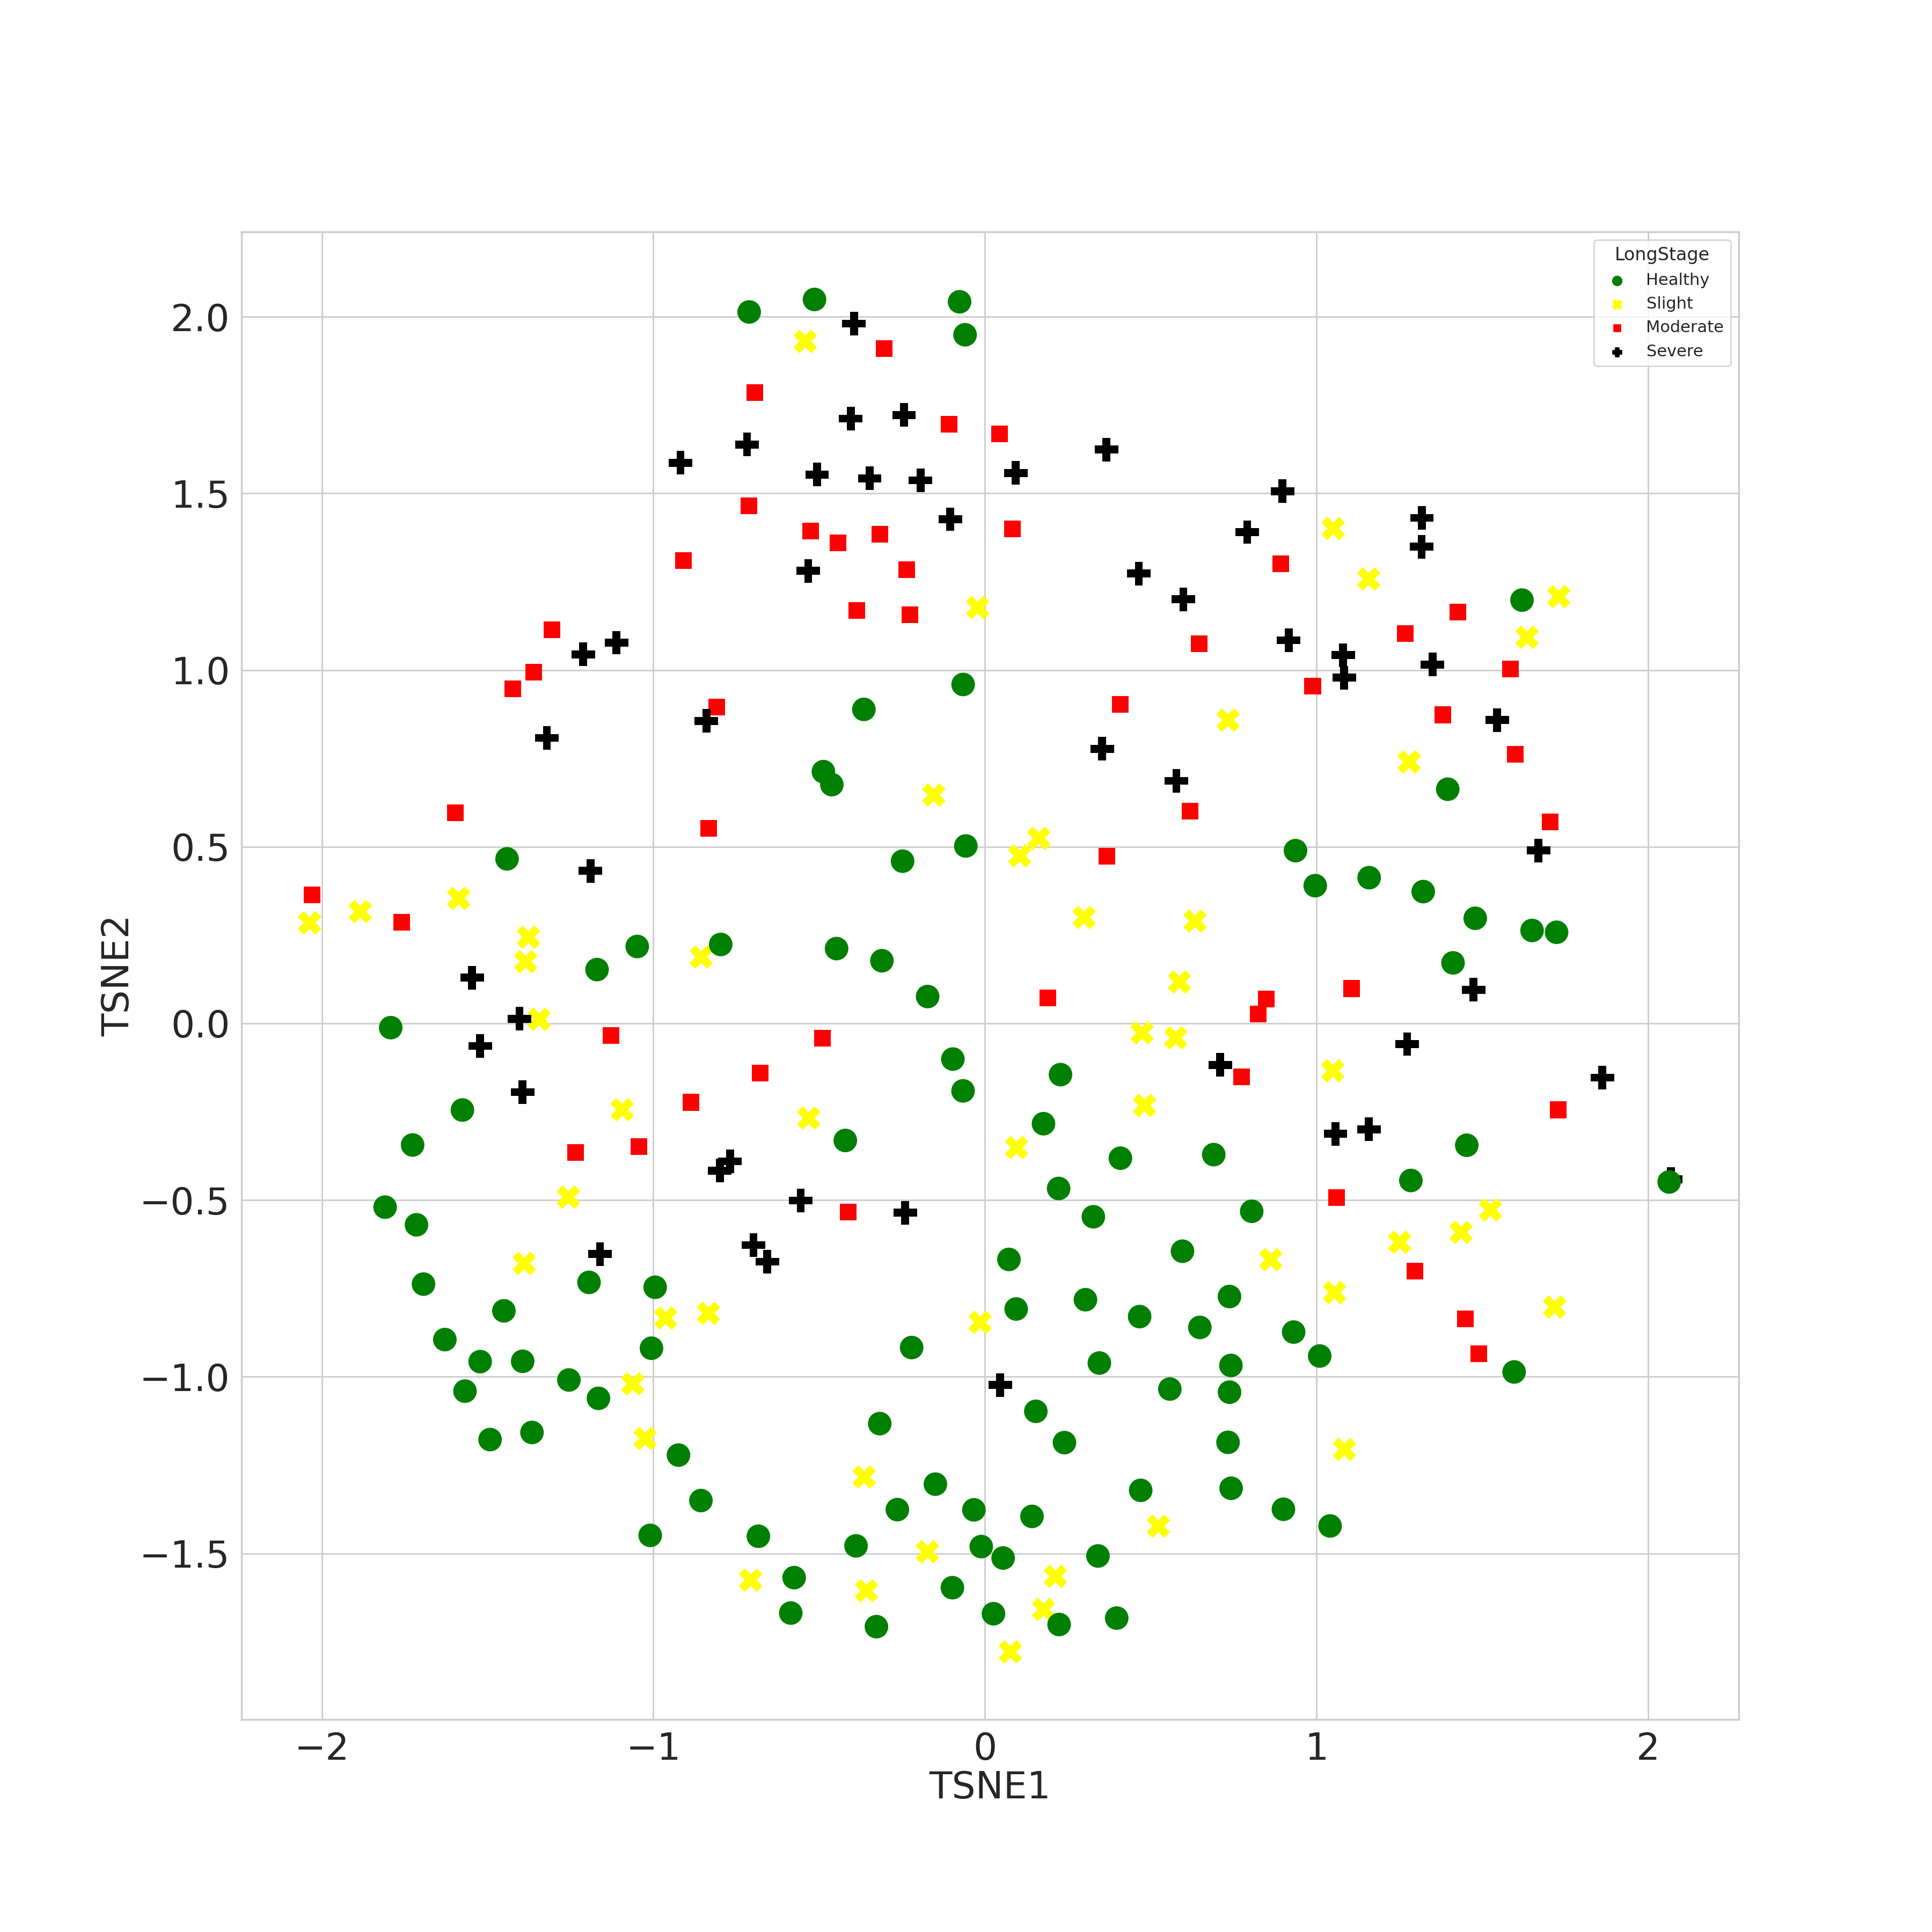
\includegraphics[width=0.6 \linewidth]{figures/BetaDiversity/DADA2.jaccard.png}
                \caption{t-SNE Plot from Jaccard Distance Index with DADA2}
                \label{fig:tsne-jaccard-dada2}
            \end{figure}

            \begin{figure}[p]
                \centering
                $\begin{array}{cc}
                    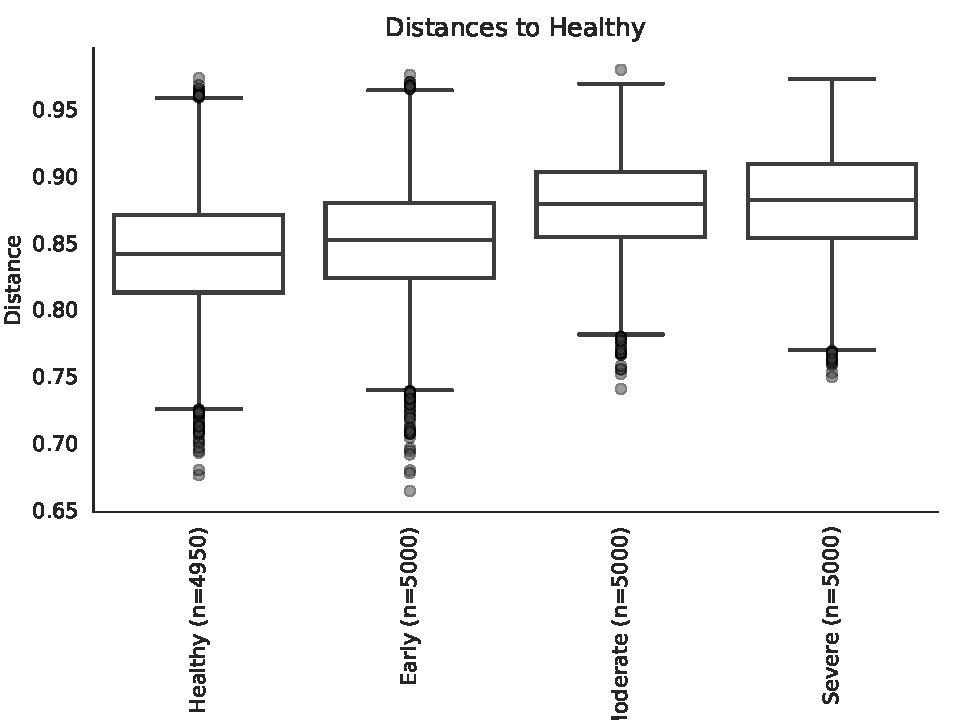
\includegraphics[width=0.4 \linewidth]{figures/BetaDiversity/DADA2/Jaccard/Healthy.pdf}
                    &
                    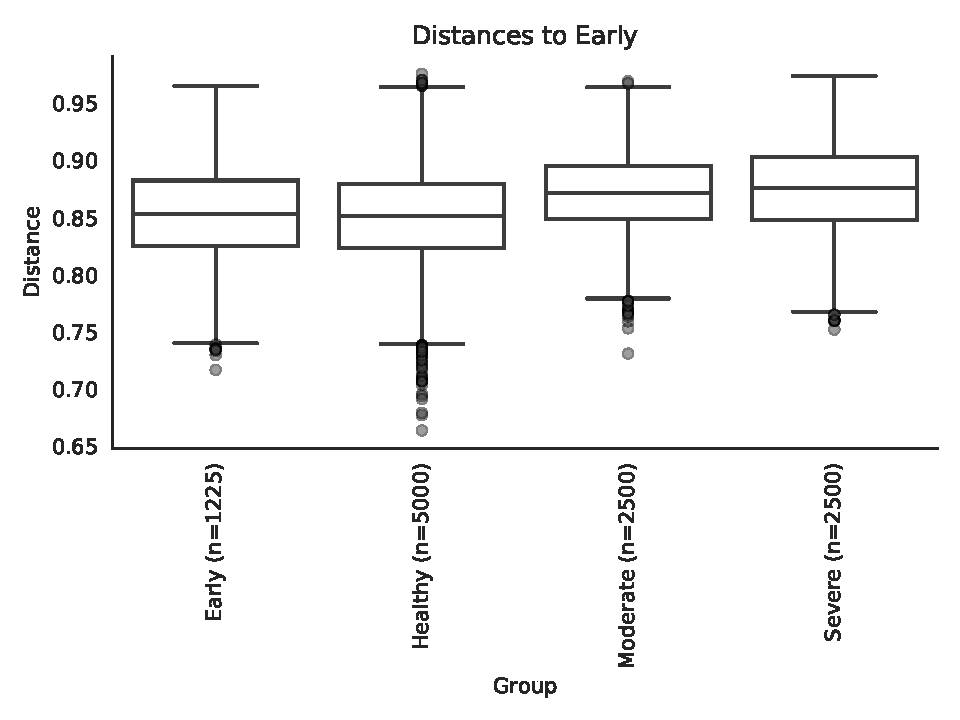
\includegraphics[width=0.4 \linewidth]{figures/BetaDiversity/DADA2/Jaccard/Early.pdf}
                    \\
                    \mbox{(a) Healthy} & \mbox{(b) Early} \\

                    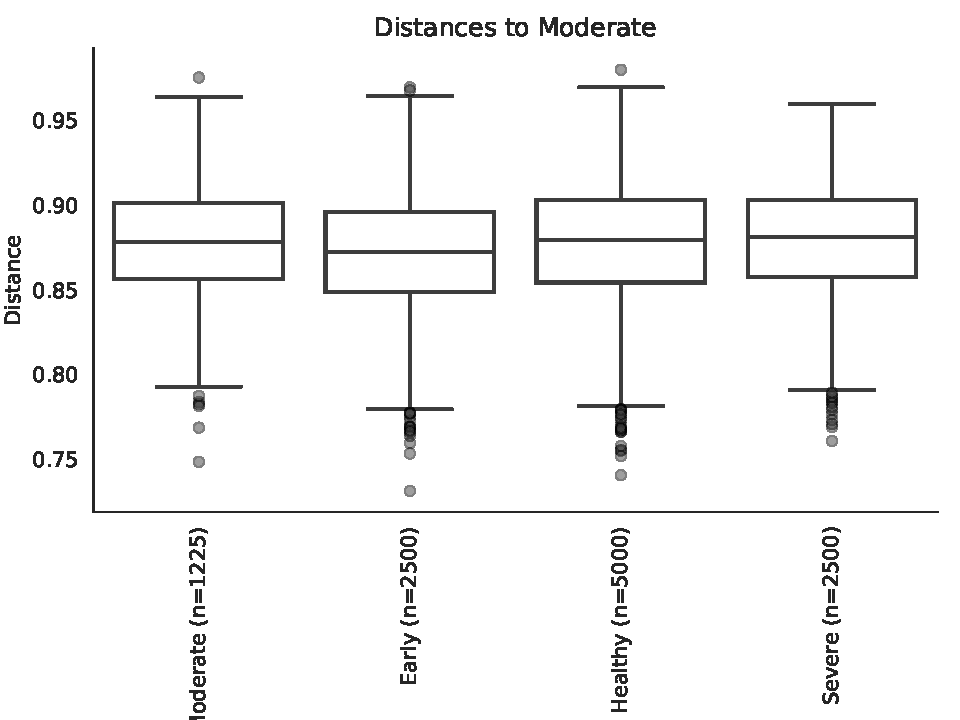
\includegraphics[width=0.4 \linewidth]{figures/BetaDiversity/DADA2/Jaccard/Moderate.pdf}
                    &
                    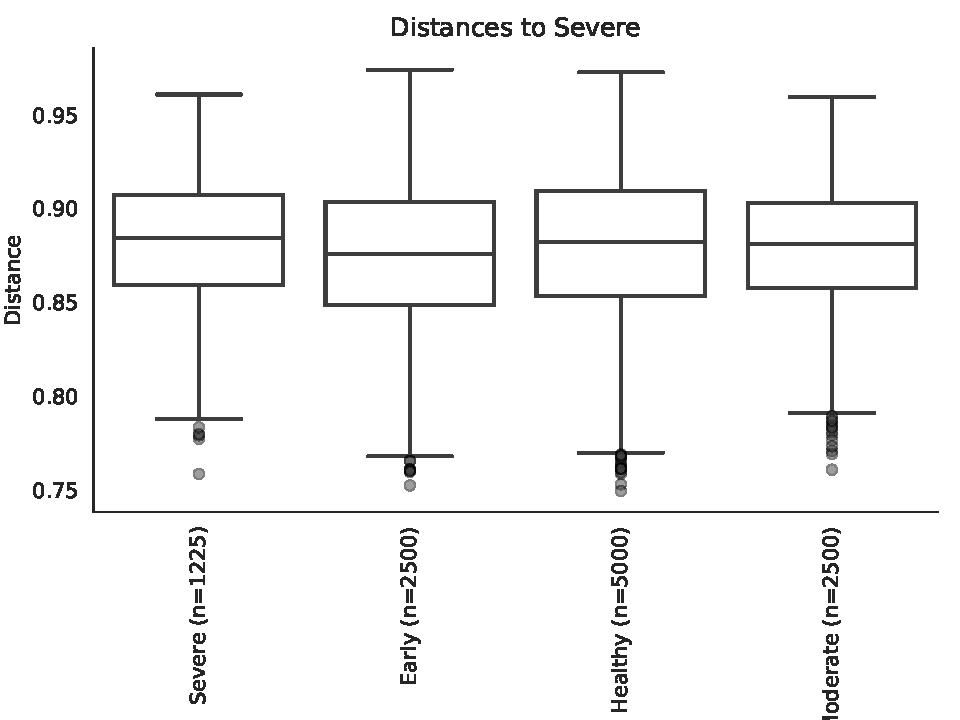
\includegraphics[width=0.4 \linewidth]{figures/BetaDiversity/DADA2/Jaccard/Severe.pdf}
                    \\
                    \mbox{(c) Moderate} & \mbox{(d) Severe} \\
                \end{array}$
                \caption{Jaccard Distance Index with DADA2}
                \label{fig:jaccard-dada2}
            \end{figure}

            \begin{figure}[p]
                \centering
                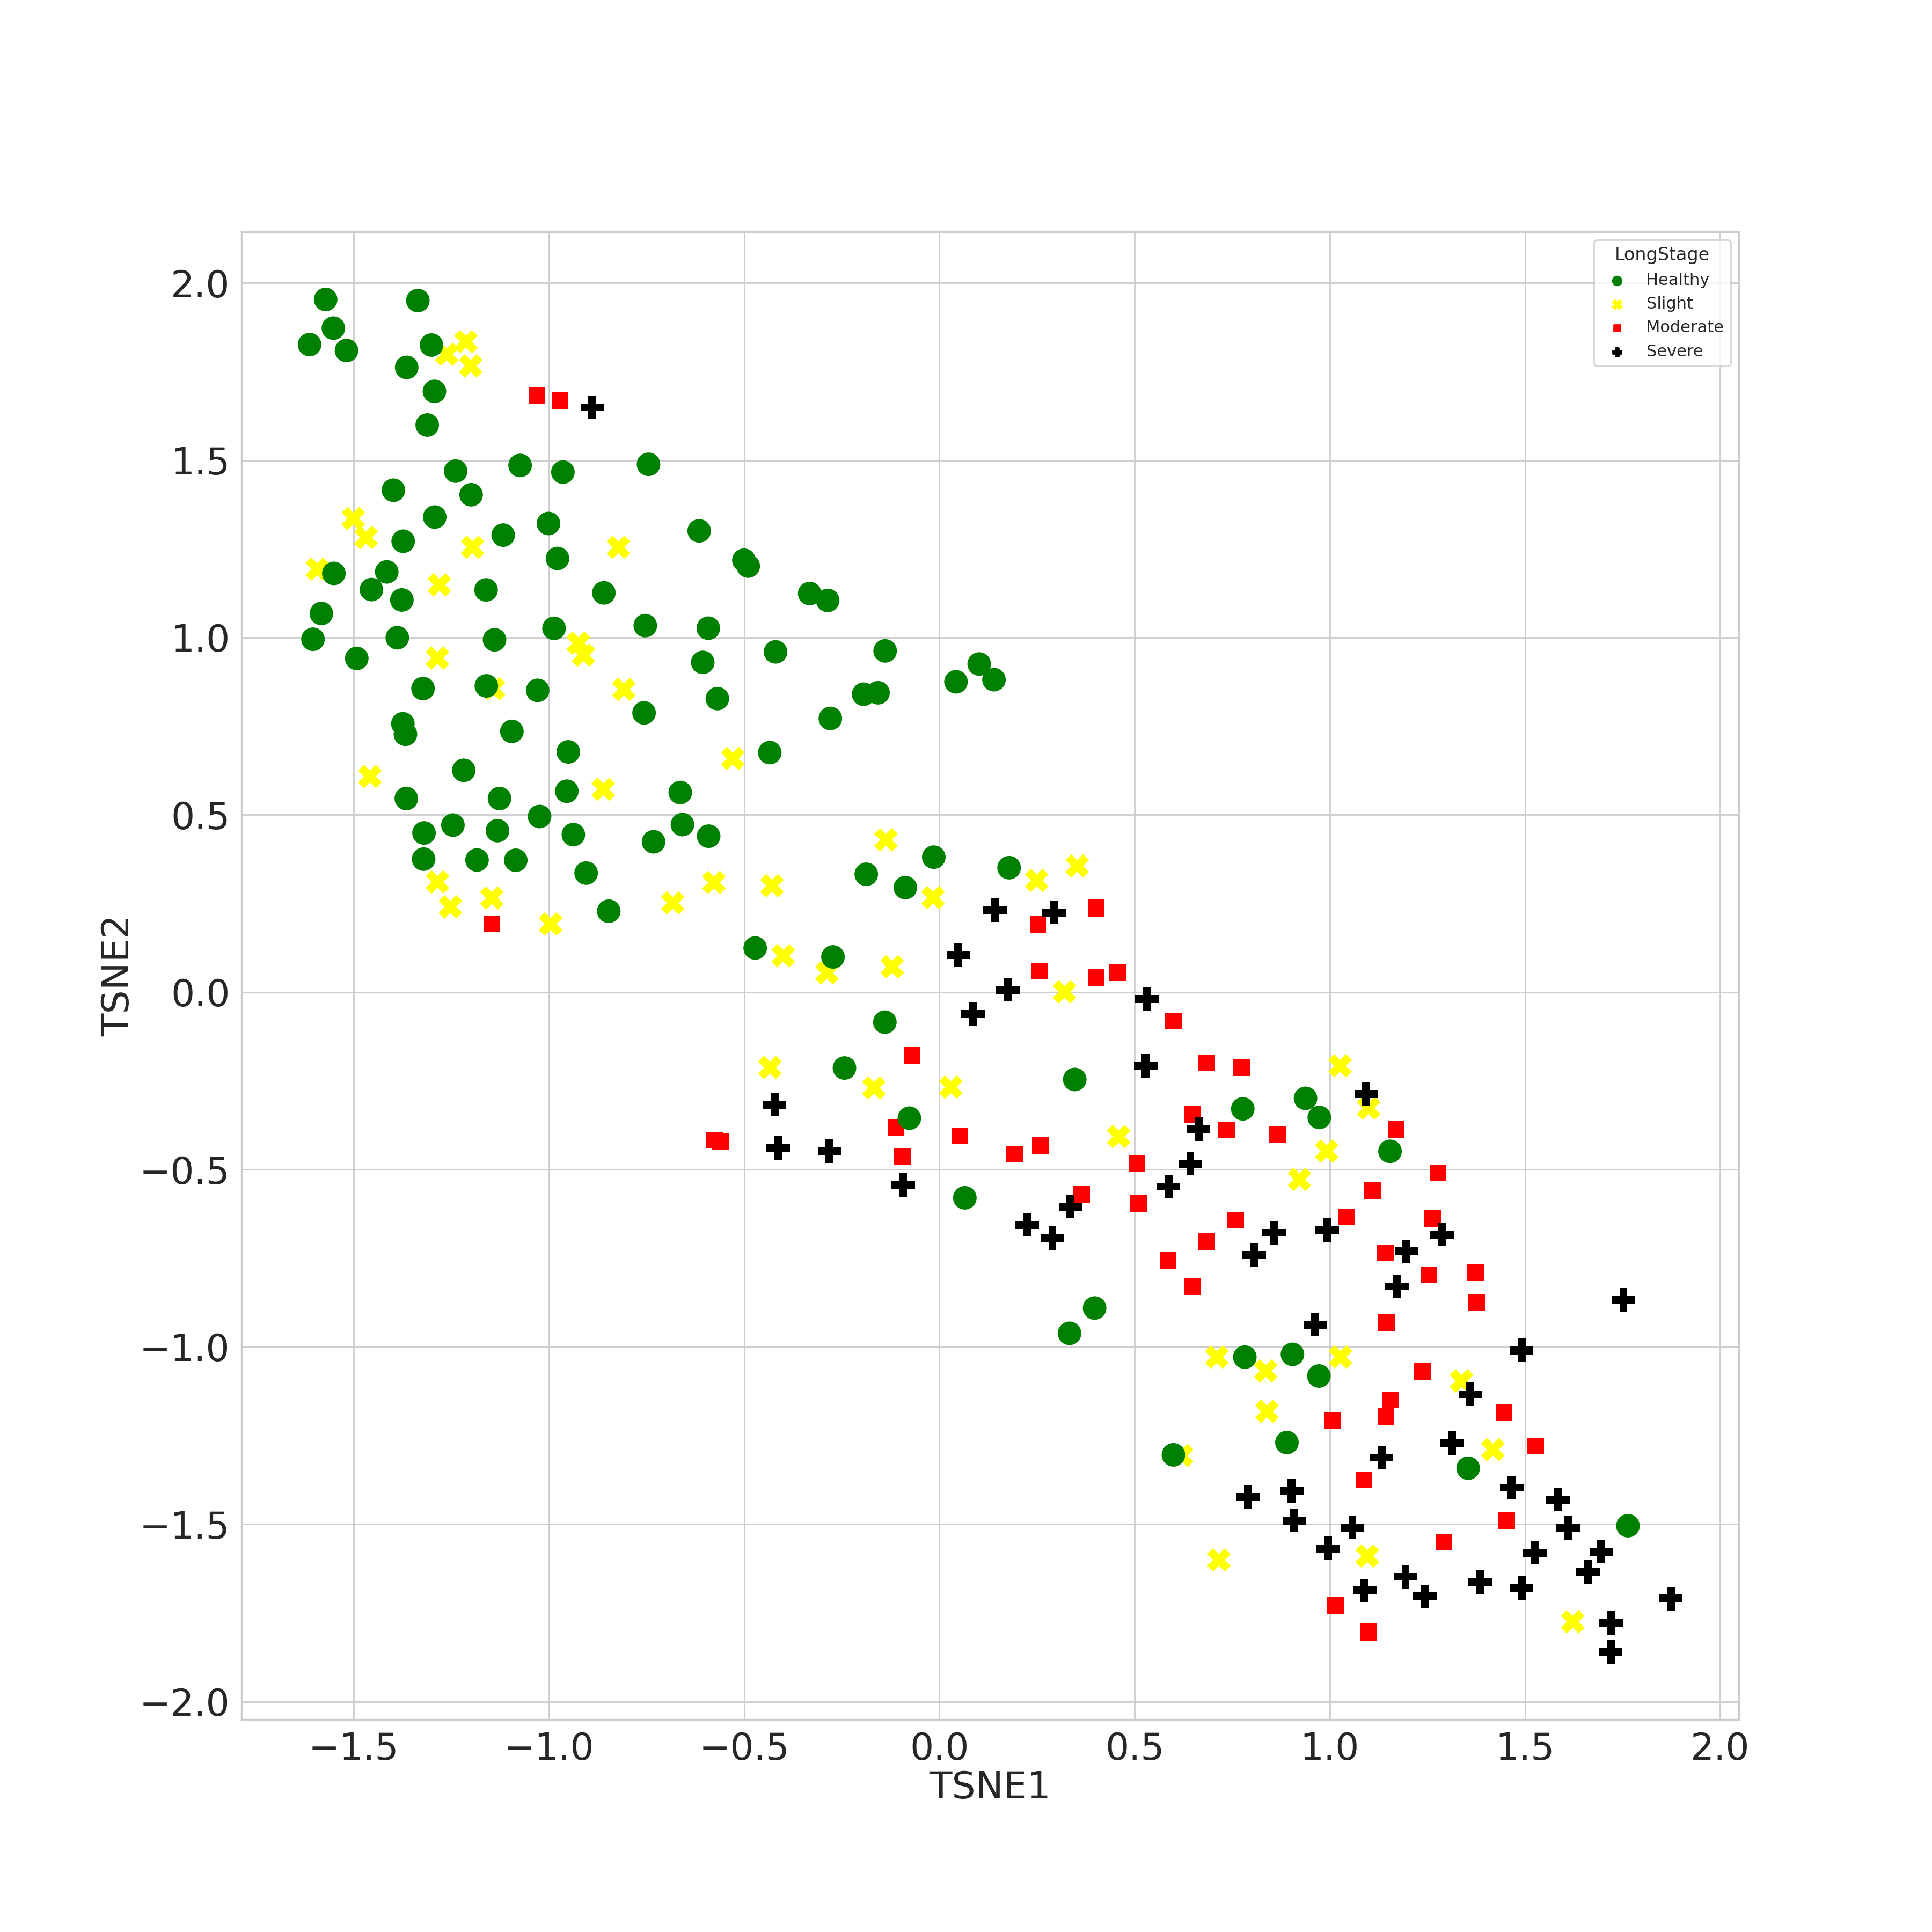
\includegraphics[width=0.6 \linewidth]{figures/BetaDiversity/DADA2.unweighted_unifrac.png}
                \caption{t-SNE Plot from Unweighted UniFrac Distance Index with DADA2}
                \label{fig:tsne-unweighted-dada2}
            \end{figure}

            \begin{figure}[p]
                \centering
                $\begin{array}{cc}
                    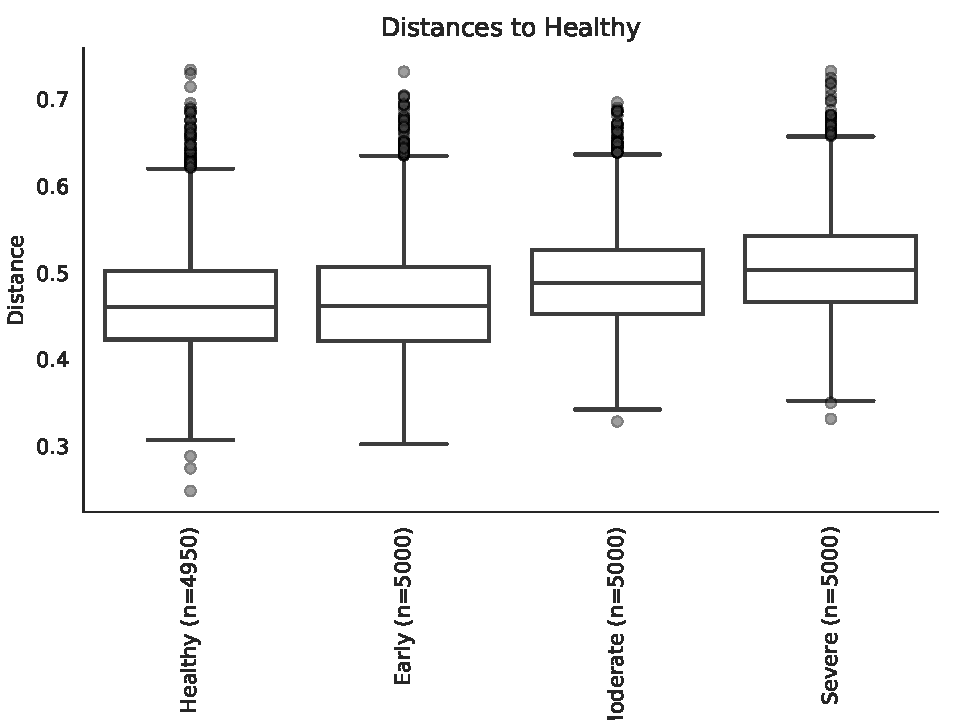
\includegraphics[width=0.4 \linewidth]{figures/BetaDiversity/DADA2/UnweightedUnifrac/Healthy.pdf}
                    &
                    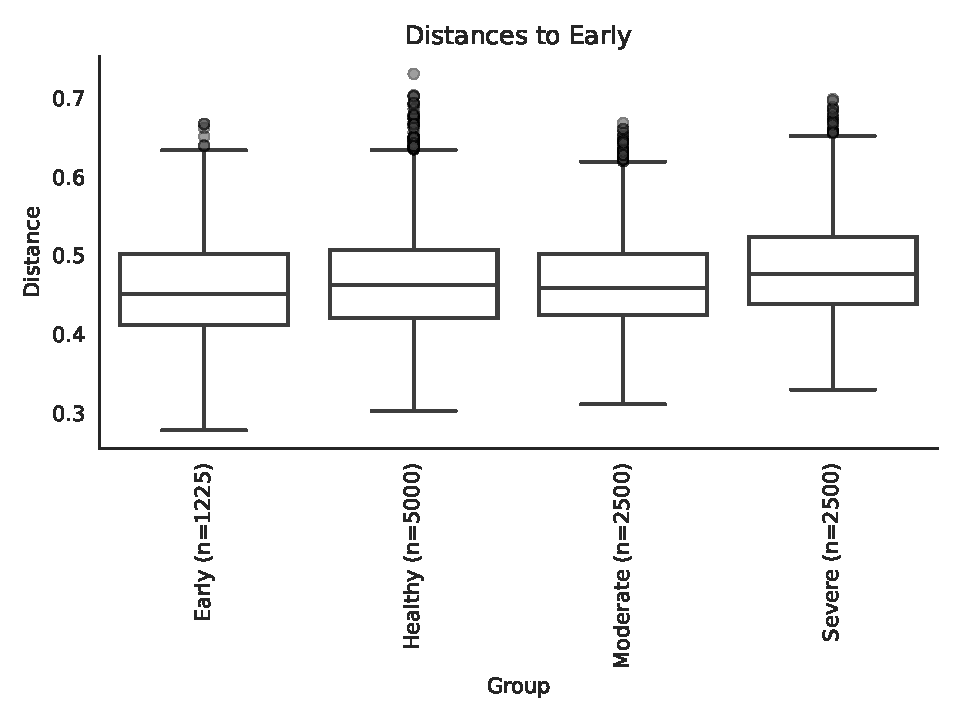
\includegraphics[width=0.4 \linewidth]{figures/BetaDiversity/DADA2/UnweightedUnifrac/Early.pdf}
                    \\
                    \mbox{(a) Healthy} & \mbox{(b) Early} \\

                    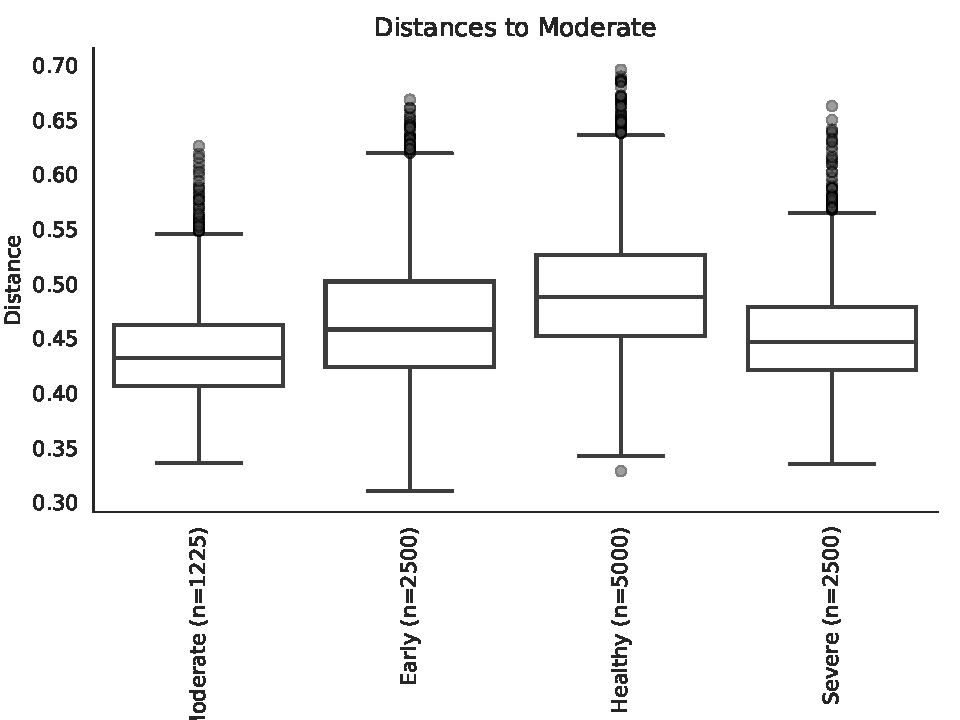
\includegraphics[width=0.4 \linewidth]{figures/BetaDiversity/DADA2/UnweightedUnifrac/Moderate.pdf}
                    &
                    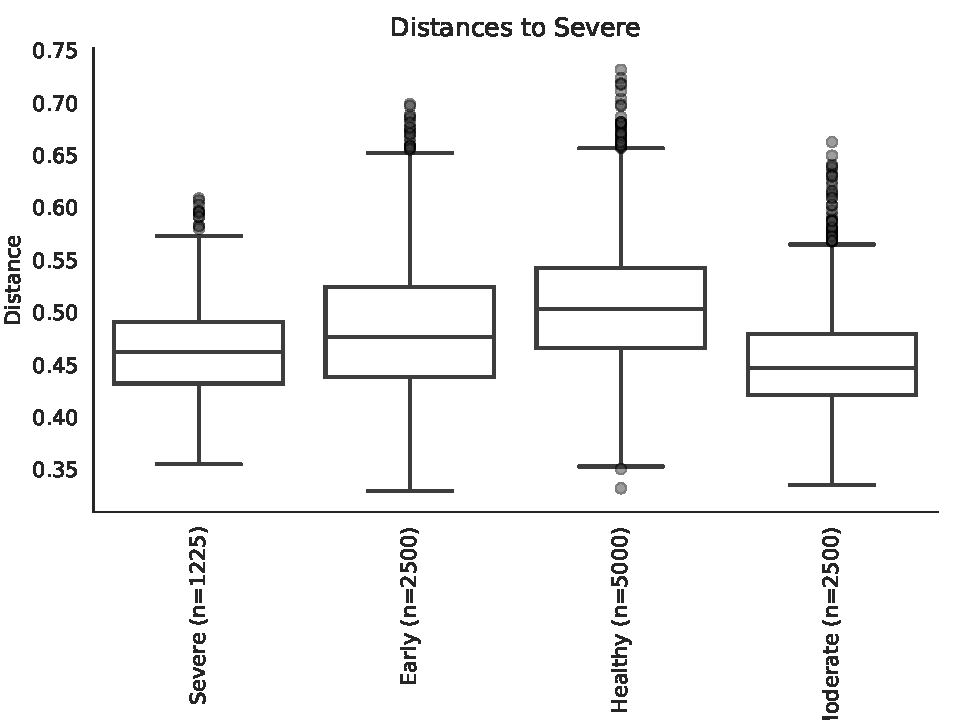
\includegraphics[width=0.4 \linewidth]{figures/BetaDiversity/DADA2/UnweightedUnifrac/Severe.pdf}
                    \\
                    \mbox{(c) Moderate} & \mbox{(d) Severe} \\
                \end{array}$
                \caption{Unweighted UniFrac Distance Index with DADA2}
                \label{fig:unweighted-dada2}
            \end{figure}

            \begin{figure}[p]
                \centering
                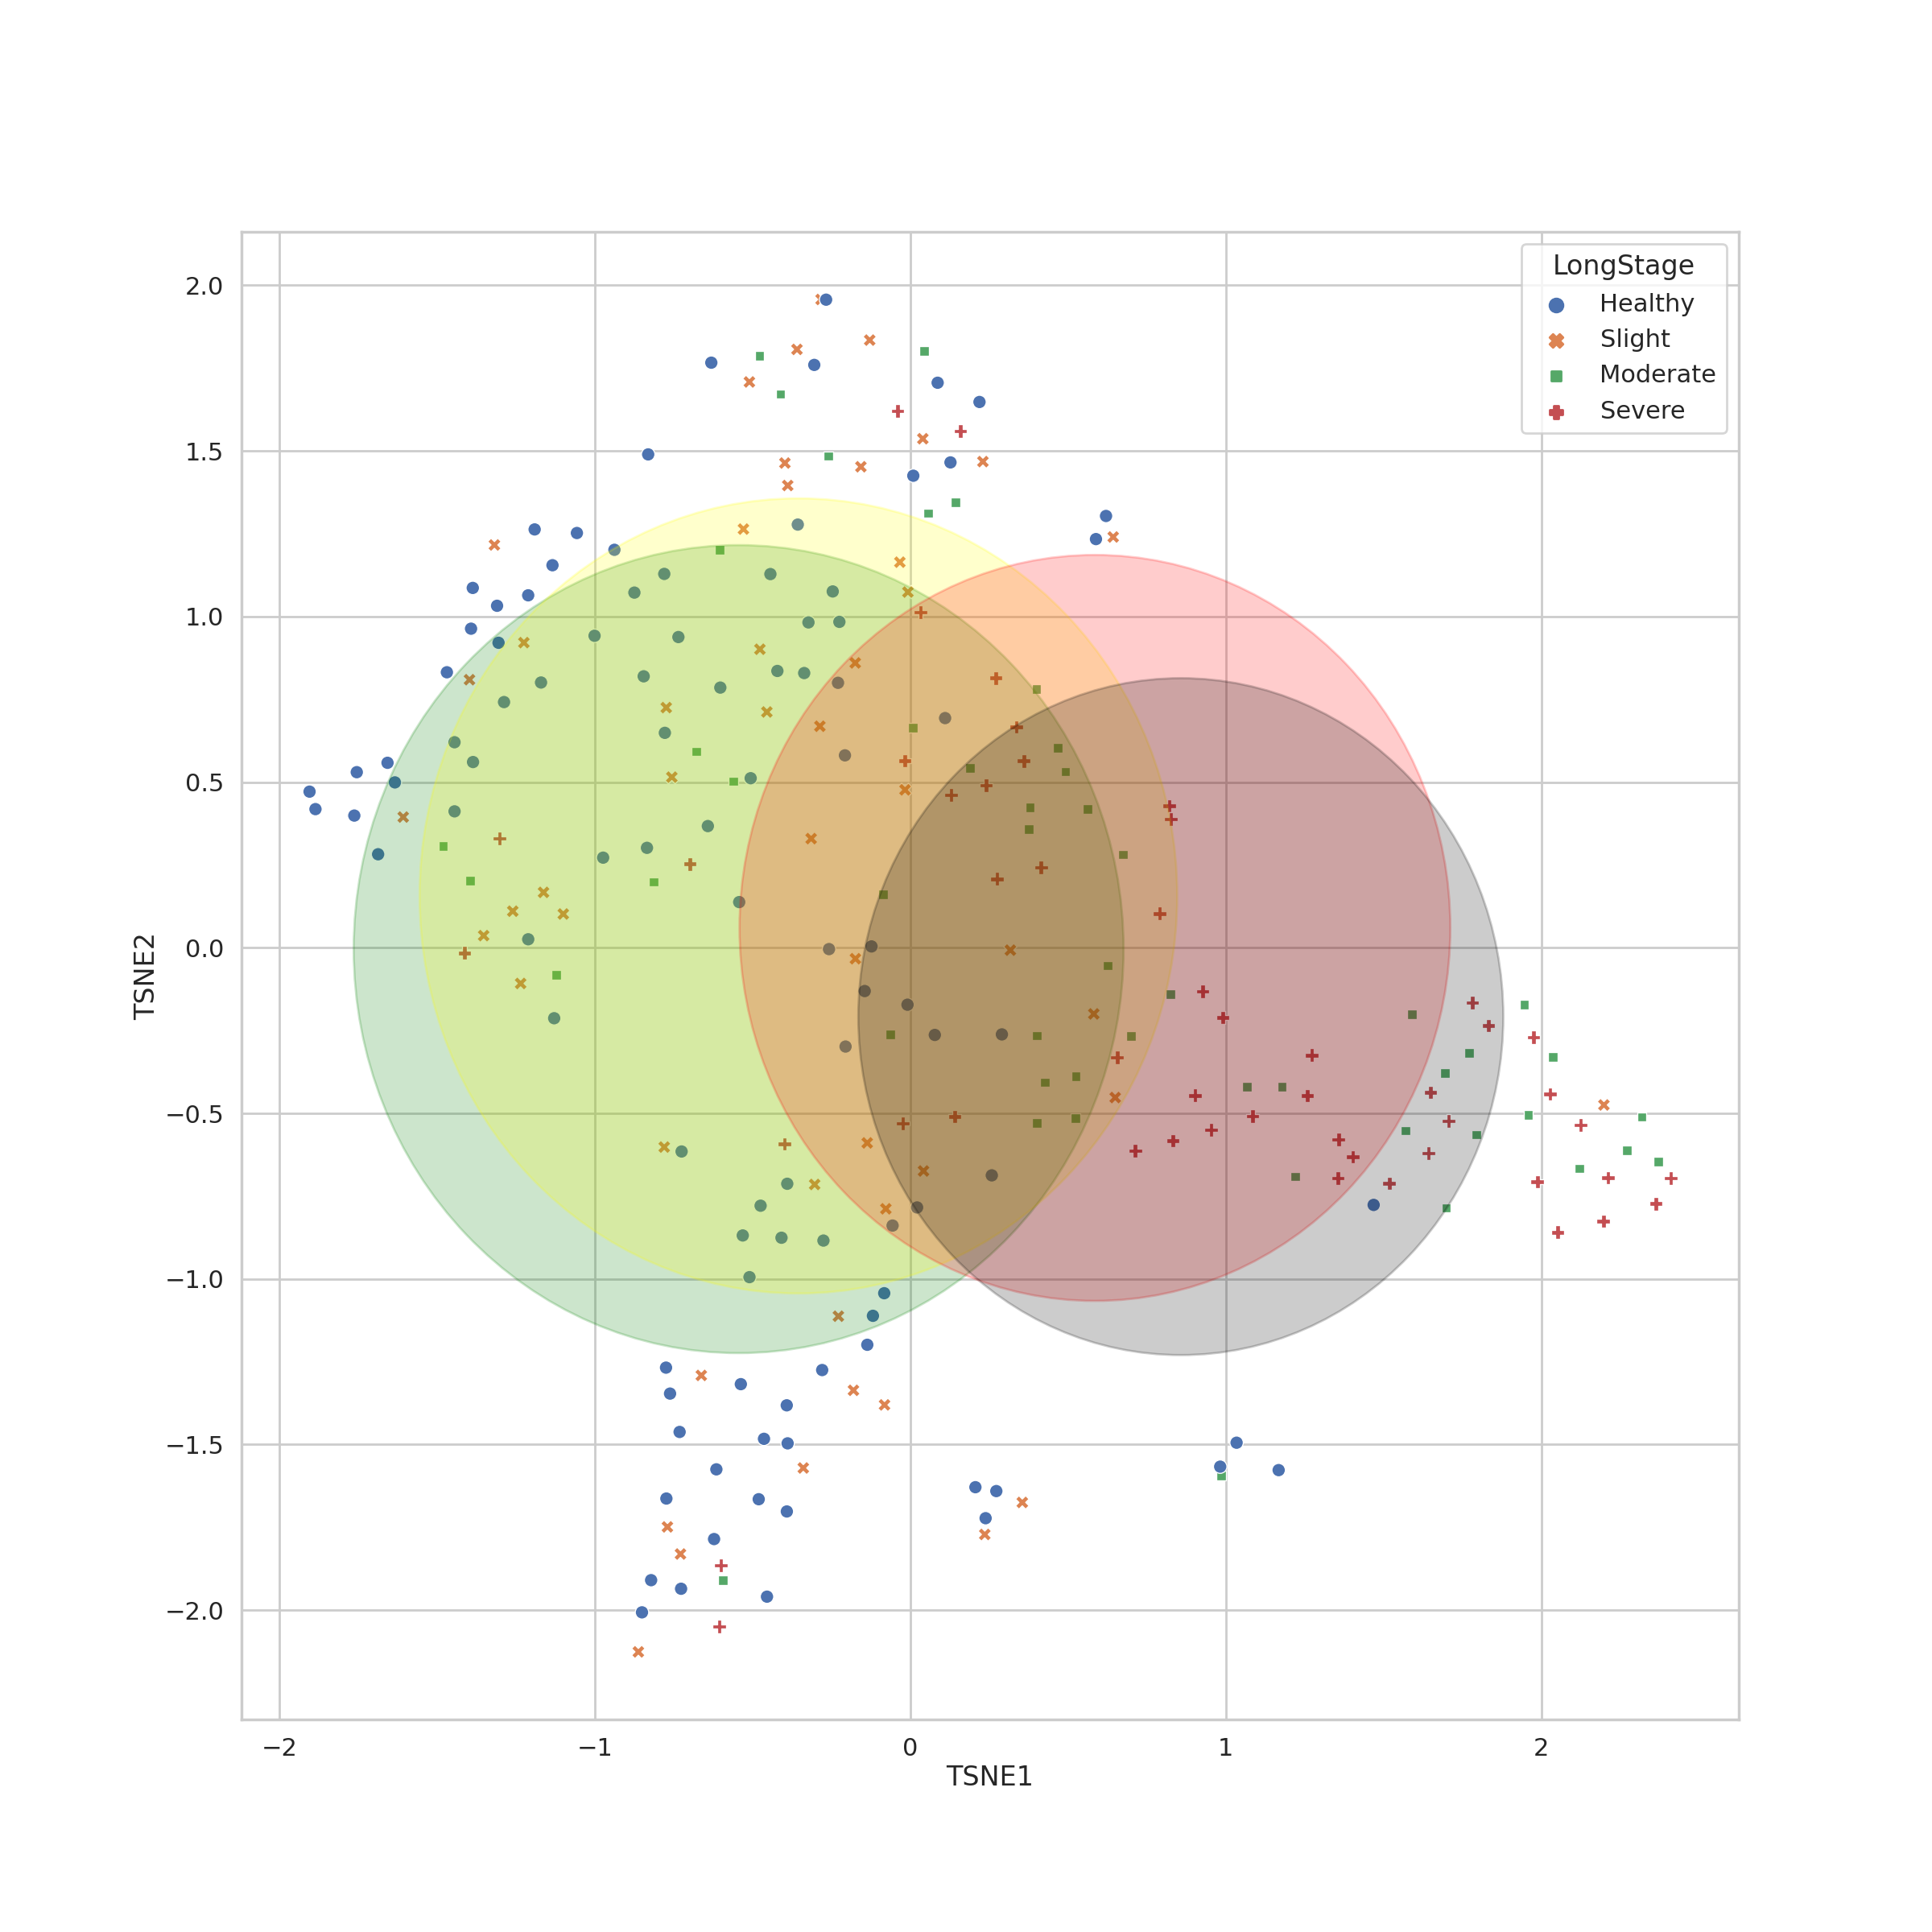
\includegraphics[width=0.6 \linewidth]{figures/BetaDiversity/DADA2.weighted_unifrac.png}
                \caption{t-SNE Plot from Weighted UniFrac Distance Index with DADA2}
                \label{fig:tsne-weighted-dada2}
            \end{figure}

            \begin{figure}[p]
                \centering
                $\begin{array}{cc}
                    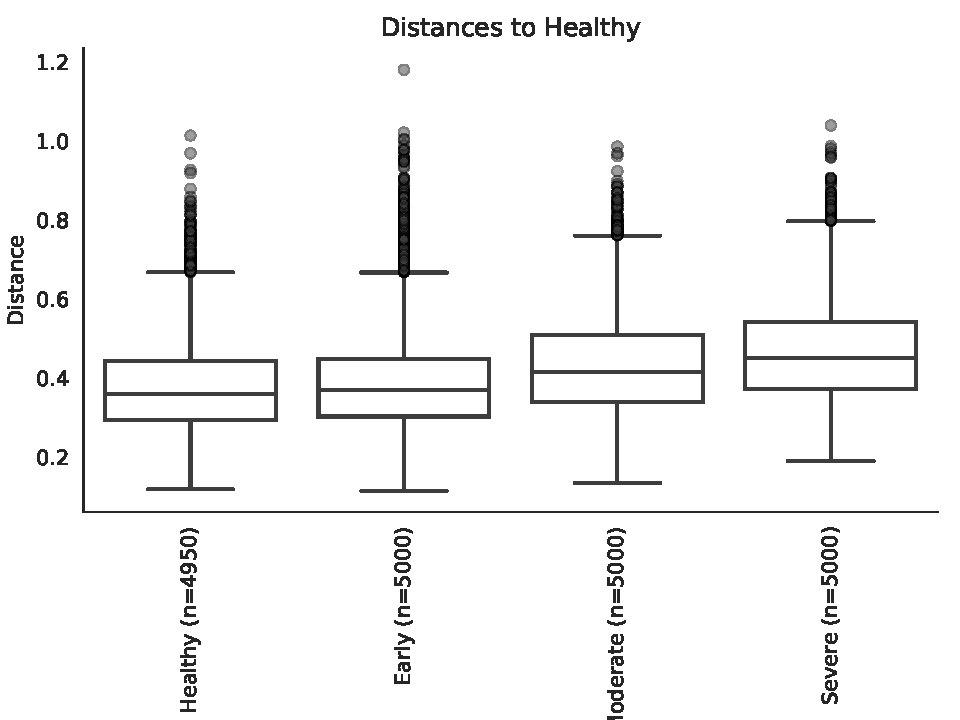
\includegraphics[width=0.4 \linewidth]{figures/BetaDiversity/DADA2/WeightedUnifrac/Healthy.pdf}
                    &
                    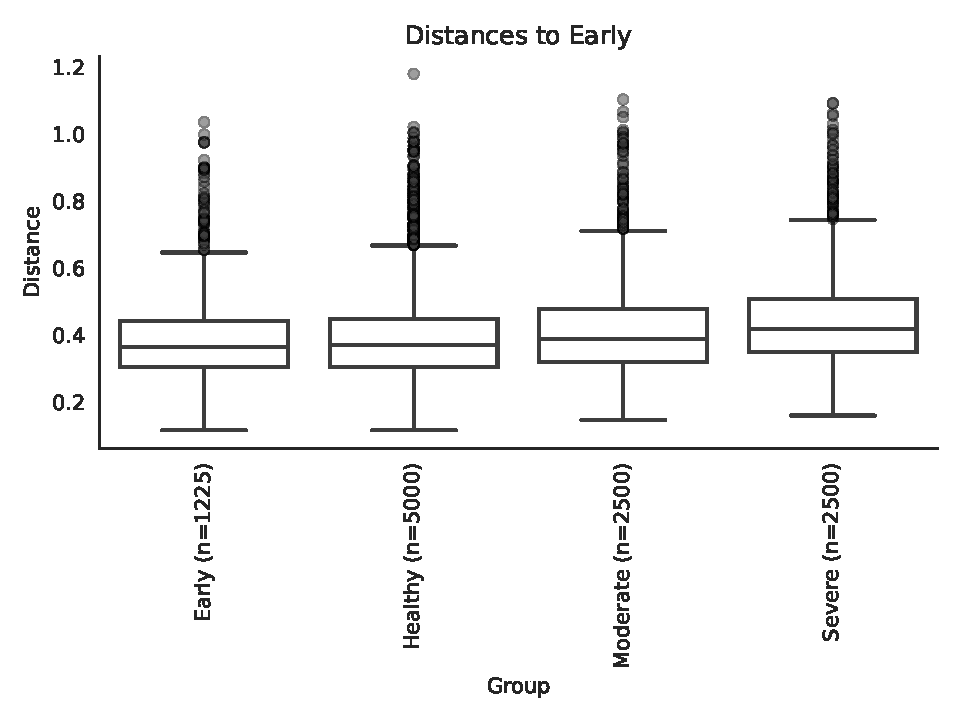
\includegraphics[width=0.4 \linewidth]{figures/BetaDiversity/DADA2/WeightedUnifrac/Early.pdf}
                    \\
                    \mbox{(a) Healthy} & \mbox{(b) Early} \\

                    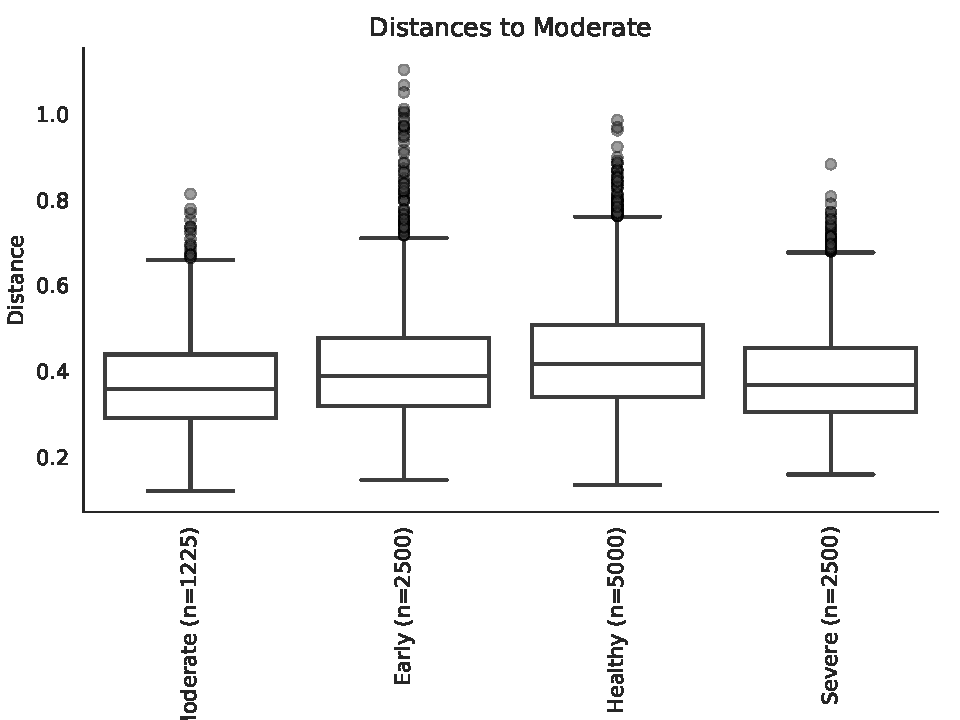
\includegraphics[width=0.4 \linewidth]{figures/BetaDiversity/DADA2/WeightedUnifrac/Moderate.pdf}
                    &
                    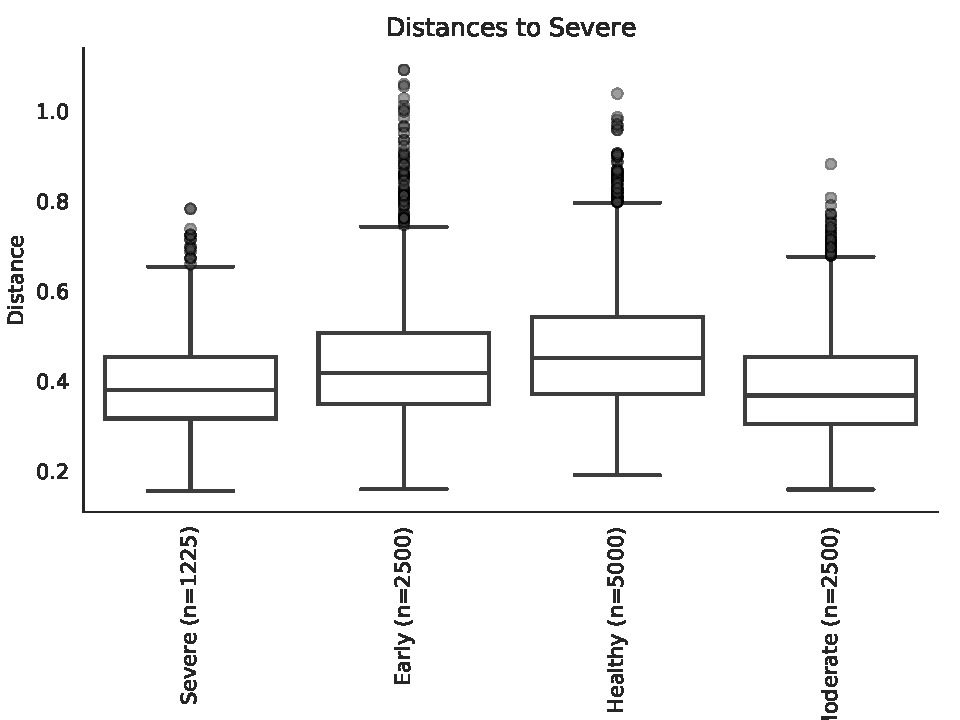
\includegraphics[width=0.4 \linewidth]{figures/BetaDiversity/DADA2/WeightedUnifrac/Severe.pdf}
                    \\
                    \mbox{(c) Moderate} & \mbox{(d) Severe} \\
                \end{array}$
                \caption{Weighted UniFrac Distance Index with DADA2}
                \label{fig:weighted-dada2}
            \end{figure}

            \begin{table}[p]
                \centering
                \caption{Bray-Curtis Distance Index with Deblur}
                \label{tb:bray-deblur}
                \csvautobooktabular{csv/BetaDiversity/Deblur/Bray.csv}
            \end{table}

            \begin{table}[p]
                \centering
                \caption{Jaccard Distance Index with Deblur}
                \label{tb:jaccard-deblur}
                \csvautobooktabular{csv/BetaDiversity/Deblur/Jaccard.csv}
            \end{table}

            \begin{table}[p]
                \centering
                \caption{Unweighted UniFrac Distance Index with Deblur}
                \label{tb:unweighted-deblur}
                \csvautobooktabular{csv/BetaDiversity/Deblur/UnweightedUniFrac.csv}
            \end{table}

            \begin{table}[p]
                \centering
                \caption{Weighted UniFrac Distance Index with Deblur}
                \label{tb:weighted-deblur}
                \csvautobooktabular{csv/BetaDiversity/Deblur/WeightedUniFrac.csv}
            \end{table}

            \begin{figure}[p]
                \centering
                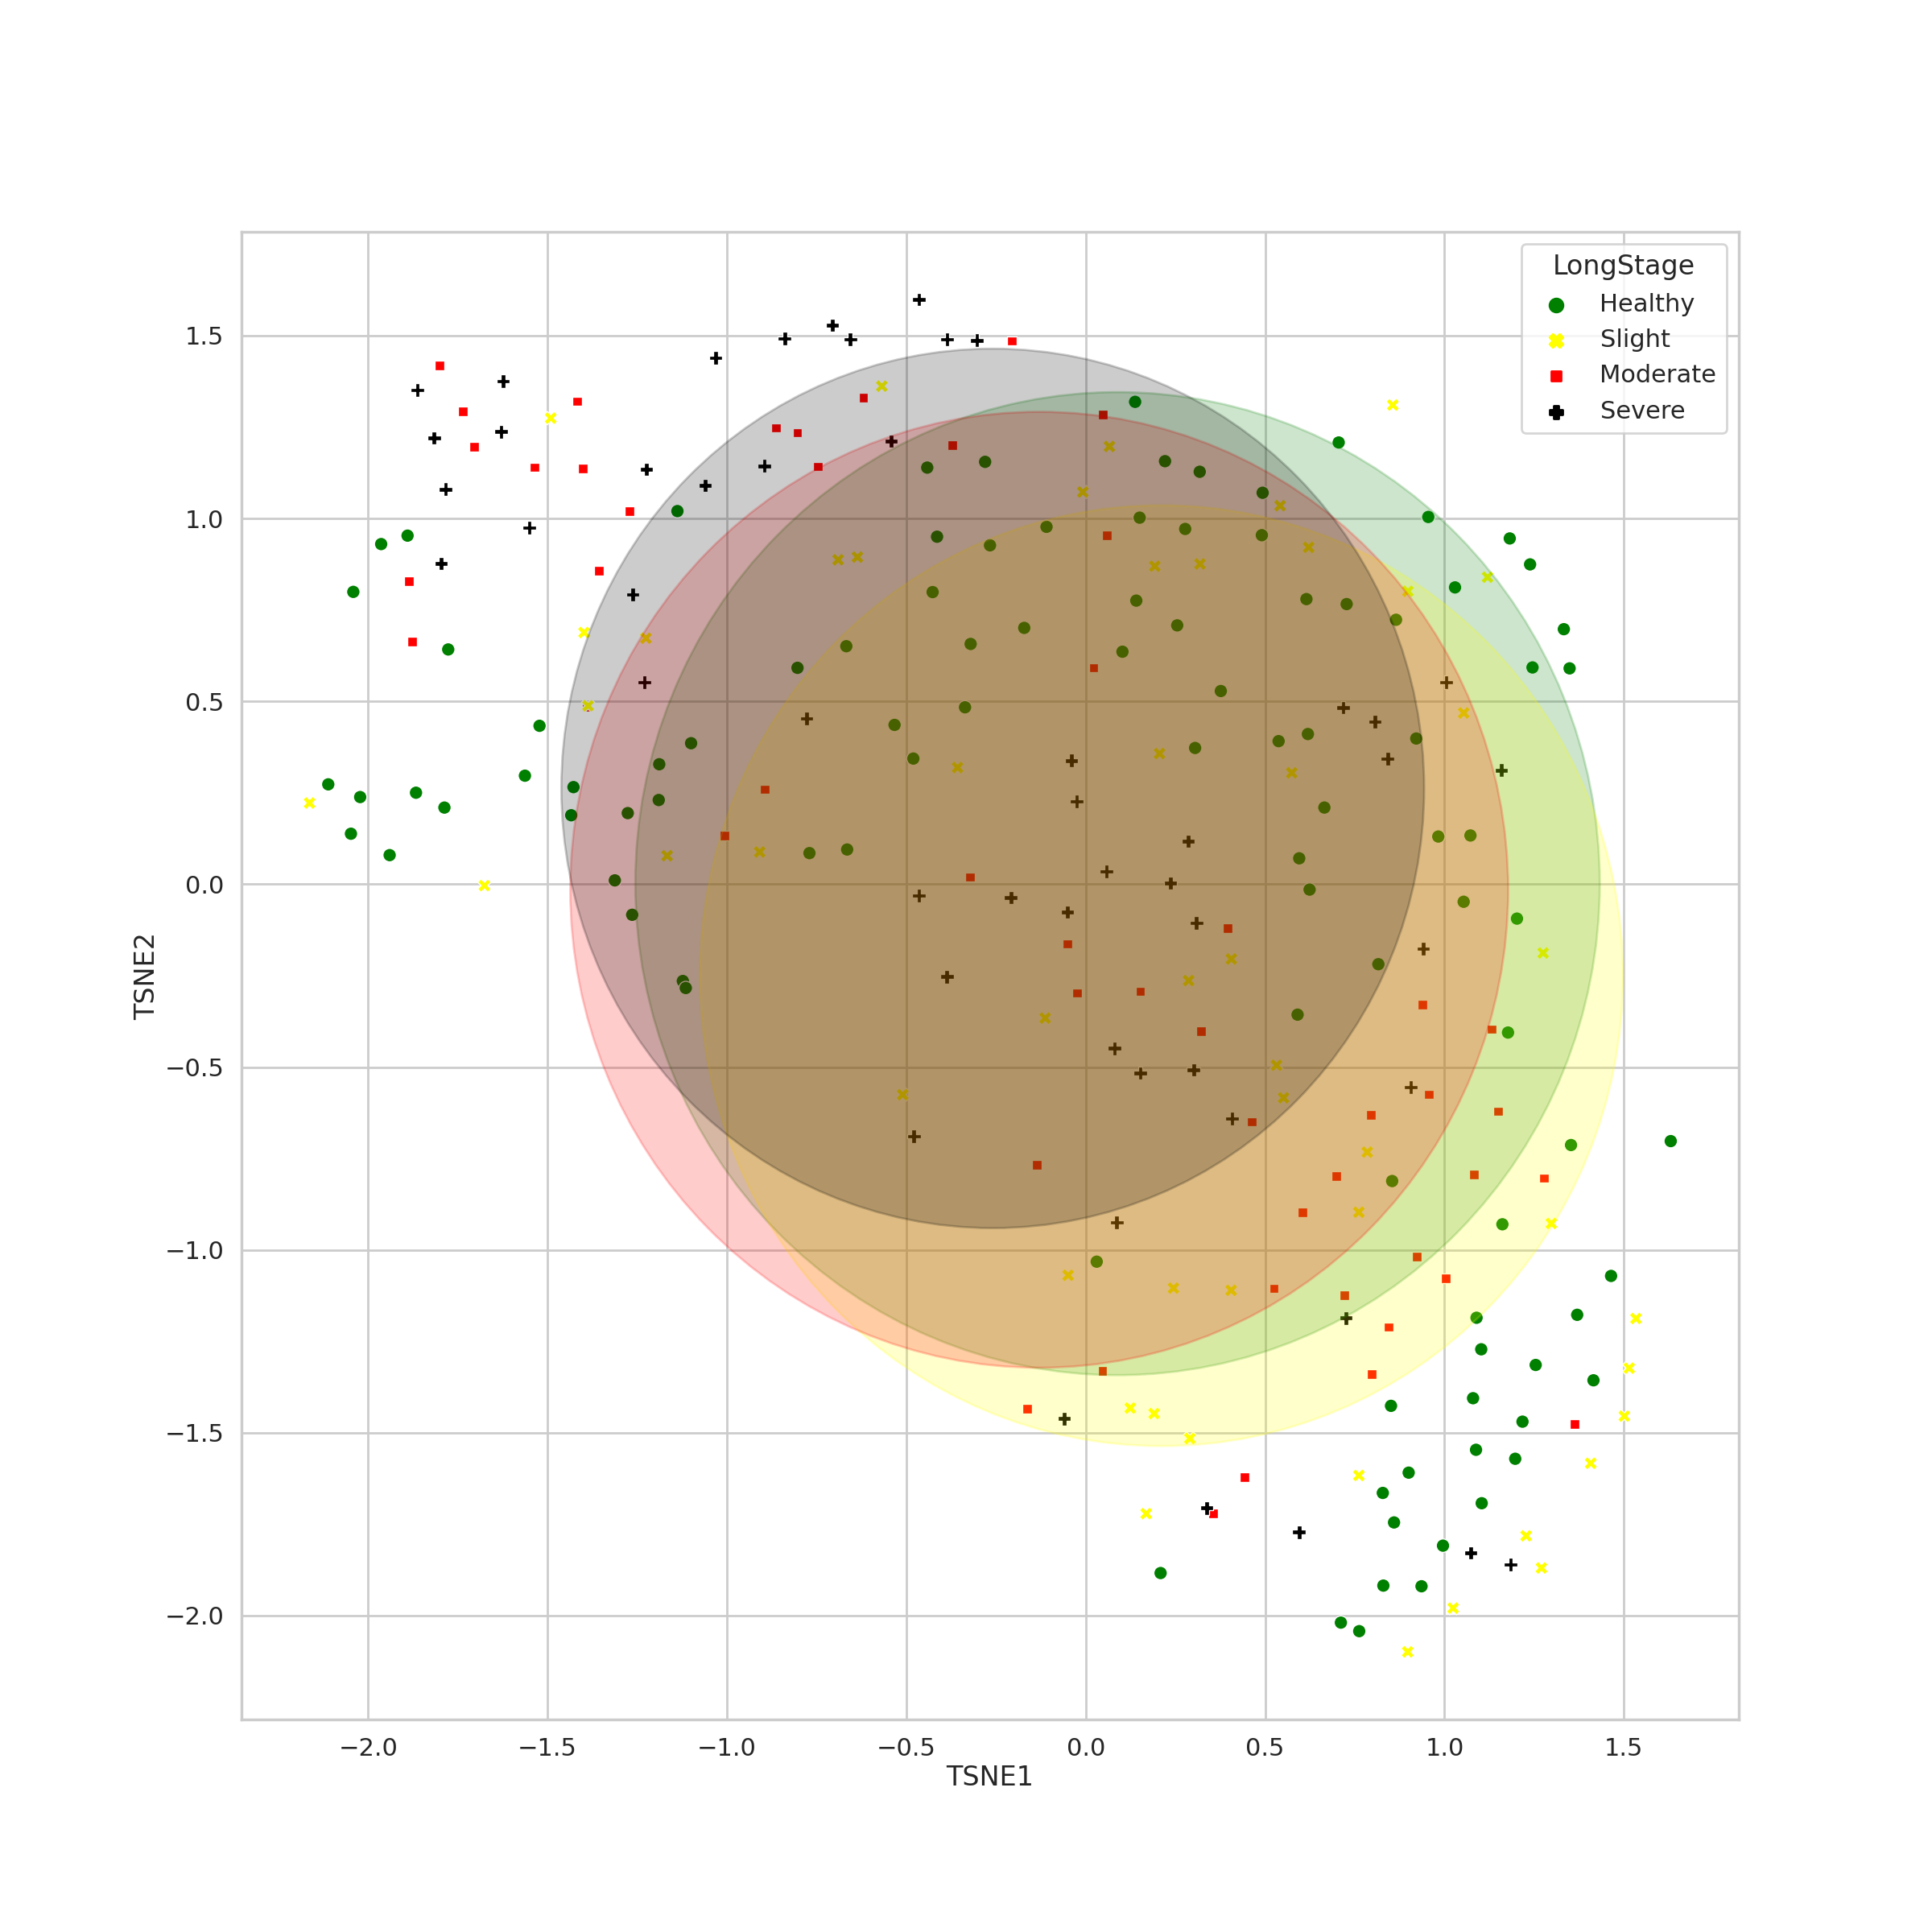
\includegraphics[width=0.6 \linewidth]{figures/BetaDiversity/Deblur.bray_curtis.png}
                \caption{t-SNE Plot from Bray-Curtis Distance Index with Deblur}
                \label{fig:tsne-bray-deblur}
            \end{figure}

            \begin{figure}[p]
                \centering
                $\begin{array}{cc}
                    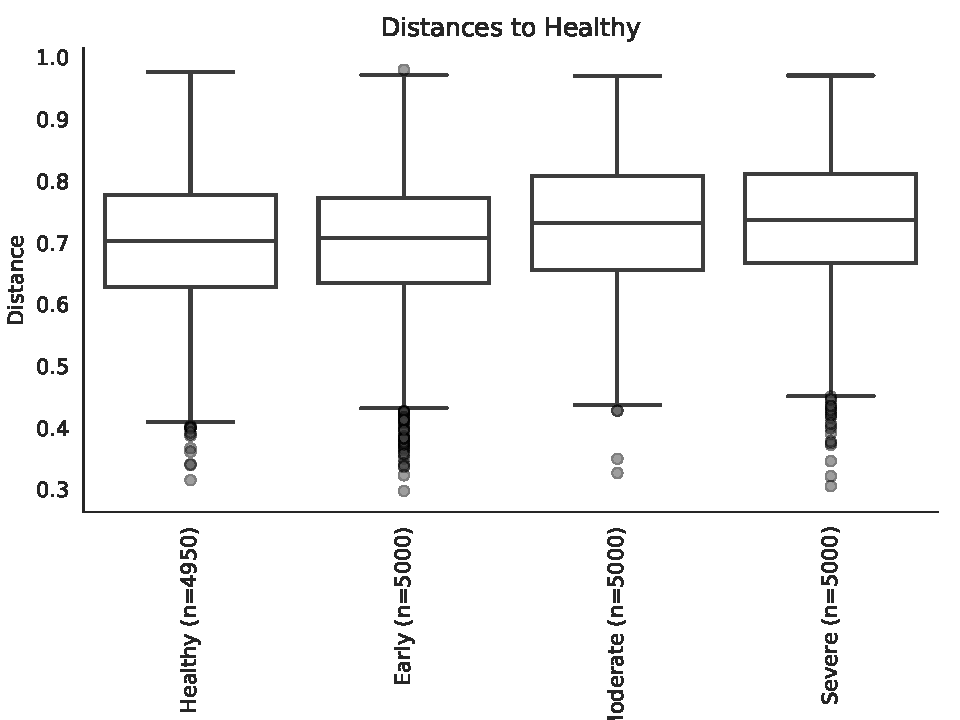
\includegraphics[width=0.4 \linewidth]{figures/BetaDiversity/Deblur/Bray/Healthy.pdf}
                    &
                    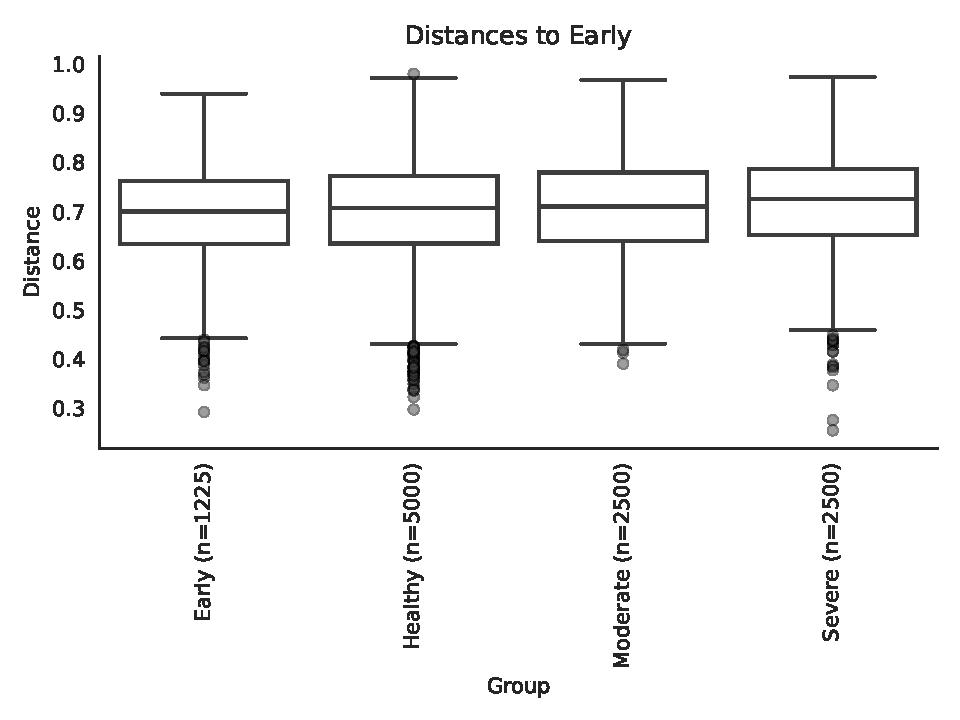
\includegraphics[width=0.4 \linewidth]{figures/BetaDiversity/Deblur/Bray/Early.pdf}
                    \\
                    \mbox{(a) Healthy} & \mbox{(b) Early} \\

                    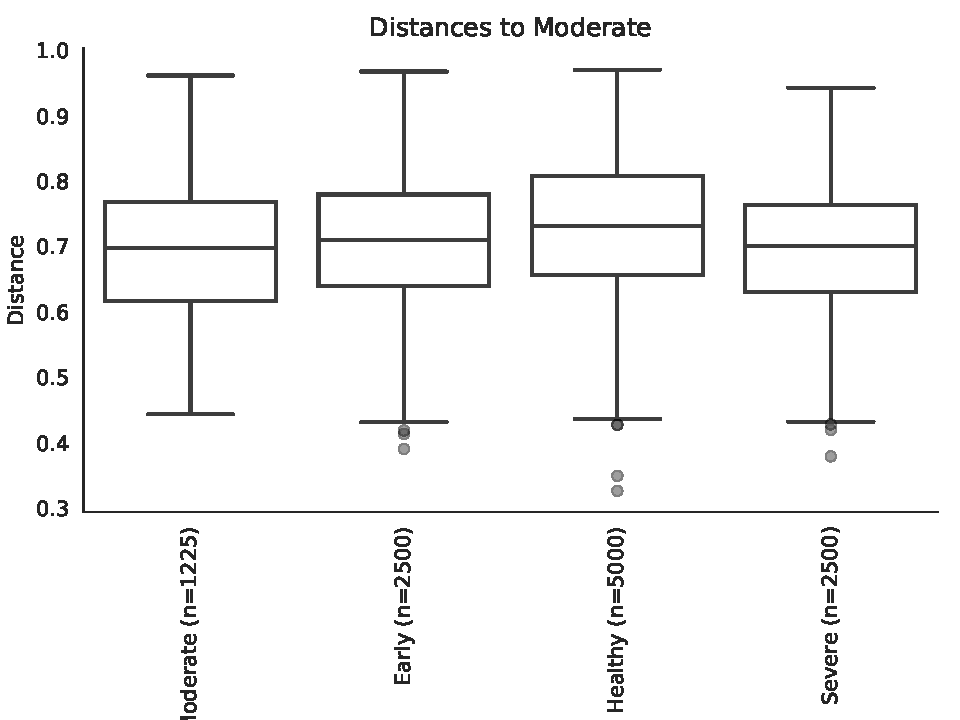
\includegraphics[width=0.4 \linewidth]{figures/BetaDiversity/Deblur/Bray/Moderate.pdf}
                    &
                    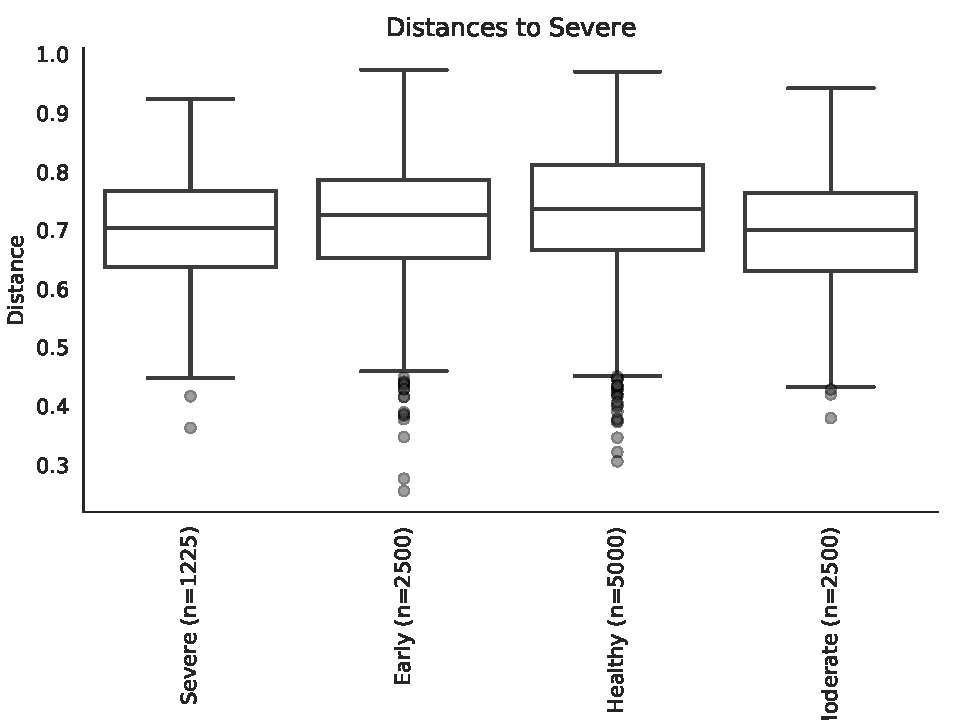
\includegraphics[width=0.4 \linewidth]{figures/BetaDiversity/Deblur/Bray/Severe.pdf}
                    \\
                    \mbox{(c) Moderate} & \mbox{(d) Severe} \\
                \end{array}$
                \caption{Bray-Curtis Distance Index with Deblur}
                \label{fig:bray-deblur}
            \end{figure}

            \begin{figure}[p]
                \centering
                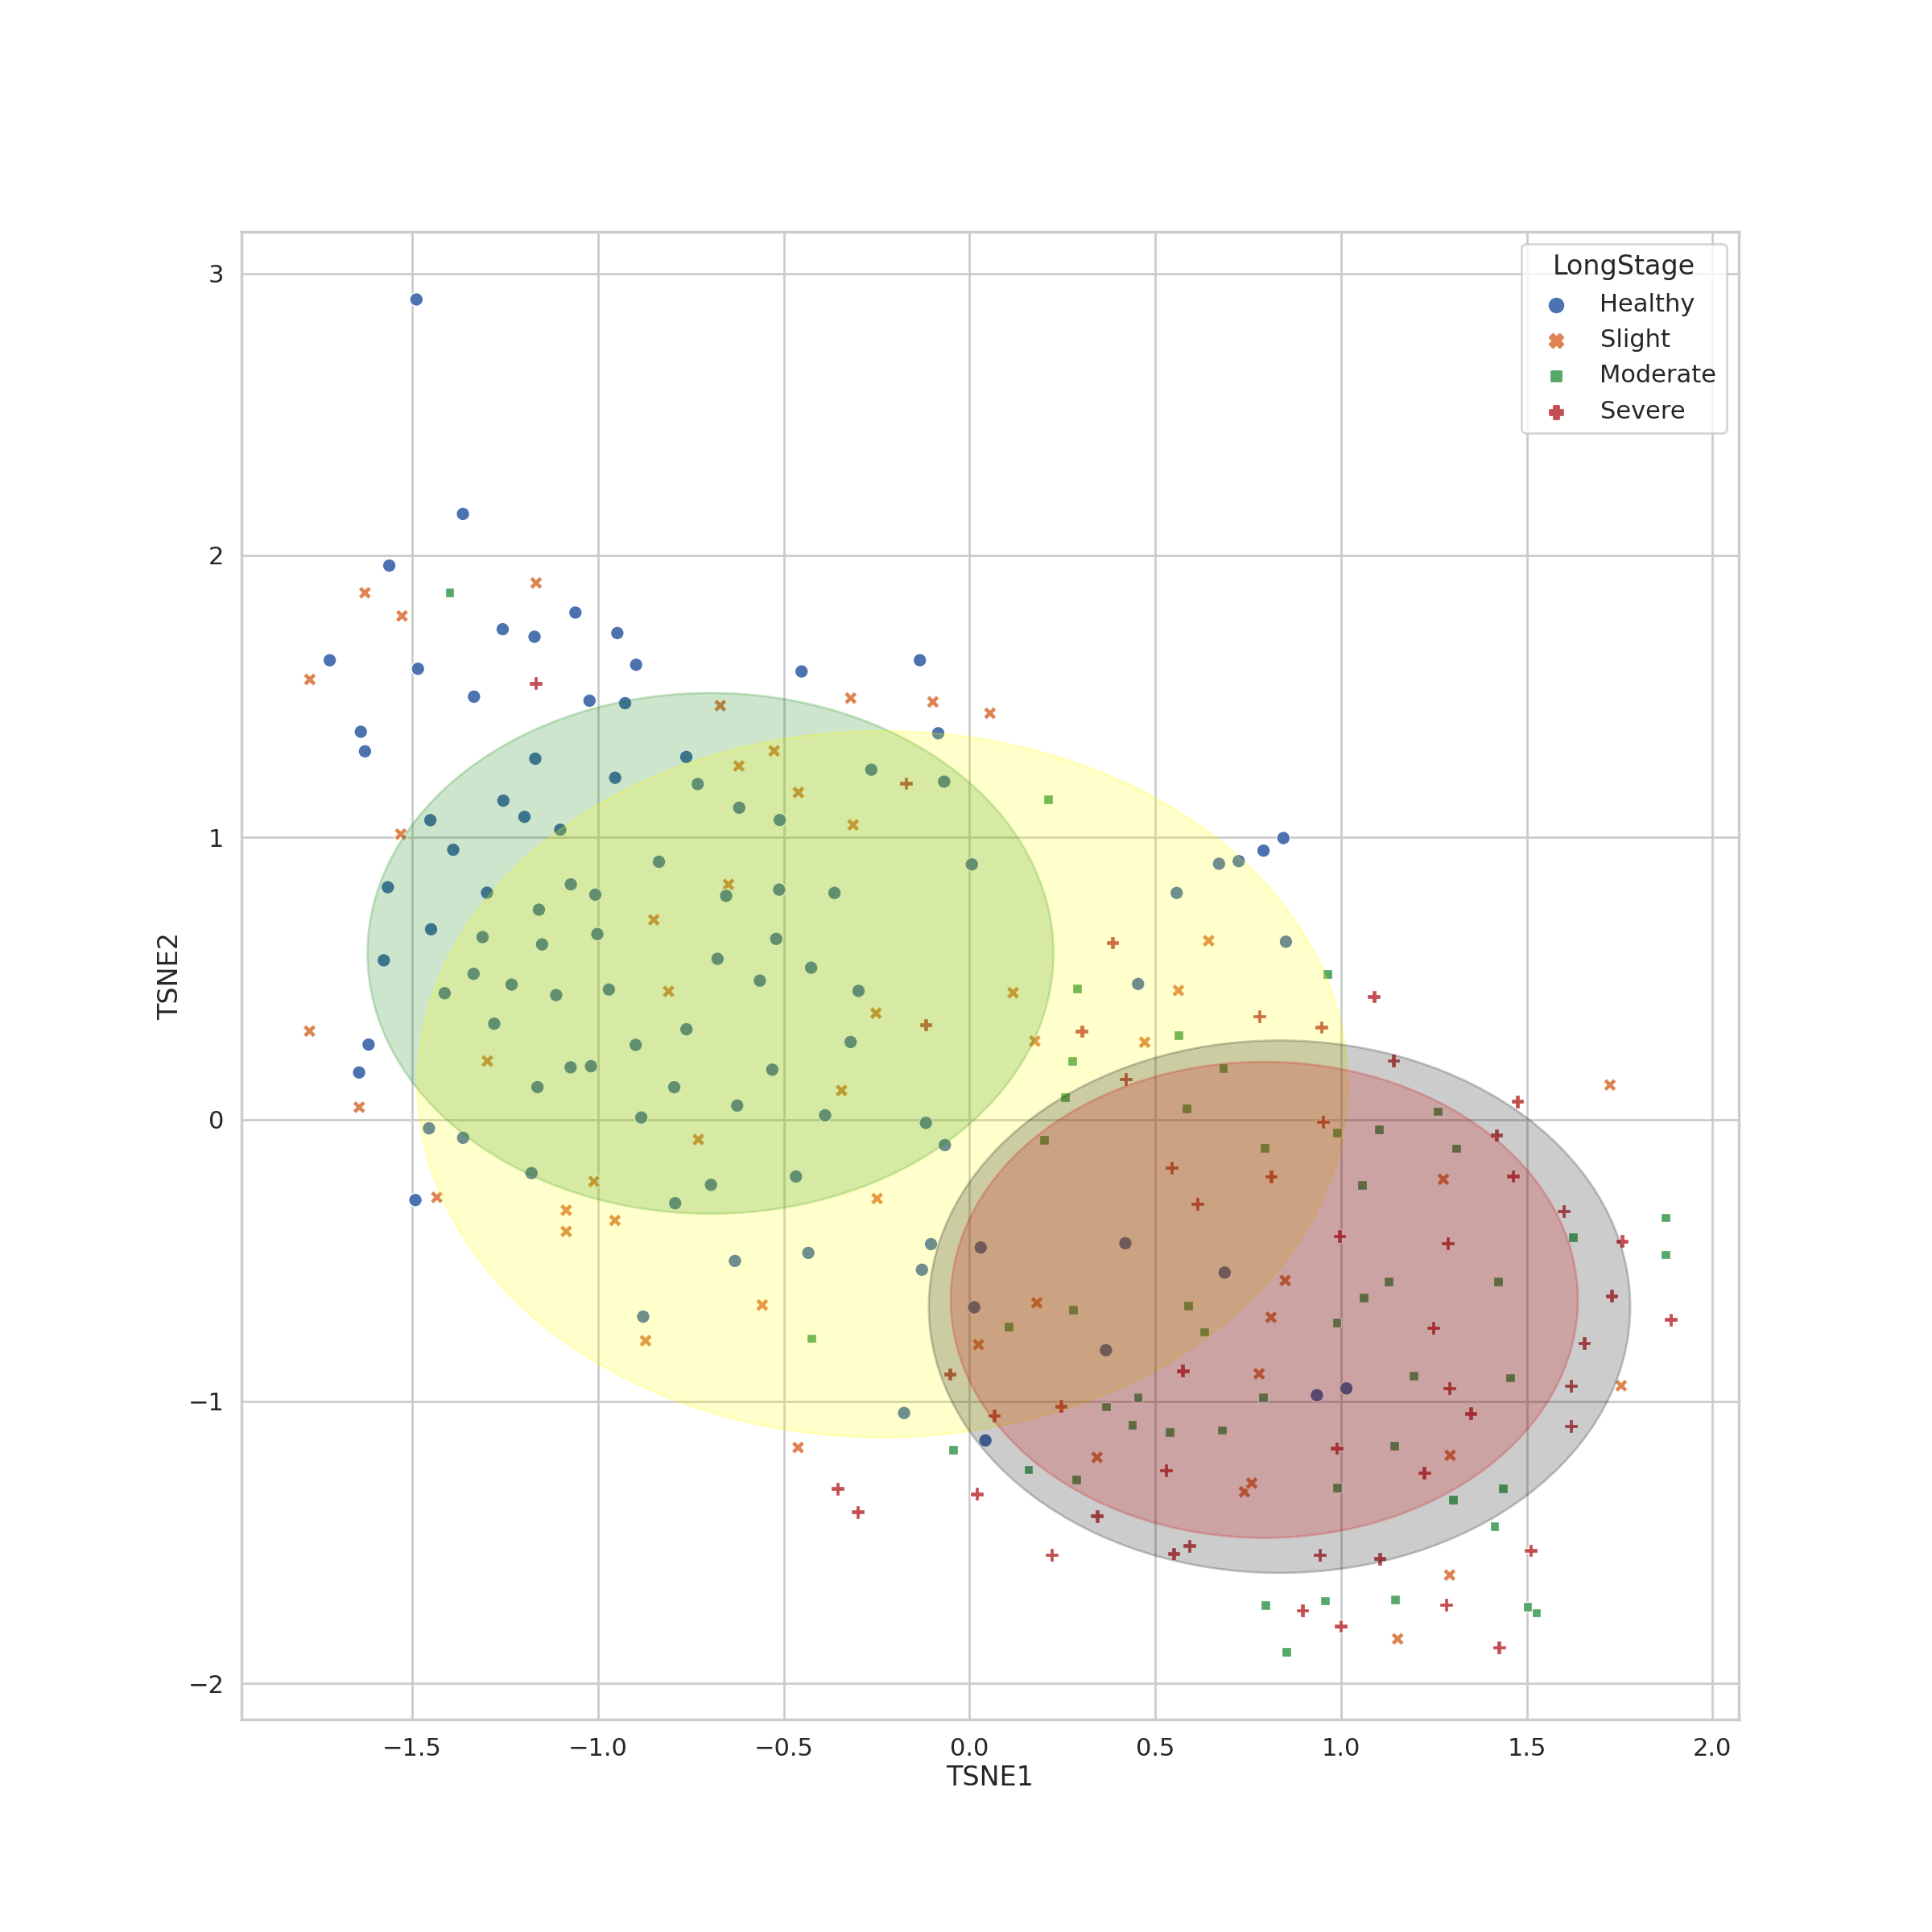
\includegraphics[width=0.6 \linewidth]{figures/BetaDiversity/Deblur.jaccard.png}
                \caption{t-SNE Plot from Jaccard Distance Index with Deblur}
                \label{fig:tsne-jaccard-deblur}
            \end{figure}

            \begin{figure}[p]
                \centering
                $\begin{array}{cc}
                    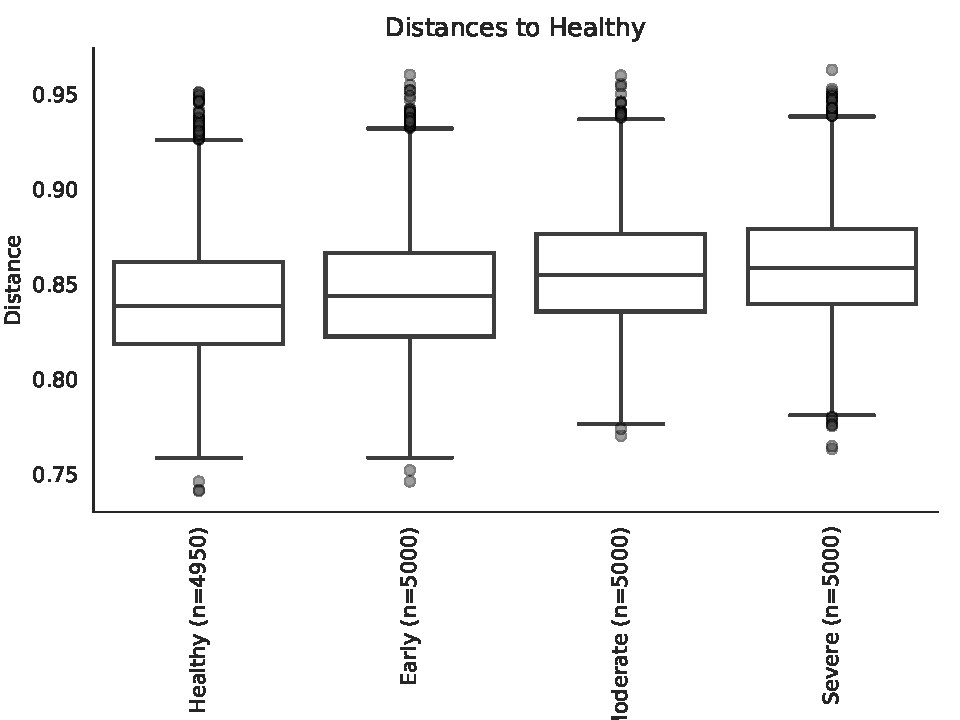
\includegraphics[width=0.4 \linewidth]{figures/BetaDiversity/Deblur/Jaccard/Healthy.pdf}
                    &
                    \includegraphics[width=0.4 \linewidth]{figures/BetaDiversity/Deblur/Jaccard/Early.pdf}
                    \\
                    \mbox{(a) Healthy} & \mbox{(b) Early} \\

                    \includegraphics[width=0.4 \linewidth]{figures/BetaDiversity/Deblur/Jaccard/Moderate.pdf}
                    &
                    \includegraphics[width=0.4 \linewidth]{figures/BetaDiversity/Deblur/Jaccard/Severe.pdf}
                    \\
                    \mbox{(c) Moderate} & \mbox{(d) Severe} \\
                \end{array}$
                \caption{Jaccard Distance Index with Deblur}
                \label{fig:jaccard-deblur}
            \end{figure}

            \begin{figure}[p]
                \centering
                \includegraphics[width=0.6 \linewidth]{figures/BetaDiversity/Deblur.unweighted_unifrac.png}
                \caption{t-SNE Plot from Unweighted UniFrac Distance Index with Deblur}
                \label{fig:tsne-unweighted-deblur}
            \end{figure}

            \begin{figure}[p]
                \centering
                $\begin{array}{cc}
                    \includegraphics[width=0.4 \linewidth]{figures/BetaDiversity/Deblur/UnweightedUnifrac/Healthy.pdf}
                    &
                    \includegraphics[width=0.4 \linewidth]{figures/BetaDiversity/Deblur/UnweightedUnifrac/Early.pdf}
                    \\
                    \mbox{(a) Healthy} & \mbox{(b) Early} \\

                    \includegraphics[width=0.4 \linewidth]{figures/BetaDiversity/Deblur/UnweightedUnifrac/Moderate.pdf}
                    &
                    \includegraphics[width=0.4 \linewidth]{figures/BetaDiversity/Deblur/UnweightedUnifrac/Severe.pdf}
                    \\
                    \mbox{(c) Moderate} & \mbox{(d) Severe} \\
                \end{array}$
                \caption{Unweighted UniFrac Distance Index with Deblur}
                \label{fig:unweighted-deblur}
            \end{figure}

            \begin{figure}[p]
                \centering
                \includegraphics[width=0.6 \linewidth]{figures/BetaDiversity/Deblur.weighted_unifrac.png}
                \caption{t-SNE Plot from Weighted UniFrac Distance Index with Deblur}
                \label{fig:tsne-weighted-deblur}
            \end{figure}

            \begin{figure}[p]
                \centering
                $\begin{array}{cc}
                    \includegraphics[width=0.4 \linewidth]{figures/BetaDiversity/Deblur/WeightedUnifrac/Healthy.pdf}
                    &
                    \includegraphics[width=0.4 \linewidth]{figures/BetaDiversity/Deblur/WeightedUnifrac/Early.pdf}
                    \\
                    \mbox{(a) Healthy} & \mbox{(b) Early} \\

                    \includegraphics[width=0.4 \linewidth]{figures/BetaDiversity/Deblur/WeightedUnifrac/Moderate.pdf}
                    &
                    \includegraphics[width=0.4 \linewidth]{figures/BetaDiversity/Deblur/WeightedUnifrac/Severe.pdf}
                    \\
                    \mbox{(c) Moderate} & \mbox{(d) Severe} \\
                \end{array}$
                \caption{Weighted UniFrac Distance Index with Deblur}
                \label{fig:weighted-deblur}
            \end{figure}

        \subsection{ANCOM}
            Statistically significant different taxa and volcano plots by ANCOM were derived: DADA2 and GG (Table \ref{tb:ANCOM-dada2-gg} and Figure \ref{fig:volcano-dada2-gg}), DADA2 and SILVA (Table \ref{tb:ANCOM-dada2-silva} and Figure \ref{fig:volcano-dada2-silva}), DADA2 and HOMD (Table \ref{tb:ANCOM-dada2-homd} and Figure \ref{fig:volcano-dada2-homd}), Deblur and GG (Table \ref{tb:ANCOM-deblur-gg} and Figure \ref{fig:volcano-deblur-gg}), Deblur and SILVA (Table \ref{tb:ANCOM-deblur-silva} and Figure \ref{fig:volcano-deblur-silva}) and Deblur and HOMD (Table \ref{tb:ANCOM-deblur-homd} and Figure \ref{fig:volcano-deblur-homd}).

            \begin{table}[p]
                \centering
                \caption{ANCOM Significant Taxa with DADA2 and GG}
                \label{tb:ANCOM-dada2-gg}

                \csvreader[tabular=p{10cm}cc, no head, column count=3, table head=\hline, late after first line=\\\hline, table foot=\hline, respect underscore]{csv/ANCOM/DADA2.gg.csv}{}{\csvlinetotablerow}
            \end{table}

            \begin{figure}[p]
                \centering
                \includegraphics[width=0.8 \linewidth]{figures/ANCOM/DADA2.gg.png}
                \caption{ANCOM Volcano Plot with DADA2 and GG}
                \label{fig:volcano-dada2-gg}
            \end{figure}

            \begin{table}[p]
                \centering
                \caption{ANCOM Significant Taxa with DADA2 and SILVA}
                \label{tb:ANCOM-dada2-silva}

                \csvreader[tabular=p{10cm}cc, no head, column count=3, table head=\hline, late after first line=\\\hline, table foot=\hline, respect underscore]{csv/ANCOM/DADA2.silva.csv}{}{\csvlinetotablerow}
            \end{table}

            \begin{figure}[p]
                \centering
                \includegraphics[width=0.8 \linewidth]{figures/ANCOM/DADA2.silva.png}
                \caption{ANCOM Volcano Plot with DADA2 and HOMD}
                \label{fig:volcano-dada2-silva}
            \end{figure}

            \begin{table}[p]
                \centering
                \caption{ANCOM Significant Taxa with DADA2 and HOMD}
                \label{tb:ANCOM-dada2-homd}

                \csvreader[tabular=p{10cm}cc, no head, column count=3, table head=\hline, late after first line=\\\hline, table foot=\hline, respect underscore]{csv/ANCOM/DADA2.homd.csv}{}{\csvlinetotablerow}
            \end{table}

            \begin{figure}[p]
                \centering
                \includegraphics[width=0.8 \linewidth]{figures/ANCOM/DADA2.homd.png}
                \caption{ANCOM Volcano Plot with DADA2 and SILVA}
                \label{fig:volcano-dada2-homd}
            \end{figure}

            \begin{table}[p]
                \centering
                \caption{ANCOM Significant Taxa with Deblur and GG}
                \label{tb:ANCOM-deblur-gg}

                \csvreader[tabular=p{10cm}cc, no head, column count=3, table head=\hline, late after first line=\\\hline, table foot=\hline, respect underscore]{csv/ANCOM/Deblur.gg.csv}{}{\csvlinetotablerow}
            \end{table}

            \begin{figure}[p]
                \centering
                \includegraphics[width=0.8 \linewidth]{figures/ANCOM/Deblur.gg.png}
                \caption{ANCOM Volcano Plot with Deblur and GG}
                \label{fig:volcano-deblur-gg}
            \end{figure}

            \begin{table}[p]
                \centering
                \caption{ANCOM Significant Taxa with Deblur and SILVA}
                \label{tb:ANCOM-deblur-silva}

                \csvreader[tabular=p{10cm}cc, no head, column count=3, table head=\hline, late after first line=\\\hline, table foot=\hline, respect underscore]{csv/ANCOM/DADA2.silva.csv}{}{\csvlinetotablerow}
            \end{table}

            \begin{figure}[p]
                \centering
                \includegraphics[width=0.8 \linewidth]{figures/ANCOM/Deblur.silva.png}
                \caption{ANCOM Volcano Plot with Deblur and SILVA}
                \label{fig:volcano-deblur-silva}
            \end{figure}

            \begin{table}[p]
                \centering
                \caption{ANCOM Significant Taxa with Deblur and HOMD}
                \label{tb:ANCOM-deblur-homd}

                \csvreader[tabular=p{10cm}cc, no head, column count=3, table head=\hline, late after first line=\\\hline, table foot=\hline, respect underscore]{csv/ANCOM/Deblur.homd.csv}{}{\csvlinetotablerow}
            \end{table}

            \begin{figure}[p]
                \centering
                \includegraphics[width=0.8 \linewidth]{figures/ANCOM/Deblur.homd.png}
                \caption{ANCOM Volcano Plot with Deblur and HOMD}
                \label{fig:volcano-deblur-homd}
            \end{figure}

        \subsection{t-SNE Plot with Whole Microbiome}
            As mentioned herein-before, t-SNE is a technique which reduce multi-dimensional data into two-dimension. Whole microbiome data are multi-dimensional data, which have \textit{circa} 600 columns, so the data should be reduced their dimension for readability. Hence, by the grace of t-SNE, the microbiome data have been deflated their dimension: 328 taxa from DADA2 and GG (Figure \ref{fig:tsne-whole-dada2-gg}), 633 taxa from DADA2 and SILVA (Figure \ref{fig:tsne-whole-dada2-silva}), 425 taxa from DADA2 and HOMD (Figure \ref{fig:tsne-whole-dada2-homd}), 232 taxa from Deblur and GG (Figure \ref{fig:tsne-whole-deblur-gg}), 414 taxa from Deblur and SILVA (Figure \ref{fig:tsne-whole-deblur-silva}) and 235 taxa from Deblur and HOMD (Figure \ref{fig:tsne-whole-deblur-homd}).

            \begin{figure}[p]
                \centering
                \includegraphics[width=0.6 \linewidth]{figures/tSNE/Whole/whole.DADA2.gg.png}
                \caption{t-SNE Plot with Whole Microbiome from DADA2 and GG (328 taxa)}
                \label{fig:tsne-whole-dada2-gg}
            \end{figure}

            \begin{figure}[p]
                \centering
                \includegraphics[width=0.6 \linewidth]{figures/tSNE/Whole/whole.DADA2.silva.png}
                \caption{t-SNE Plot with Whole Microbiome from DADA2 and SILVA (633 taxa)}
                \label{fig:tsne-whole-dada2-silva}
            \end{figure}

            \begin{figure}[p]
                \centering
                \includegraphics[width=0.6 \linewidth]{figures/tSNE/Whole/whole.DADA2.homd.png}
                \caption{t-SNE Plot with Whole Microbiome from DADA2 and HOMD (425 taxa)}
                \label{fig:tsne-whole-dada2-homd}
            \end{figure}

            \begin{figure}[p]
                \centering
                \includegraphics[width=0.6 \linewidth]{figures/tSNE/Whole/whole.Deblur.gg.png}
                \caption{t-SNE Plot with Whole Microbiome from Deblur and GG (232 taxa)}
                \label{fig:tsne-whole-deblur-gg}
            \end{figure}

            \begin{figure}[p]
                \centering
                \includegraphics[width=0.6 \linewidth]{figures/tSNE/Whole/whole.Deblur.silva.png}
                \caption{t-SNE Plot with Whole Microbiome from Deblur and SILVA (414 taxa)}
                \label{fig:tsne-whole-deblur-silva}
            \end{figure}

            \begin{figure}[p]
                \centering
                \includegraphics[width=0.6 \linewidth]{figures/tSNE/Whole/whole.Deblur.homd.png}
                \caption{t-SNE Plot with Whole Microbiome from Deblur and HOMD (235 taxa)}
                \label{fig:tsne-whole-deblur-homd}
            \end{figure}

        \subsection{t-SNE Plot with ANCOM Selected Microbiome Data}
            As whole microbiome data, ANCOM selected microbiome data are also multi-dimensional data, even though their columns are selected by ANCOM. Hence, with t-SNE, ANCOM selected microbiome data have also been deflated their dimension: 15 taxa (as Table \ref{tb:ANCOM-dada2-gg}) from DADA2 and GG (Figure \ref{fig:tsne-ANCOM-dada2-gg}), 23 taxa (as Table \ref{tb:ANCOM-dada2-silva}) from DADA2 and SILVA (Figure \ref{fig:tsne-ANCOM-dada2-silva}), 20 taxa (as Table \ref{tb:ANCOM-dada2-homd}) from DADA2 and HOMD (Figure \ref{fig:tsne-ANCOM-dada2-homd}), 27 taxa (as Table \ref{tb:ANCOM-deblur-gg}) from Deblur and GG (Figure \ref{fig:tsne-whole-deblur-gg}), 20 taxa (as Table \ref{tb:ANCOM-deblur-silva}) from Deblur and SILVA (Figure \ref{fig:tsne-ANCOM-deblur-silva}) and 28 taxa (as Table \ref{tb:ANCOM-deblur-homd}) from Deblur and HOMD (Figure \ref{fig:tsne-ANCOM-deblur-homd}).

            \begin{figure}[p]
                \centering
                \includegraphics[width=0.6 \linewidth]{figures/tSNE/ANCOM/ANCOM.DADA2.gg.png}
                \caption{t-SNE Plot with ANCOM Selected Microbiome Data from DADA2 and GG (15 taxa)}
                \label{fig:tsne-ANCOM-dada2-gg}
            \end{figure}

            \begin{figure}[p]
                \centering
                \includegraphics[width=0.6 \linewidth]{figures/tSNE/ANCOM/ANCOM.DADA2.silva.png}
                \caption{t-SNE Plot with ANCOM Selected Microbiome Data from DADA2 and SILVA (23 taxa)}
                \label{fig:tsne-ANCOM-dada2-silva}
            \end{figure}

            \begin{figure}[p]
                \centering
                \includegraphics[width=0.6 \linewidth]{figures/tSNE/ANCOM/ANCOM.DADA2.homd.png}
                \caption{t-SNE Plot with ANCOM Selected Microbiome Data from DADA2 and HOMD (20 taxa)}
                \label{fig:tsne-ANCOM-dada2-homd}
            \end{figure}

            \begin{figure}[p]
                \centering
                \includegraphics[width=0.6 \linewidth]{figures/tSNE/ANCOM/ANCOM.Deblur.gg.png}
                \caption{t-SNE Plot with ANCOM Selected Microbiome Data from Deblur and GG (27 taxa)}
                \label{fig:tsne-ANCOM-deblur-gg}
            \end{figure}

            \begin{figure}[p]
                \centering
                \includegraphics[width=0.6 \linewidth]{figures/tSNE/ANCOM/ANCOM.Deblur.silva.png}
                \caption{t-SNE Plot with ANCOM Selected Microbiome Data from Deblur and SILVA (20 taxa)}
                \label{fig:tsne-ANCOM-deblur-silva}
            \end{figure}

            \begin{figure}[p]
                \centering
                \includegraphics[width=0.6 \linewidth]{figures/tSNE/ANCOM/ANCOM.Deblur.homd.png}
                \caption{t-SNE Plot with ANCOM Selected Microbiome Data from Deblur and HOMD (28 taxa)}
                \label{fig:tsne-ANCOM-deblur-homd}
            \end{figure}

        \subsection{Random Forest Classifier with Every Class}
            As figure \ref{fig:denosing-workflow} and figure \ref{fig:taxonomy-workflow}, there are six combinations. Thus, classification algorithm is carried out on these six combinations (Figure \ref{fig:RF-whole-workflow}). Among these six combinations, Deblur and HOMD pair gives the best result in terms of balanced accuracy. Features which are ordered by importance are table \ref{tb:RF-every-Deblur-homd}. Also, five metrics by feature count are shown as figure \ref{fig:RF-every-metrics-Deblur-homd}; then, the highest value of balanced accuracy is 0.778 with using 13 taxa. Moreover, violin plots from two most important taxa, \textit{Porphyromonas gingivalis} and {(b) \textit{Actinomyces}, are in figure \ref{fig:RF-every-important-Deblur-homd}.

            \begin{table}[p]
                \centering
                \caption{Taxa with Deblur and HOMD Ordered by Random Forest}
                \label{tb:RF-every-Deblur-homd}

                \csvreader[tabular=cp{10cm}l, no head, column count=3, table head=\hline, late after first line=\\\hline, table foot=\hline]{csv/RandomForest/whole-Deblur-homd.txt}{}{\csvlinetotablerow}
            \end{table}

            \begin{figure}[p]
                \centering
                \includegraphics[width=0.7 \linewidth]{figures/RandomForest/ANCOM.Deblur.homd/metrics.png}
                \caption{Metrics by Feature Count with Deblur and HOMD}
                \label{fig:RF-every-metrics-Deblur-homd}
            \end{figure}

            \begin{figure}[p]
                \centering
                $\begin{array}{cc}
                    \includegraphics[width=0.4 \linewidth]{figures/RandomForest/ANCOM.Deblur.homd/Feature_0.png}
                    &
                    \includegraphics[width=0.4 \linewidth]{figures/RandomForest/ANCOM.Deblur.homd/Feature_1.png}
                    \\
                    \mbox{(a) \textit{Porphyromonas gingivalis}} & \mbox{(b) \textit{Actinomyces}} \\
                \end{array}$
                \caption{Most and Second Most Important Features with Deblur and HOMD}
                \label{fig:RF-every-important-Deblur-homd}
            \end{figure}

        \subsection{Random Forest Classifier with Merging (Healthy+Early) Classes}
            As figures \ref{fig:denosing-workflow} and \ref{fig:taxonomy-workflow}, there are six combinations. However, there is no significant difference between Healthy and Early classes. Thus, classification algorithm is carried out on these six combinations with merging Healthy and Early classes. Among these six combinations, DADA2 and HOMD pair gives the best result in terms of balanced accuracy.

            \begin{table}[p]
                \centering
                \caption{Taxa with DADA2 and HOMD Ordered by Random Forest for Merging (Healthy+Early) Classes}
                \label{tb:RF-HE-DADA2-homd}

                \csvreader[tabular=cp{10cm}l, no head, column count=3, table head=\hline, late after first line=\\\hline, table foot=\hline]{csv/RandomForest/one-DADA2-homd.txt}{}{\csvlinetotablerow}
            \end{table}

            \begin{figure}[p]
                \centering
                \includegraphics[width=0.7 \linewidth]{figures/RandomForest/one.DADA2.homd/metrics.png}
                \caption{Metrics by Feature Count with DADA2 and HOMD for Merging (Healthy+Early) Classes}
                \label{fig:RF-HE-metrics-DADA2-homd}
            \end{figure}

            \begin{figure}[p]
                \centering
                $\begin{array}{cc}
                    \includegraphics[width=0.4 \linewidth]{figures/RandomForest/one.DADA2.homd/Feature_0.png}
                    &
                    \includegraphics[width=0.4 \linewidth]{figures/RandomForest/one.DADA2.homd/Feature_1.png}
                    \\
                    \mbox{(a) \textit{Porphyromonas gingivalis}} & \mbox{(b) \textit{Actinomyces}} \\
                \end{array}$
                \caption{Most and Second Most Important Features with DADA2 and HOMD for Merging (Healthy+Early) Classes}
                \label{fig:RF-HE-important-DADA2-homd}
            \end{figure}

        \subsection{Random Forest Classifier with Merging (Moderate+Severe) Classes}

            \begin{table}[p]
                \centering
                \caption{Taxa with Deblur and HOMD Ordered by Random Forest for Merging (Moderate+Severe) Classes}
                \label{tb:RF-MS-Deblur-homd}

                \csvreader[tabular=cp{10cm}l, no head, column count=3, table head=\hline, late after first line=\\\hline, table foot=\hline]{csv/RandomForest/two-Deblur-homd.txt}{}{\csvlinetotablerow}
            \end{table}

            \begin{figure}[p]
                \centering
                \includegraphics[width=0.7 \linewidth]{figures/RandomForest/two.Deblur.homd/metrics.png}
                \caption{Metrics by Feature Count with Deblur and HOMD for Merging (Moderate+Severe) Classes}
                \label{fig:RF-MS-metrics-Deblur-homd}
            \end{figure}

            \begin{figure}[p]
                \centering
                $\begin{array}{cc}
                    \includegraphics[width=0.4 \linewidth]{figures/RandomForest/two.Deblur.homd/Feature_0.png}
                    &
                    \includegraphics[width=0.4 \linewidth]{figures/RandomForest/two.Deblur.homd/Feature_1.png}
                    \\
                    \mbox{(a) \textit{Porphyromonas gingivalis}} & \mbox{(b) \textit{Actinomyces}} \\
                \end{array}$
                \caption{Most and Second Most Important Features with Deblur and HOMD for Merging (Moderate+Severe) Classes}
                \label{fig:RF-MS-important-Deblur-homd}
            \end{figure}

        \subsection{Random Forest Classifier with Merging (Healthy+Early) \& (Moderate+Severe) Classes}

            \begin{table}[p]
                \centering
                \caption{Taxa with DADA2 and SILVA Ordered by Random Forest for Merging (Healthy+Early) \& (Moderate+Severe) Classes}
                \label{tb:RF-HEMS-DADA2-silva}

                \csvreader[tabular=cp{10cm}l, no head, column count=3, table head=\hline, late after first line=\\\hline, table foot=\hline]{csv/RandomForest/onetwo-DADA2-silva.txt}{}{\csvlinetotablerow}
            \end{table}

            \begin{figure}[p]
                \centering
                \includegraphics[width=0.7 \linewidth]{figures/RandomForest/one-two.DADA2.silva/metrics.png}
                \caption{Metrics by Feature Count with DADA2 and SILVA for Merging (Healthy+Early) \& (Moderate+Severe) Classes}
                \label{fig:RF-HEMS-metrics-DADA2-silva}
            \end{figure}

            \begin{figure}[p]
                \centering
                $\begin{array}{cc}
                    \includegraphics[width=0.4 \linewidth]{figures/RandomForest/one-two.DADA2.silva/Feature_0.png}
                    &
                    \includegraphics[width=0.4 \linewidth]{figures/RandomForest/one-two.DADA2.silva/Feature_1.png}
                    \\
                    \mbox{(a) \textit{Porphyromonas gingivalis}} & \mbox{(b) \textit{Treponema denticola}} \\
                \end{array}$
                \caption{Most and Second Most Important Features with Deblur and HOMD for Merging (Healthy+Early) \& (Moderate+Severe) Classes}
                \label{fig:RF-HEMS-important-DADA2-silva}
            \end{figure}

        \subsection{Random Forest Classifier with Healthy Class and Early Class Only}

    \section{Discussion}
        \subsection{Alpha-diversity}
            Alpha-diversity indices among all groups from DADA2 are in table \ref{tb:alpha-all-dada2}. Shannon's diversity index in DADA2, though, has marginally significant p-value; the other indices have strongly significant p-values. Additionally, there are no statistically significant differences between (Healthy and Early) classes and (Moderate and Severe) classes with evenness index from DADA2 (Table \ref{tb:alpha-evenness-dada2} and Figure \ref{fig:evenness-dada2}). Also, there is no statistically significant difference between (Healthy and Early) classes with Faith's phylogenetic diversity index from DADA2 (Table \ref{tb:alpha-faith-dada2} and Figure \ref{fig:faith-dada2}). Moreover, there are no statistically significant differences between (Early and Moderate) classes, (Early and Severe) classes and (Moderate and Severe) classes with observed feature index from DADA2 (Table \ref{tb:alpha-observed-dada2} and Figure \ref{fig:observed-dada2}). Furthermore, there are no statistically significant differences between (Healthy and Moderate) classes, (Healthy and Severe) classes, (Early and Moderate) classes and (Moderate and Severe) classes from Shannon's diversity index from DADA2 (Table \ref{tb:alpha-shannon-dada2} and Figure \ref{fig:shannon-dada2}).

            Alpha-diversity indices among all groups from Deblur are in table \ref{tb:alpha-all-deblur}. Every index have strongly significant p-values. Additionally, there are no statistically significant differences between (Healthy and Early) classes, (Healthy and Moderate) classes, (Healthy and Severe) classes and (Moderate and Severe) classes with evenness index from Deblur (Table \ref{tb:alpha-evenness-deblur} and Figure \ref{fig:evenness-deblur}). Also, there are no statistically significant differences between (Healthy and Early) classes and (Moderate and Severe) classes with Faith's phylogenetic diversity index from Deblur (Table \ref{tb:alpha-faith-deblur} and Figure \ref{fig:faith-deblur}). Moreover, there are no statistically significant differences between (Healthy and Early) classes and (Moderate and Severe) classes with observed features index from Deblur (Table \ref{tb:alpha-observed-deblur} and Figure \ref{fig:observed-deblur}). Furthermore, there are no statistically significant differences between (Healthy and Early) classes and (Moderate and Severe) classes with Shannon's diversity index from Deblur (Table \ref{tb:alpha-shannon-deblur} and Figure \ref{fig:shannon-deblur}).

            Merging similar classes could elevate classification metrics; while merging must result mere primitive classification than without merging classes. Accordingly, deciding merged classes should be rigorous and resolutely reasoned. In result, many pairs of classes should be merged as value of alpha-diversity indices, for instance (Healthy and Early) classes, (Healthy and Severe) classes and (Moderate and Severe) classes. Despite alpha-diversity indices show no significant differences, some pairs of classes have to refuse to be merged in two major reasons. First, merging those classes is fallacious. For example, (Healthy and Severe) classes, without loss of generality. Healthy class and Severe class does not adjoin each other, in terms of clinical stage. Second, even those classes are adjacent each other, some pairs of classes have not enough results to merge. For instance, null hypothesis from (Early and Moderate) classes is only sustained by Shannon's diversity index (Table \ref{tb:alpha-shannon-dada2}), so merging Early class and Moderate class cannot be reasoned. Hence, two pairs of classes will be merged in classification: (Healthy and Early) classes and (Moderate and Severe) classes.

        \subsection{Beta-diversity}
            From data with DADA2, all beta-diversity distance index, includes Bray-Curtis distance index (Table \ref{tb:bray-dada2}, Figure \ref{fig:tsne-bray-dada2} and Figure \ref{fig:bray-dada2}), Jaccard distance index (Table \ref{tb:jaccard-dada2}, Figure \ref{fig:tsne-jaccard-dada2} and Figure \ref{fig:jaccard-dada2}), unweighted UniFrac distance index (Table \ref{tb:unweighted-dada2}, Figure \ref{fig:tsne-unweighted-dada2} and Figure \ref{fig:unweighted-dada2}) and weighted UniFrac distance index (Table \ref{tb:weighted-dada2}, Figure \ref{fig:tsne-weighted-dada2} and Figure \ref{fig:weighted-dada2}), show statistically significant differences in every pair of classes, except (Moderate and Severe) classes.

            Bray-Curtis distance index with Deblur has no statistically significant differences between (Healthy and Early) classes and (Moderate and Severe) classes (Table \ref{tb:bray-deblur}, Figure \ref{fig:tsne-bray-deblur} and Figure \ref{fig:bray-deblur}). Moreover, Jaccard distance index with Deblur has no statistically significant difference between (Moderate and Severe) classes (Table \ref{tb:jaccard-deblur}, Figure \ref{fig:tsne-jaccard-deblur} and Figure \ref{fig:jaccard-deblur}). Additionally, unweighted UniFrac distance index with Deblur has no statistically significant difference between (Moderate and Severe) classes (Table \ref{tb:unweighted-deblur}, Figure \ref{fig:tsne-unweighted-deblur} and Figure \ref{fig:unweighted-deblur}). Furthermore, weighted UniFrac distance index with Deblur has no statistically significant difference between (Healthy and Early) classes (Table \ref{fig:weighted-deblur}, Figure \ref{fig:tsne-weighted-deblur} and Figure \ref{fig:weighted-deblur}).

            As results of alpha-diversity indices, (Healthy and Early) classes and (Moderate and Severe) classes will be merged. Mercifully, alternative fact does totally not sustained by beta-divesity indices. Hence, (Healthy and Early) classes and (Moderate and Severe) classes, as mentioned herein-before, will be merged in classification.

        \subsection{t-SNE Plot}
            Overall distribution of taxa from each sample can be realized by t-SNE plot. If each class is evenly distributed on t-SNE plot, then the data might be difficult for classifying. In this manner, t-SNE plots with whole microbiome (Figure \ref{fig:tsne-whole-dada2-gg}, Figure \ref{fig:tsne-whole-dada2-silva}, Figure \ref{fig:tsne-whole-dada2-homd}, Figure \ref{fig:tsne-whole-deblur-gg}, Figure \ref{fig:tsne-whole-deblur-silva} and Figure \ref{fig:tsne-whole-deblur-homd}) are more evenly distributed, whereas t-SNE plots with ANCOM selected microbiome data (Figure \ref{fig:tsne-ANCOM-dada2-gg}, Figure \ref{fig:tsne-ANCOM-dada2-silva}, Figure \ref{fig:tsne-ANCOM-dada2-homd}, Figure \ref{fig:tsne-ANCOM-deblur-gg}, Figure \ref{fig:tsne-ANCOM-deblur-silva} and Figure \ref{fig:tsne-ANCOM-deblur-homd}) are biased by classes. \textit{Id est}, data with ANCOM selected microbiome could result better in classifying. Hence, ANCOM selected taxa will be used in classification.

        \subsection{Random Forest Classifier}

    \bibliographystyle{apacite}
    \bibliography{reference}
\end{document}